\documentclass[11pt]{book}
\usepackage{sty/BookIngSoftware}
\usepackage{sty/IS_Procesos}
\usepackage{apacite}
\usepackage[spanish]{babel}
\usepackage{multirow}
\usepackage{graphicx}
\usepackage{float}
\usepackage{longtable}
\usepackage[utf8]{inputenc}
\usepackage[usenames,dvipsnames]{color}

%\usepackage[round]{natbib}
%\usepackage[hyperfootnotes=false]{hyperref}
\definecolor{airforceblue}{rgb}{0.36, 0.54, 0.66}
\hypersetup{
 colorlinks,
 citecolor=airforceblue,
 %linkcolor=Red,
% urlcolor=Blue
}


%=======================================
% Head del Documento
\title{Herramienta para la vinculación laboral}

\subtitulo{Trabajo Terminal No. 2019-A001}



\author{Aburto Pérez Luis Mario}{Osorio Rodríguez Eslí Joana}{Zamora Galloso Fernando}


\organizacion{Escuela Superior de Cómputo, IPN}
\date{25 de octubre del 2019}

\begin{document}    


   
    \maketitle
   
    %%=======================================
    %% Indices
    \tableofcontents
    \listoftables
    \listoffigures
   
   %%%%%%%%%% DOCUMENTO 
   \chapter{Introducci\'on}


%%Colocar una descripción de lo que contiene el capítulo

En el presente trabajo se estudiará la problemática a la que se enfrentan muchos jóvenes al no poder encontrar una actividad productiva en la cual dediquen su tiempo, ya sea estudiar, trabajar o formarse de alguna otra forma.\\

Se identificará cuáles son los principales factores que influyen para que esta problemática se presente, así como una posible solución que combata algún factor de la problemática. %También se describirán algunos programas similares que fueron propuestos por el gobierno de México y Colombia para intentar detener el aumento de la población desocupada de su respectivo país. \\

%%Todo esto por medio de nuestro conocimiento en la rama de los sistemas computacionales para así tratar de dar una solución a esta problemática apoyándonos en las tecnologías a las que hoy en día casi cualquier persona tiene acceso (internet, Smartphone, etc.)

	   \section{Contexto de trabajo}

%%Se describe el área donde se esta trabajando y en qué 

%%Se propone tener una cobertura en la (zona metropolitana del país o CDMX), teniendo como población objetivo los jóvenes que no se encuentren trabajando o preparándose profesionalmente para incorporarse a la Población Económicamente Activa (PEA) al momento de registrarse en el sistema. 
Un joven debería ser parte de la fuerza laboral o bien, se debería preparar para entrar a ella. De no ser así —es decir, si ese joven no tiene un empleo, ya sea formal o informal, y tampoco se está preparando en alguna institución educativa para ingresar a la fuerza laboral—, se le clasifica como NINI. \\

Hoy día la tasa de ninis en México esta incrementado llegando a una cifra de 3.9 millones de personas según el \cite{INEGI} \cite{OECD2}, generando un costo anual de 194,000 millones de pesos.

 En Parametría se reportan los resultados de una encuesta de opinión en viviendas y donde 58 por ciento de los entrevistados opina que para los ninis resulta más atractivo entrar a las filas del narcotráfico que conseguir un trabajo o asistir a la escuela. \cite{Parametria} Además, en su análisis, Escobedo \cite{JEB} menciona que 80 por ciento de los ninis ha participado en actos de violencia, aunado a esto una encuesta realizada por la firma OCCMundial ocho de cada diez jóvenes mexicanos no se inscribieron a una universidad y 42 por ciento no lo hizo porque no pudo pagar una licenciatura de estudios presenciales por otra parte seis de cada diez jóvenes abandonaron sus estudios superiores por falta de dinero. \cite{OCC} \cite{Forbes_Universidad} \\
 \bigskip

	   %\addbibresource{referencias.bib}
\newpage
\section{Problemática}

Un joven debería ser parte de la Población Económicamente Activa (PEA), o bien, se debería preparar para entrar a ella. De no ser así, %si ese joven no tiene un empleo, ya sea formal o informal, y tampoco se está preparando en alguna institución educativa para ingresar a la PEA\\ 
se le clasifica como nini o NEET ( \textit{Youth Not in Employment, Education or Trainig}) por sus siglas en inglés. \cite{BenitoDuranRomo} \cite{OECD1}.\\

%Existen numerosos factores que contribuyen a la formación de un NINI, entre ellos se encuentran el Índice de Desarrollo Humano (IDH) del municipio de residencia del individuo, sexo, edad, número de ocupados en el hogar y, en menor medida, jefatura masculina en el hogar, la educación y el desempleo, siendo estos dos últimos los más grandes contribuyentes.\\


% agregue lo de "y una de las principales causas de éste problema es"
El desempleo se considera determínante en la condición de convertirse en NINI y una de las principales causas de éste problema es debido a que los jóvenes no encuentran empleos adecuados a sus capacidades y gustos, así mismo las empresas no los ven como posibles postulantes para sus vacantes.

A pesar de esto los jóvenes intentan encontrar alternativas para encontrar empleo o continuar con sus estudios como lo informó OCCMundial en un sondeo realizado a más de 500 jóvenes, 72 \% estaba interesado en estudios universitarios en línea o educación a distancia, y 28 \% en opciones presenciales. \cite{Forbes_Universidad}\cite{Parametria}\cite{OCC}

De acuerdo con OCCmundial en una encuesta que realizo a los ninis, el 75\% de los participantes contestaron que no son tomados en cuenta por las empresas para que se incorporen al campo laboral. Proponemos brindar una estrategia diferente para la búsqueda de empleo que asocie a los solicitantes con la oferta de oportunidades, basándose no solo en la formación profesional, sino también en las preferencias del solicitante considerando a aquellos ninis que no cuentan con un perfil altamente calificado académicamente buscando en medida de lo posible al candidato idóneo.\\

%%https://www.occ.com.mx/blog/mexicanas-denuncian-problema-equidad/

Esta nueva estrategia ayudaría a los jóvenes que no se están desarrollando ni en el área laboral ni académica a obtener nuevas oportunidades, al gobierno a tener un mayor control y conocimiento del problema y a las empresas a ampliar las opciones de posibles candidatos para cubrir las vacantes.
\\

%En Parametría (Empresa dedicada a la investigación estratégica de la opinión y análisis de resultados) se reportan los resultados de una encuesta de opinión en viviendas y donde 58 \% de los entrevistados opina que para los ninis resulta más atractivo entrar a las filas del narcotráfico que conseguir un trabajo o asistir a la escuela. \cite{Parametria}.\\
 
% Además, en su análisis, Escobedo \cite{JEB} menciona que 80 \% de los ninis ha participado en actos de violencia, aunado a esto, una encuesta realizada por la firma OCCMundial ocho de cada diez jóvenes mexicanos no se inscribieron a una universidad y 42 \% no lo hizo porque no pudo pagar una licenciatura de estudios presenciales por otra parte seis de cada diez jóvenes abandonaron sus estudios superiores por falta de dinero. \cite{OCC} \cite{Forbes_Universidad} \\




\bigskip

	   \section{Solución propuesta}

 
	   \section{Objetivos}

	   \section{Justificación}


	   \section{Estado del arte}

\subsection{Bono de Impacto Social (BIS) Colombia}

    Colombia, al igual que la mayoría de los países de América Latina y el Caribe, enfrenta un reto enorme para su desarrollo, se estima que la cifra de ninis de entre 15 y 24 años asciende a 582.000 en las principales ciudades del país, como Bogotá, Medellín o Cali, según datos del Departamento de Planeación Nacional de Colombia. Características como experiencia laboral, bajos niveles de educación y bajo desarrollo de habilidades importantes para integrarse al mundo laboral son constantes en este grupo de jóvenes, sin embargo, a muchos les gustaría trabajar, los hombres de este rango de edad enfrentan una tasa de desempleo de 19,2\%, más del doble que la media nacional, y las mujeres de 23,5\%, según cifras oficiales de 2017.\\
    
    El reto a enfrentar de estos programas de formación es que los jóvenes cumplan con las necesidades específicas de las empresas en sus vacantes además de tomar en cuenta que la mayoría de los jóvenes son víctimas del conflicto armado o son madres con hijos pequeños en situación de pobreza, tienen necesidades especiales o brechas de habilidades que requieren una mayor atención.\\

    BID Lab, el gobierno de Colombia, la Cooperación Suiza de SECO, las fundaciones Corona, Mario Santo Domingo y Bolívar Davivienda desarrollaron un programa pionero en América Latina y el Caribe para incrementar la participación de poblaciones vulnerables en el empleo formal. A nivel mundial, las intervenciones de empleo para poblaciones vulnerables más exitosas han logrado colocar a entre 20\%-32\% de ellas; sin embargo, el primer piloto de este proyecto logró colocar en un empleo formal a un 46\% de esta población.\\
    
    El programa funciona a través de un Bono de Impacto Social (BIS), un innovador instrumento financiero que invita a inversionistas privados a invertir para llevar a cabo proyectos sociales. El potencial de los Bonos de Impacto Social es enorme, se pueden utilizar para cubrir a otras poblaciones vulnerables en sectores como educación, salud, nutrición o embarazo adolescente. Aunque también es importante realizar diversos pilotos en escalas pequeñas para generar aprendizajes. Además, no es una solución que se puede aplicar a todos los problemas sociales: es necesario tener o poder crear una infraestructura de datos para verificar los resultados de manera precisa. \cite{BIS_Colombia} \\

    

\subsection{Programa jovenes construyendo el futuro}

    Jóvenes Construyendo el Futuro es un programa que busca que miles de jóvenes entre 18 a 29 años de edad puedan capacitarse en el trabajo. El Gobierno de México les otorgará una beca mensual de 3,600 pesos para que se capaciten durante un año. Es la oportunidad para que empresas, instituciones públicas y organizaciones sociales los capaciten para que desarrollen habilidades, aprovechen su talento y comiencen su experiencia laboral.\\
    
    Para formalizar su inscripción al Programa, los/las solicitantes deberán acudir personalmente a las oficinas designadas por la STPS (Secretaria del Tabajo y Prevención Social) o a través de la Plataforma Digital en la página: jovenesconstruyendoelfuturo.stps.gob.mx. En el trámite de Solicitud inscripción del becario, se deberán entregar copia simple legible de los siguientes documentos,en caso de duda se pedirá original para cotejo.\\
    
    \begin{itemize}
    \item  CURP. 
    \item  Identificación oficial, tal como cartilla del servicio militar nacional, cédula profesional, pasaporte, credencial para votar con fotografía. 
    \item  En caso de requerirlo comprobante de domicilio actual (no anterior a tres meses): recibo de luz, agua, predial o teléfono, o en su caso, escrito libre de la autoridad local en el que se valide la residencia del solicitante. 
    \item  En caso de requerirlo, certificado o comprobante del último grado de estudios. 
    \item  Auto-fotografía de rostro del solicitante. En caso de personas extranjeras, se deberá presentar el documento oficial que acredite su legal estancia en el país expedido por las autoridades migratorias. 
    \end{itemize} 
    
    Una vez entregada y cotejada la documentación requerida, el/la solicitante procederá al llenado de los formatos y cuestionarios necesarios para la generación de un perfil referente a sus intereses y aptitudes.
    A partir de esta información, el Programa realizará un proceso de análisis de información con el objeto de presentar al solicitante las ofertas de capacitación, en las que podrá elegir entre las opciones disponibles.\\
    
    En caso de no existir ofertas de capacitación disponibles al momento de la inscripción, se le notificará cuando exista un espacio disponible, de acuerdo al orden de prelación, siempre y cuando se cubran los requisitos y documentación señalados.
    Una vez que el solicitante elija una oferta de capacitación, se le informará de los requisitos que deberá cubrir para aplicar a la Beca, así como de los beneficios que gozará por formar parte del Programa.\\
    
    Cuando el/la solicitante elija la opción de capacitación, el Programa notificará al Centro de Trabajo seleccionado en un plazo no mayor a 10 días hábiles y le será proporcionada información general del/la becario(a) y del perfil de capacitación elegido. La formalización de ingreso al Programa se completa con la aceptación, por parte del/de la solicitante, de la carta donde se compromete a cumplir con los Lineamientos del Programa y el plan de capacitación proporcionado por el Centro de Trabajo; así como, un comprobante de inscripción que incluye la fecha y hora en la que deberá presentarse en el domicilio del Centro de Trabajo, misma que deberá presentar al acudir a dicha cita. El inicio de los programas de capacitación en los Centros de Trabajo serán los días 1 y 16 de cada mes o su equivalente al día hábil posterior.\cite{JCF}
    \\
    
   Los Representantes de los Centros de Trabajo interesados en participar en el Programa podrán realizar el registro a través de la Plataforma Digital, a través de los Servidores de la Nación o acudiendo a las oficinas designadas por la STPS\cite{JCF}.
   \\
   Los Representantes de los Centros de Trabajo deberán entregar:
   \begin{itemize}
    \item Personas Morales:
        \begin{itemize}
        \item Acta constitutiva otorgada ante fedatario público que acredite la existencia de la persona moral.
        \item Constancia de inscripción ante el RFC 
        \item Identificación oficial vigente del representante legal o apoderado del Centro de Trabajo. 
        \item Documento otorgado ante fedatario público, que acredite la personalidad del representante legal o apoderado del Centro de Trabajo. V. Comprobante de domicilio del Centro de Trabajo o del Domicilio Fiscal. 
        \item Fotografías del exterior e interior del Centro de Trabajo; es decir, del lugar donde va a realizar la capacitación, que a su juicio sirvan para acreditar la existencia del Centro de Trabajo. 
        \end{itemize} 
    \item  Personas Físicas:
        \begin{itemize}
        \item Identificación oficial vigente. 
        \item  Constancia de registro ante en el Registro Federal de Contribuyentes o de su Clave Única de Registro de Población.
        \item  Comprobante de domicilio del Centro de Trabajo.
        \item  Fotografías del exterior del Centro de Trabajo, del lugar donde va a realizar la capacitación que a su juicio sirvan para acreditar la existencia del Centro de Trabajo. 
        \end{itemize} 
        
    \item  El plan de capacitación que corresponda a cada una de las ofertas de capacitación que desee registrar, dichos planes deberán tener una duración de máximo doce meses y cumplir con las características descritas en el numeral Décimo Primero de los lineamientos del programa.
   \item Datos de contacto de la persona que fungirá como tutor(a) para cada plan de capacitación. 
    \end{itemize} 
   
    
    La inscripción al programa se formalizará con la emisión de un acuse electrónico que contiene:
    \begin{itemize}
        \item  Folio de registro. 
        \item Nombre, denominación o razón social. 
        \item Registro Federal de Contribuyentes o Clave Única de Registro de Población. 
        \item Fecha y hora de emisión. 
        \item Cadena digital. 
        \item Código QR. 
    \end{itemize}    
\bigskip

    \chapter{Marco Teórico } %CAP\'ITULO 2
 texto de introducción al marco teórico
       \input{./marcoTeorico/secciones/Introduccion}
        \newpage

\section{Personas físicas}
Es un individuo que realiza cualquier actividad económica (vendedor, comerciante, empleado, etc.),  tiene obligaciones que cumplir y derechos.
Los régimenes en se que clasifican las Personas Físicas de acuerdo a sus actividades e ingresos son:

\begin{itemize}
  \item  Salarios y en general por la prestación de un servicio personal subordinado
  \item  Actividades Empresariales y Profesionales
  \item  Régimen de Incorporación Fiscal
  \item  Arrendamiento y en general por el uso o goce temporal de bienes inmuebles
  \item Enajenación de Bienes
  \item Adquisición de Bienes
  \item Intereses
  \item Obtención de Premios
  \item Dividendos y en general por las ganancias distribuidas por Personas Morales
\end{itemize}

Los régimenes fiscales \cite{SAT-FISCALES}  que una persona física puede elegir de acuerdo con las actividades empresariales que llevará a cabo son:

\begin{itemize}
  \item Régimen de Incorporación Fiscal: Pueden inscribirse aquellas personas físicas que realicen una actividad comercial o presten algún servicio por los que no requieran título profesional, siempre que sus ingresos anuales no excedan los dos millones de pesos.
  \item Actividad empresarial: pueden tributar aquellas personas físicas que obtienen ingresos por actividades comerciales (restaurantes, cafeterías, escuelas, farmacias, etc.), industriales (minería, textil y calzado, farmacéutica, construcción, etc.).
  \item Actividades Agrícolas, Ganaderas, Silvícolas y Pesqueras (sector primario): Pagarán sus impuestos en este régimen las personas físicas y morales, siempre que sus ingresos por dichas actividades representen cuando menos 90\% de sus ingresos totales.
\end{itemize} %https://www.sat.gob.mx/consulta/09788/emprendedor-conoce-los-regimenes-fiscales


\section{Personas morales}
Una persona moral es una agrupación de individuos que se unen con un fin específico, por ejemplo, una sociedad mercantil o una asociación civil.

Los régimenes fiscales  \cite{SANTANDER-PERSONAS} que una persona moral puede elegir de acuerdo con las actividads empresariales que llevara a cabo son:
\begin{itemize}
  \item Personas morales del régimen general: Se trata de sociedades mercantiles, asociaciones civiles, sociedades cooperativas de producción, instituciones de crédito, se seguros o fianzas; almacenes generales, arrendadoras financieras, uniones de crédito, sociedades de inversión de capitales, organismos descentralizados o fideicomisos con actividades empresariales, entre otras, siempre que lleven a cabo actividades lucrativas.
  \item Personas morales con fines no lucrativos: Se refiere a aquellas que no persiguen obtener una ganancia económica, por ejemplo: sociedades de inversión, administradoras de fondos para el retiro, sindicatos, cámaras de comercio e industria, colegios de profesionales, instituciones de asistencia o beneficencia y asociaciones civiles sin fines de lucro.
\end{itemize}
%https://www.santanderpyme.com.mx/detalle-noticia/personas-fisicas-o-morales-sabes-a-cual-perteneces.html
  \bigskip
\section{Obligaciones de los contribuyentes} 

Las personas morales y personas físicas que deban presentar declaraciones periódicas o que estén obligadas a expedir facturas electrónicas por los actos o actividades que realicen o por los ingresos que perciban, o que hayan abierto una cuenta a su nombre en las entidades del sistema financiero o en las sociedades cooperativas de ahorro y préstamo, en las que reciban depósitos o realicen operaciones susceptibles de ser sujetas de contribuciones, deben solicitar su inscripción en el Registro Federal de Contribuyentes, proporcionar la información relacionada con su identidad, su domicilio y, en general, sobre su situación fiscal. Asimismo, están obligadas a manifestar al Registro Federal de Contribuyentes su domicilio fiscal. Las personas morales y las personas físicas que deban presentar declaraciones periódicas o que estén obligadas a expedir facturas por los actos o actividades que realicen o por los ingresos que perciban, deben solicitar su firma electrónica. \cite{SAT-OBLIGACIONES}% http://omawww.sat.gob.mx/DerechosyObligaciones/Paginas/obligaciones_contribuyentes.htm
 \bigskip
\section{Programas de capacitación (STPS)}
Un programa de capacitación se define como la descripción detallada de un conjunto de actividades de instrucción-aprendizaje estructuradas de tal forma que conduzcan a alacanzar una serie de objetivos previamente determinados \cite{STPS-PC}.
\\
Las funciones que tiene un programa de capacitación son:
\begin{itemize}
  \item Orientar las actividades de capacitación al señalar los objetivos, actividades, técnicas y recursos que se aplicaran durante el proceso instrucción-aprendizaje.
  \item Seleccionar los contenidos al tener como parámetro el análisis de actividades de manera organizada y sistemática con base en el diagnóstico de necesidades
  \item Ofrecer al instructor la visión de conjunto del evento, permitiéndole conocer la estructura del mismo y auxiliado en la elaboración del plan de sesión
  \item Brindar al capacitando la visión total respecto a cómo será el proceso instrucción-aprendizaje durante el periodo establecido
  \item Proporcionar las bases para efectuar la evaluación del programa, es decir, la forma en que está estructurado respecto a la selección y organización de contenidos y su ubicación en relación al plan de capacitación del cual forma parte 
\end{itemize}
%https://www.gob.mx/cms/uploads/attachment/file/160973/Elaboracion_de_programas_de_capacitaci_n_Anexo_1_250_1.pdf
%%\subsection{} 
%% \newpage

\section{Personas físicas}
Es un individuo que realiza cualquier actividad económica (vendedor, comerciante, empleado, etc.),  tiene obligaciones que cumplir y derechos.
Los régimenes en se que clasifican las Personas Físicas de acuerdo a sus actividades e ingresos son:

\begin{itemize}
  \item  Salarios y en general por la prestación de un servicio personal subordinado
  \item  Actividades Empresariales y Profesionales
  \item  Régimen de Incorporación Fiscal
  \item  Arrendamiento y en general por el uso o goce temporal de bienes inmuebles
  \item Enajenación de Bienes
  \item Adquisición de Bienes
  \item Intereses
  \item Obtención de Premios
  \item Dividendos y en general por las ganancias distribuidas por Personas Morales
\end{itemize}

Los régimenes fiscales \cite{SAT-FISCALES}  que una persona física puede elegir de acuerdo con las actividades empresariales que llevará a cabo son:

\begin{itemize}
  \item Régimen de Incorporación Fiscal: Pueden inscribirse aquellas personas físicas que realicen una actividad comercial o presten algún servicio por los que no requieran título profesional, siempre que sus ingresos anuales no excedan los dos millones de pesos.
  \item Actividad empresarial: pueden tributar aquellas personas físicas que obtienen ingresos por actividades comerciales (restaurantes, cafeterías, escuelas, farmacias, etc.), industriales (minería, textil y calzado, farmacéutica, construcción, etc.).
  \item Actividades Agrícolas, Ganaderas, Silvícolas y Pesqueras (sector primario): Pagarán sus impuestos en este régimen las personas físicas y morales, siempre que sus ingresos por dichas actividades representen cuando menos 90\% de sus ingresos totales.
\end{itemize} %https://www.sat.gob.mx/consulta/09788/emprendedor-conoce-los-regimenes-fiscales


\section{Personas morales}
Una persona moral es una agrupación de individuos que se unen con un fin específico, por ejemplo, una sociedad mercantil o una asociación civil.

Los régimenes fiscales  \cite{SANTANDER-PERSONAS} que una persona moral puede elegir de acuerdo con las actividads empresariales que llevara a cabo son:
\begin{itemize}
  \item Personas morales del régimen general: Se trata de sociedades mercantiles, asociaciones civiles, sociedades cooperativas de producción, instituciones de crédito, se seguros o fianzas; almacenes generales, arrendadoras financieras, uniones de crédito, sociedades de inversión de capitales, organismos descentralizados o fideicomisos con actividades empresariales, entre otras, siempre que lleven a cabo actividades lucrativas.
  \item Personas morales con fines no lucrativos: Se refiere a aquellas que no persiguen obtener una ganancia económica, por ejemplo: sociedades de inversión, administradoras de fondos para el retiro, sindicatos, cámaras de comercio e industria, colegios de profesionales, instituciones de asistencia o beneficencia y asociaciones civiles sin fines de lucro.
\end{itemize}
%https://www.santanderpyme.com.mx/detalle-noticia/personas-fisicas-o-morales-sabes-a-cual-perteneces.html
  \bigskip
\section{Obligaciones de los contribuyentes} 

Las personas morales y personas físicas que deban presentar declaraciones periódicas o que estén obligadas a expedir facturas electrónicas por los actos o actividades que realicen o por los ingresos que perciban, o que hayan abierto una cuenta a su nombre en las entidades del sistema financiero o en las sociedades cooperativas de ahorro y préstamo, en las que reciban depósitos o realicen operaciones susceptibles de ser sujetas de contribuciones, deben solicitar su inscripción en el Registro Federal de Contribuyentes, proporcionar la información relacionada con su identidad, su domicilio y, en general, sobre su situación fiscal. Asimismo, están obligadas a manifestar al Registro Federal de Contribuyentes su domicilio fiscal. Las personas morales y las personas físicas que deban presentar declaraciones periódicas o que estén obligadas a expedir facturas por los actos o actividades que realicen o por los ingresos que perciban, deben solicitar su firma electrónica. \cite{SAT-OBLIGACIONES}% http://omawww.sat.gob.mx/DerechosyObligaciones/Paginas/obligaciones_contribuyentes.htm
 \bigskip
\section{Programas de capacitación (STPS)}
Un programa de capacitación se define como la descripción detallada de un conjunto de actividades de instrucción-aprendizaje estructuradas de tal forma que conduzcan a alacanzar una serie de objetivos previamente determinados \cite{STPS-PC}.
\\
Las funciones que tiene un programa de capacitación son:
\begin{itemize}
  \item Orientar las actividades de capacitación al señalar los objetivos, actividades, técnicas y recursos que se aplicaran durante el proceso instrucción-aprendizaje.
  \item Seleccionar los contenidos al tener como parámetro el análisis de actividades de manera organizada y sistemática con base en el diagnóstico de necesidades
  \item Ofrecer al instructor la visión de conjunto del evento, permitiéndole conocer la estructura del mismo y auxiliado en la elaboración del plan de sesión
  \item Brindar al capacitando la visión total respecto a cómo será el proceso instrucción-aprendizaje durante el periodo establecido
  \item Proporcionar las bases para efectuar la evaluación del programa, es decir, la forma en que está estructurado respecto a la selección y organización de contenidos y su ubicación en relación al plan de capacitación del cual forma parte 
\end{itemize}
%https://www.gob.mx/cms/uploads/attachment/file/160973/Elaboracion_de_programas_de_capacitaci_n_Anexo_1_250_1.pdf
%%\subsection{} 
%% \newpage

\section{Personas físicas}
Es un individuo que realiza cualquier actividad económica (vendedor, comerciante, empleado, etc.),  tiene obligaciones que cumplir y derechos.
Los régimenes en se que clasifican las Personas Físicas de acuerdo a sus actividades e ingresos son:

\begin{itemize}
  \item  Salarios y en general por la prestación de un servicio personal subordinado
  \item  Actividades Empresariales y Profesionales
  \item  Régimen de Incorporación Fiscal
  \item  Arrendamiento y en general por el uso o goce temporal de bienes inmuebles
  \item Enajenación de Bienes
  \item Adquisición de Bienes
  \item Intereses
  \item Obtención de Premios
  \item Dividendos y en general por las ganancias distribuidas por Personas Morales
\end{itemize}

Los régimenes fiscales \cite{SAT-FISCALES}  que una persona física puede elegir de acuerdo con las actividades empresariales que llevará a cabo son:

\begin{itemize}
  \item Régimen de Incorporación Fiscal: Pueden inscribirse aquellas personas físicas que realicen una actividad comercial o presten algún servicio por los que no requieran título profesional, siempre que sus ingresos anuales no excedan los dos millones de pesos.
  \item Actividad empresarial: pueden tributar aquellas personas físicas que obtienen ingresos por actividades comerciales (restaurantes, cafeterías, escuelas, farmacias, etc.), industriales (minería, textil y calzado, farmacéutica, construcción, etc.).
  \item Actividades Agrícolas, Ganaderas, Silvícolas y Pesqueras (sector primario): Pagarán sus impuestos en este régimen las personas físicas y morales, siempre que sus ingresos por dichas actividades representen cuando menos 90\% de sus ingresos totales.
\end{itemize} %https://www.sat.gob.mx/consulta/09788/emprendedor-conoce-los-regimenes-fiscales


\section{Personas morales}
Una persona moral es una agrupación de individuos que se unen con un fin específico, por ejemplo, una sociedad mercantil o una asociación civil.

Los régimenes fiscales  \cite{SANTANDER-PERSONAS} que una persona moral puede elegir de acuerdo con las actividads empresariales que llevara a cabo son:
\begin{itemize}
  \item Personas morales del régimen general: Se trata de sociedades mercantiles, asociaciones civiles, sociedades cooperativas de producción, instituciones de crédito, se seguros o fianzas; almacenes generales, arrendadoras financieras, uniones de crédito, sociedades de inversión de capitales, organismos descentralizados o fideicomisos con actividades empresariales, entre otras, siempre que lleven a cabo actividades lucrativas.
  \item Personas morales con fines no lucrativos: Se refiere a aquellas que no persiguen obtener una ganancia económica, por ejemplo: sociedades de inversión, administradoras de fondos para el retiro, sindicatos, cámaras de comercio e industria, colegios de profesionales, instituciones de asistencia o beneficencia y asociaciones civiles sin fines de lucro.
\end{itemize}
%https://www.santanderpyme.com.mx/detalle-noticia/personas-fisicas-o-morales-sabes-a-cual-perteneces.html
  \bigskip
\section{Obligaciones de los contribuyentes} 

Las personas morales y personas físicas que deban presentar declaraciones periódicas o que estén obligadas a expedir facturas electrónicas por los actos o actividades que realicen o por los ingresos que perciban, o que hayan abierto una cuenta a su nombre en las entidades del sistema financiero o en las sociedades cooperativas de ahorro y préstamo, en las que reciban depósitos o realicen operaciones susceptibles de ser sujetas de contribuciones, deben solicitar su inscripción en el Registro Federal de Contribuyentes, proporcionar la información relacionada con su identidad, su domicilio y, en general, sobre su situación fiscal. Asimismo, están obligadas a manifestar al Registro Federal de Contribuyentes su domicilio fiscal. Las personas morales y las personas físicas que deban presentar declaraciones periódicas o que estén obligadas a expedir facturas por los actos o actividades que realicen o por los ingresos que perciban, deben solicitar su firma electrónica. \cite{SAT-OBLIGACIONES}% http://omawww.sat.gob.mx/DerechosyObligaciones/Paginas/obligaciones_contribuyentes.htm
 \bigskip
\section{Programas de capacitación (STPS)}
Un programa de capacitación se define como la descripción detallada de un conjunto de actividades de instrucción-aprendizaje estructuradas de tal forma que conduzcan a alacanzar una serie de objetivos previamente determinados \cite{STPS-PC}.
\\
Las funciones que tiene un programa de capacitación son:
\begin{itemize}
  \item Orientar las actividades de capacitación al señalar los objetivos, actividades, técnicas y recursos que se aplicaran durante el proceso instrucción-aprendizaje.
  \item Seleccionar los contenidos al tener como parámetro el análisis de actividades de manera organizada y sistemática con base en el diagnóstico de necesidades
  \item Ofrecer al instructor la visión de conjunto del evento, permitiéndole conocer la estructura del mismo y auxiliado en la elaboración del plan de sesión
  \item Brindar al capacitando la visión total respecto a cómo será el proceso instrucción-aprendizaje durante el periodo establecido
  \item Proporcionar las bases para efectuar la evaluación del programa, es decir, la forma en que está estructurado respecto a la selección y organización de contenidos y su ubicación en relación al plan de capacitación del cual forma parte 
\end{itemize}
%https://www.gob.mx/cms/uploads/attachment/file/160973/Elaboracion_de_programas_de_capacitaci_n_Anexo_1_250_1.pdf
%%\subsection{} 
%%\input{./marcoTeorico/secciones/Empresas}
       \newpage
\section{Personas}
Una persona es un individuo de la especie humana que cuenta con una identidad\cite{Personas_1}.

Un joven que una vez finalizada la enseñanza obligatoria no se sigue formando ni tampoco tiene trabajo es considerado NINI (Ni estudia Ni trabaja) o NEET (youth Not in Employment, Education or Trainig) por us siglas en ingles\cite{BenitoDuranRomo} \cite{OECD1}.

\bigskip
\section{Datos personales}
    Los datos personales son toda aquella información que se relaciona con nuestra persona y que nos identifica o nos hace identificables\cite{Personas_DP}. Nos dan identidad, nos describen y precisan:
    \begin{itemize}
      \item Edad
      \item Domicilio
      \item Número telefónico
      \item Correo electrónico personal
      \item Trayectoria académica, laboral o profesional
      \item Número de seguridad social
      \item CURP, entre otros.
    \end{itemize}
También describen aspectos más sensibles o delicados, como es el caso de:
    \begin{itemize}
      \item Forma de pensar
      \item Estado de salud
      \item Origen étnico y racial
      \item Características físicas (ADN, huella digital)
      \item Creencias o convicciones religiosas o filosóficas
      \item Ideología y opiniones políticas
      \item Preferencias sexuales, entre otros.
    \end{itemize}
    
    Los datos personales siempre son tuyos, pero a veces es necesario que los proporciones a otros para hacer un trámite, comprar un producto o contratar un servicio. De manera común, tanto particulares (médicos, bancos, hoteles, empresas de telefonía móvil, aseguradoras, etc.) como Sujetos Obligados (oficinas de tránsito, catastro, escuelas y hospitales públicos, tribunales, procuradurías, entre otros) recaban nuestros datos.

\subsection{Normatividad}

    Ley Federal de Protección de Datos Personales en Posesión de los Particulares (LFPDPPP) aprobada por la Asamblea Legislativa el 27 de abril del 2010 y publicada en el Diario Oficial de la Federación el 5 de julio del 2010.\\
    
    La LFPDPPP es de orden público y de observancia general en toda la República y
    tiene por objeto la protección de los datos personales en posesión de los particulares, con la finalidad de regular su tratamiento legítimo, controlado e informado, a efecto de garantizar la privacidad y el derecho a
    la autodeterminación informativa de las personas\cite{Personas_Normatividad}.\\\\
    La LFPDPPP establece:
     \begin{itemize}
      \item Capítulo I Generalidades
      \item Capítulo II De los Principios de Protección de Datos Personales
      \item Capítulo III De los Derechos de los Titulares de Datos Personales
      \item Capítulo IV Del Ejercicio de los Derechos de Acceso, Rectificación, Cancelación y Oposición
      \item Capítulo V De la Transferencia de Datos
      \item Capítulo VI De las Autoridades
      \item Capítulo VII Del Procedimiento de Protección de Derechos
      \item Capítulo VIII Del Procedimiento de Verificación
      \item Capítulo IX Del Procedimiento de Imposición de Sanciones
      \item Capítulo X De las Infracciones y Sanciones
      \item Capítulo XI De los Delitos en Materia del Tratamiento Indebido de Datos Personales
    \end{itemize}
    
\subsection{Categorías de datos personales}
\begin{center}
\begin{longtable}{|p{4cm}|p{10cm}|} \hline
   %\begin{tabular}[c]{|p{4cm}|p{10cm}|} \hline
     {Categoría} & {Tipo de datos} \\ \hline \hline
     Datos identificativos & El nombre, domicilio, teléfono particular, teléfono celular, firma, clave del Registro Federal de Contribuyentes (RFC), Clave Única de Registro de Población (CURP), Clave de elector, Matrícula del Servicio Militar Nacional, número de pasaporte, fecha de nacimiento y demás análogos.  \\ \hline
     
     Datos electrónicos  & Las direcciones electrónicas, el correo electrónico, dirección IP , dirección MAC,  nombre del usuario, contraseñas, firma electrónica; o cualquier otra información empleada por la persona, para su identificación en Internet.  \\  \hline
     
     Datos laborales & Documentos de reclutamiento y selección, capacitación, referencias laborales y personales, solicitud de empleo, hoja de servicio y demás análogos.\\  \hline
     
     Datos académicos & Trayectoria educativa, calificaciones, títulos, cédula profesional, certificados y reconocimientos y demás análogos.\\  \hline
     
     Datos de salud & El expediente clínico de cualquier atención médica, referencias o descripción de sintomatologías, detección de enfermedades, discapacidades, intervenciones quirúrgicas, vacunas,  así como el estado físico o mental de la persona. \\  \hline
     
     Datos patrimoniales & Los correspondientes a bienes muebles e inmuebles, información fiscal, historial crediticio, ingresos y egresos, cuentas bancarias, seguros, fianzas, referencias personales y demás análogos. \\  \hline
     Datos sobre procedimiento administrativo &  La información relativa a una persona que se encuentre sujeta a un procedimiento administrativo seguido en forma de juicio o jurisdiccional en materia laboral, civil, penal, fiscal, administrativa o de cualquier otra rama del Derecho. \\  \hline
     
     Datos de tránsito y movimientos migratorios & Información relativa al tránsito de las personas dentro y fuera del país, así como información migratoria.\\  \hline
     
    Datos biométricos  & Huellas dactilares, ADN, geometría de la mano, características de iris y retina y demás análogos.\\  \hline
    
    Datos sensibles & Origen étnico o racial, características morales o emocionales, ideología y opiniones políticas, creencias, convicciones religiosas, filosóficas, la pertenencia a sindicatos, la salud y preferencia sexual \\  \hline
    Datos de naturaleza pública & Aquellos que por mandato legal sean accesibles al público \\  \hline
 %  \end{tabular} 
   \caption{Categorías de datos personales}
 \end{longtable}
 \end{center}




%%\subsection{} 
%%\newpage
\section{Personas}
Una persona es un individuo de la especie humana que cuenta con una identidad\cite{Personas_1}.

Un joven que una vez finalizada la enseñanza obligatoria no se sigue formando ni tampoco tiene trabajo es considerado NINI (Ni estudia Ni trabaja) o NEET (youth Not in Employment, Education or Trainig) por us siglas en ingles\cite{BenitoDuranRomo} \cite{OECD1}.

\bigskip
\section{Datos personales}
    Los datos personales son toda aquella información que se relaciona con nuestra persona y que nos identifica o nos hace identificables\cite{Personas_DP}. Nos dan identidad, nos describen y precisan:
    \begin{itemize}
      \item Edad
      \item Domicilio
      \item Número telefónico
      \item Correo electrónico personal
      \item Trayectoria académica, laboral o profesional
      \item Número de seguridad social
      \item CURP, entre otros.
    \end{itemize}
También describen aspectos más sensibles o delicados, como es el caso de:
    \begin{itemize}
      \item Forma de pensar
      \item Estado de salud
      \item Origen étnico y racial
      \item Características físicas (ADN, huella digital)
      \item Creencias o convicciones religiosas o filosóficas
      \item Ideología y opiniones políticas
      \item Preferencias sexuales, entre otros.
    \end{itemize}
    
    Los datos personales siempre son tuyos, pero a veces es necesario que los proporciones a otros para hacer un trámite, comprar un producto o contratar un servicio. De manera común, tanto particulares (médicos, bancos, hoteles, empresas de telefonía móvil, aseguradoras, etc.) como Sujetos Obligados (oficinas de tránsito, catastro, escuelas y hospitales públicos, tribunales, procuradurías, entre otros) recaban nuestros datos.

\subsection{Normatividad}

    Ley Federal de Protección de Datos Personales en Posesión de los Particulares (LFPDPPP) aprobada por la Asamblea Legislativa el 27 de abril del 2010 y publicada en el Diario Oficial de la Federación el 5 de julio del 2010.\\
    
    La LFPDPPP es de orden público y de observancia general en toda la República y
    tiene por objeto la protección de los datos personales en posesión de los particulares, con la finalidad de regular su tratamiento legítimo, controlado e informado, a efecto de garantizar la privacidad y el derecho a
    la autodeterminación informativa de las personas\cite{Personas_Normatividad}.\\\\
    La LFPDPPP establece:
     \begin{itemize}
      \item Capítulo I Generalidades
      \item Capítulo II De los Principios de Protección de Datos Personales
      \item Capítulo III De los Derechos de los Titulares de Datos Personales
      \item Capítulo IV Del Ejercicio de los Derechos de Acceso, Rectificación, Cancelación y Oposición
      \item Capítulo V De la Transferencia de Datos
      \item Capítulo VI De las Autoridades
      \item Capítulo VII Del Procedimiento de Protección de Derechos
      \item Capítulo VIII Del Procedimiento de Verificación
      \item Capítulo IX Del Procedimiento de Imposición de Sanciones
      \item Capítulo X De las Infracciones y Sanciones
      \item Capítulo XI De los Delitos en Materia del Tratamiento Indebido de Datos Personales
    \end{itemize}
    
\subsection{Categorías de datos personales}
\begin{center}
\begin{longtable}{|p{4cm}|p{10cm}|} \hline
   %\begin{tabular}[c]{|p{4cm}|p{10cm}|} \hline
     {Categoría} & {Tipo de datos} \\ \hline \hline
     Datos identificativos & El nombre, domicilio, teléfono particular, teléfono celular, firma, clave del Registro Federal de Contribuyentes (RFC), Clave Única de Registro de Población (CURP), Clave de elector, Matrícula del Servicio Militar Nacional, número de pasaporte, fecha de nacimiento y demás análogos.  \\ \hline
     
     Datos electrónicos  & Las direcciones electrónicas, el correo electrónico, dirección IP , dirección MAC,  nombre del usuario, contraseñas, firma electrónica; o cualquier otra información empleada por la persona, para su identificación en Internet.  \\  \hline
     
     Datos laborales & Documentos de reclutamiento y selección, capacitación, referencias laborales y personales, solicitud de empleo, hoja de servicio y demás análogos.\\  \hline
     
     Datos académicos & Trayectoria educativa, calificaciones, títulos, cédula profesional, certificados y reconocimientos y demás análogos.\\  \hline
     
     Datos de salud & El expediente clínico de cualquier atención médica, referencias o descripción de sintomatologías, detección de enfermedades, discapacidades, intervenciones quirúrgicas, vacunas,  así como el estado físico o mental de la persona. \\  \hline
     
     Datos patrimoniales & Los correspondientes a bienes muebles e inmuebles, información fiscal, historial crediticio, ingresos y egresos, cuentas bancarias, seguros, fianzas, referencias personales y demás análogos. \\  \hline
     Datos sobre procedimiento administrativo &  La información relativa a una persona que se encuentre sujeta a un procedimiento administrativo seguido en forma de juicio o jurisdiccional en materia laboral, civil, penal, fiscal, administrativa o de cualquier otra rama del Derecho. \\  \hline
     
     Datos de tránsito y movimientos migratorios & Información relativa al tránsito de las personas dentro y fuera del país, así como información migratoria.\\  \hline
     
    Datos biométricos  & Huellas dactilares, ADN, geometría de la mano, características de iris y retina y demás análogos.\\  \hline
    
    Datos sensibles & Origen étnico o racial, características morales o emocionales, ideología y opiniones políticas, creencias, convicciones religiosas, filosóficas, la pertenencia a sindicatos, la salud y preferencia sexual \\  \hline
    Datos de naturaleza pública & Aquellos que por mandato legal sean accesibles al público \\  \hline
 %  \end{tabular} 
   \caption{Categorías de datos personales}
 \end{longtable}
 \end{center}




%%\subsection{} 
%%\newpage
\section{Personas}
Una persona es un individuo de la especie humana que cuenta con una identidad\cite{Personas_1}.

Un joven que una vez finalizada la enseñanza obligatoria no se sigue formando ni tampoco tiene trabajo es considerado NINI (Ni estudia Ni trabaja) o NEET (youth Not in Employment, Education or Trainig) por us siglas en ingles\cite{BenitoDuranRomo} \cite{OECD1}.

\bigskip
\section{Datos personales}
    Los datos personales son toda aquella información que se relaciona con nuestra persona y que nos identifica o nos hace identificables\cite{Personas_DP}. Nos dan identidad, nos describen y precisan:
    \begin{itemize}
      \item Edad
      \item Domicilio
      \item Número telefónico
      \item Correo electrónico personal
      \item Trayectoria académica, laboral o profesional
      \item Número de seguridad social
      \item CURP, entre otros.
    \end{itemize}
También describen aspectos más sensibles o delicados, como es el caso de:
    \begin{itemize}
      \item Forma de pensar
      \item Estado de salud
      \item Origen étnico y racial
      \item Características físicas (ADN, huella digital)
      \item Creencias o convicciones religiosas o filosóficas
      \item Ideología y opiniones políticas
      \item Preferencias sexuales, entre otros.
    \end{itemize}
    
    Los datos personales siempre son tuyos, pero a veces es necesario que los proporciones a otros para hacer un trámite, comprar un producto o contratar un servicio. De manera común, tanto particulares (médicos, bancos, hoteles, empresas de telefonía móvil, aseguradoras, etc.) como Sujetos Obligados (oficinas de tránsito, catastro, escuelas y hospitales públicos, tribunales, procuradurías, entre otros) recaban nuestros datos.

\subsection{Normatividad}

    Ley Federal de Protección de Datos Personales en Posesión de los Particulares (LFPDPPP) aprobada por la Asamblea Legislativa el 27 de abril del 2010 y publicada en el Diario Oficial de la Federación el 5 de julio del 2010.\\
    
    La LFPDPPP es de orden público y de observancia general en toda la República y
    tiene por objeto la protección de los datos personales en posesión de los particulares, con la finalidad de regular su tratamiento legítimo, controlado e informado, a efecto de garantizar la privacidad y el derecho a
    la autodeterminación informativa de las personas\cite{Personas_Normatividad}.\\\\
    La LFPDPPP establece:
     \begin{itemize}
      \item Capítulo I Generalidades
      \item Capítulo II De los Principios de Protección de Datos Personales
      \item Capítulo III De los Derechos de los Titulares de Datos Personales
      \item Capítulo IV Del Ejercicio de los Derechos de Acceso, Rectificación, Cancelación y Oposición
      \item Capítulo V De la Transferencia de Datos
      \item Capítulo VI De las Autoridades
      \item Capítulo VII Del Procedimiento de Protección de Derechos
      \item Capítulo VIII Del Procedimiento de Verificación
      \item Capítulo IX Del Procedimiento de Imposición de Sanciones
      \item Capítulo X De las Infracciones y Sanciones
      \item Capítulo XI De los Delitos en Materia del Tratamiento Indebido de Datos Personales
    \end{itemize}
    
\subsection{Categorías de datos personales}
\begin{center}
\begin{longtable}{|p{4cm}|p{10cm}|} \hline
   %\begin{tabular}[c]{|p{4cm}|p{10cm}|} \hline
     {Categoría} & {Tipo de datos} \\ \hline \hline
     Datos identificativos & El nombre, domicilio, teléfono particular, teléfono celular, firma, clave del Registro Federal de Contribuyentes (RFC), Clave Única de Registro de Población (CURP), Clave de elector, Matrícula del Servicio Militar Nacional, número de pasaporte, fecha de nacimiento y demás análogos.  \\ \hline
     
     Datos electrónicos  & Las direcciones electrónicas, el correo electrónico, dirección IP , dirección MAC,  nombre del usuario, contraseñas, firma electrónica; o cualquier otra información empleada por la persona, para su identificación en Internet.  \\  \hline
     
     Datos laborales & Documentos de reclutamiento y selección, capacitación, referencias laborales y personales, solicitud de empleo, hoja de servicio y demás análogos.\\  \hline
     
     Datos académicos & Trayectoria educativa, calificaciones, títulos, cédula profesional, certificados y reconocimientos y demás análogos.\\  \hline
     
     Datos de salud & El expediente clínico de cualquier atención médica, referencias o descripción de sintomatologías, detección de enfermedades, discapacidades, intervenciones quirúrgicas, vacunas,  así como el estado físico o mental de la persona. \\  \hline
     
     Datos patrimoniales & Los correspondientes a bienes muebles e inmuebles, información fiscal, historial crediticio, ingresos y egresos, cuentas bancarias, seguros, fianzas, referencias personales y demás análogos. \\  \hline
     Datos sobre procedimiento administrativo &  La información relativa a una persona que se encuentre sujeta a un procedimiento administrativo seguido en forma de juicio o jurisdiccional en materia laboral, civil, penal, fiscal, administrativa o de cualquier otra rama del Derecho. \\  \hline
     
     Datos de tránsito y movimientos migratorios & Información relativa al tránsito de las personas dentro y fuera del país, así como información migratoria.\\  \hline
     
    Datos biométricos  & Huellas dactilares, ADN, geometría de la mano, características de iris y retina y demás análogos.\\  \hline
    
    Datos sensibles & Origen étnico o racial, características morales o emocionales, ideología y opiniones políticas, creencias, convicciones religiosas, filosóficas, la pertenencia a sindicatos, la salud y preferencia sexual \\  \hline
    Datos de naturaleza pública & Aquellos que por mandato legal sean accesibles al público \\  \hline
 %  \end{tabular} 
   \caption{Categorías de datos personales}
 \end{longtable}
 \end{center}




%%\subsection{} 
%%\input{./marcoTeorico/secciones/Personas }
        \newpage
 
\section{Emparejamiento de perfiles}

A continuación, se presentan dos artículos que abordan de formas diferentes el perfilamiento de personas, se presenta un resumen del articulo y los datos más relevantes de los algoritmos.\\

\subsection{Artículo: Development of a Mathematical Model to determine the Profile of Worker Profession in Railway Company }

   En este artículo se explica el proceso para generar modelos matemáticos que ayudan a identificar trabajadores ''ideales'' potenciales de acuerdo con el perfil buscado. Para esto se realiza una investigación de los trabajadores con mejor desempeño y se identifican las principales características que tienen en común, una vez que se hace este proceso se generan estadísticas y funciones acordes a los datos obtenidos.  \\
  
  En el presente no hay una definición clara de que propiedades o que valores numéricos de las características de una persona son las que debe tener para cumplir con el perfil de determinada profesión. Para esto se propone un modelo basado en un sistema inteligente autodidacta que a su vez se basa en el machine learning. \\
    
    De acuerdo al sistema propuesto en el artículo un perfil se representaría como un arreglo de N propiedades del mismo, las cuales se representan de forma numérica acorde a la frecuencia en que se presentan, esto es un punto muy importante ya que a partir de aquí se identificarán los picos máximos de frecuencia de cada una de las propiedades del perfil de los trabajadores con mejor desempeño. después de obtener esa información se puede hacer un ranking de frecuencia de cada propiedad del perfil, para determinar cuáles son las más importantes (dominantes). \\
    
    Una vez generadas las tablas y gráficas donde se representan las propiedades dominantes, se procede a plotear el perfil de la profesión con valores máximos de 1. Todo este proceso permite obtener el perfil del trabajador ''ideal'' en una representación numérica y medible, con esto cuando un nuevo aspirante aplique para este perfil, ya se tendrá una referencia de cuales son las principales características que se deben conocer sobre el mismo, además de la importancia que tendrán cada una de ellas sobre las otras, para así poder determinar si la persona cumple con las características requeridas para el trabajo. \\
    
    Debido a que es muy difícil que una persona cumpla con todas las características del perfil generado, también se calcula la desviación que existe entre cada característica del aspirante con la del perfil y de esta manera buscar la mínima, es decir a la persona más cercana al mismo.\cite{DMMDPWPRC}
     \bigskip

\subsection{Artículo: Personal information categorizing system with an associative memory model }
    El artículo nos explica el sistema de categorización de información personal (PICSY por sus siglas en inglés\cite{PICSY}), es un sistema basado en un modelo de memoria asociativa, PICSY divide el perfil en sub-perfiles y cada uno corresponde a categorías en las cuales el usuario está interesado.\\
    
    PICSY está basado en un modelo de memoria asociativa, por las dificultades para determinar la información que se tomaría en cuenta ya que las personas utilizan palabras que no siempre son claras en un tema o contenido, una palabra puede tener más de un significado \cite{PICSY2}. Sin embargo, no solo el significado de la palabra importa, sino que el contexto y la connotación de la misma, son elementos utilizados para recuperar o determinar el cambio de los elementos \cite{PICSY3}.\\
    
    Para el filtrado de información se clasifican los temas en dos grupos: los temas en los que está interesado el usuario y en los que no está interesado. El usuario proporciona un grupo de palabras, en el cual, el valor de la palabra depende de si esta refleja si el usuario está o no interesado en el tema. Para esto, Kindo presento en 1997 un sistema de filtrado de información (INSOP) \cite{PICSY3} \\
    
    Cuando se comienza a trabajar con INSOP, se ven tres problemas, el primero es que de entrada se tengan palabras ``raras'' es decir palabras que tengan un resultado, pero este sea irreal, la segunda problemática es como se va inicializar el sistema y la tercera es como adaptarse a los intereses del usuario y sus modificaciones. Para solucionar esto, se amplió el Calificador estático de palabras clave (SKC por sus siglas en inglés) \cite{PICSY}, por otra parte, INSOP resuelve los problemas dos y tres, debido a que puede comenzar con un perfil vacío.
        
    El sistema divide el perfil en sub-perfiles de acuerdo con la relación semántica de las palabras, esto se hace por medio en una Matriz de fuerza de relaciones semánticas para reducir la red, en sub-redes acorde a su conexión entre nodos en la matriz para después proceder a definir los sub-perfiles.\\
    
    De esta forma PYCSY categoriza perfiles y sub-perfiles basándose en un conjunto de palabras claves, sin utilizar procesamiento de lenguaje natural.
 \bigskip
    
    
    



       \section{Sistema De Información}

Según \cite{ITSOM_SI} Información se define un conjunto de datos relacionados entre sí, es decir, una estructura de datos. Sin embargo, no cualquier estructura de datos constituye información: la información está siempre referida a objetos concretos o ideales, pero siempre bien especificados y contextualizados. Por otra parte, Sistema \cite{CAM_SYSTEM} se define como un conjunto de elementos que trabajan en conjunto con un propósito particular.\\

Entonces, un sistema de información se puede definir técnicamente como un conjunto de componentes relacionados que recolectan (o recuperan), procesan, almacenan y distribuyen información para apoyar la toma de decisiones y el control en una organización. \cite{ITSOM_SI}

\subsection{Funcionamiento de un sistema de información}
Para un sistema de información existen actividades fundamentales que producen la información que esas organizaciones necesitan para tomar decisiones, controlar operaciones, analizar problemas y crear nuevos productos o servicios. Estas actividades son:
\begin{itemize}
  \item  Entrada: captura o recolecta datos en bruto tanto del interior de la organización como de su entorno externo.
  \item Procesamiento: convierte esa entrada de datos en una forma más significativa.
  \item  Salida: transfiere la información procesada a la gente que la usará o a las actividades para las que se utilizará.
  \item Retroalimentación: la salida que se devuelve al personal adecuado de la organización para ayudarle a evaluar o corregir la etapa de entrada.
\end{itemize} %%\cite{ITSOM_SI} %% Agregar imagen parecida a https://tesis.ipn.mx/bitstream/handle/123456789/22347/Metodologia%20para%20el%20desarrollo%20de%20pruebas%20de%20software%20basada%20en%20metricas%20de%20funcionalidad%20y%20rendimiento.pdf?sequence=9&isAllowed=y pagina 14


       \section{Sistemas de información geográfica}

Un sistema de información geográfica es un software específico que permite a los usuarios crear consultas, integrar, analizar y representar de una forma eficiente cualquier tipo de información geográfica referenciada asociada a un territorio, conectando mapas con bases de datos. \cite{SIG}
Profundizando en las operaciones que nos permite realizar un sistema de información geográfica podemos describirlo de la siguiente forma:


\begin{itemize}
  \item  Lectura, edición, almacenamiento y, en términos generales, gestión de datos espaciales.
  \item  Análisis de dichos datos. Esto puede incluir desde consultas sencillas a la elaboración de complejos modelos, y puede llevarse a cabo tanto sobre la componente espacial de los datos (la localización de cada valor o elemento) como sobre la componente temática (el valor o el elemento en sí).
  \item Generación de resultados tales como mapas, informes, gráficos, etc.
\end{itemize}

\subsection{Funcionamiento de un sistema de información geográfica}
Podemos describir el funcionamiento de un sistema de información geográfica explicando los subsistemas que lo componen, entonces podemos citar los siguientes tres\cite{Func_SIG}:  

\begin{itemize}
  \item  Subsistema de datos. Se encarga de las operaciones de entrada y salida de datos, y la gestión de estos dentro del SIG. Permite a los otros subsistemas tener acceso a los datos y realizar sus funciones en base a ellos.
  \item  Subsistema de visualización y creación cartográfica. Crea representaciones a partir de los datos (mapas, leyendas, etc.), permitiendo así la interacción con ellos. Entre otras, incorpora también las funcionalidades de edición.
  \item Subsistema de análisis. Contiene métodos y procesos para el análisis de los datos geográficos.
\end{itemize}

\subsection{Bases de datos espaciales}
    Para que tanto PostgreSQL como MySQL, los dos sistemas gestores de bases
    de datos más comunes en el software libre, tengan capacidades espaciales, hay que
    añadirles extensiones como las siguientes:
    \begin{itemize}
        \item PostGIS: extensión espacial para PostgreSQL con licencia BSD. No forma
    parte del núcleo de PostgreSQL sino que constituye una especie de módulo
    que se añade a cada base de datos a la que se quiere dotar de capacidades
    espaciales.
        \item  MySQLSpatial: extensión espacial para MySQL con licencia GPL. En este caso
    es el propio equipo de desarrollo de MySQL quien lo está llevando a cabo y
    también se basa en la especificación SFS.
    \end{itemize}
    
\subsection{Servidores geográficos}
    Los servidores geográficos son los encargados de gestionar la información geográfica, de publicarla y de generar los mapas requeridos por los clientes. Para ello
    interactúan con el software de almacenamiento recogiendo los datos necesarios. Destacan como servidores libres:
    \begin{itemize}
        \item MapServer: está escrito en C y se ejecuta como un CGI (Common Gateway
    Interface). Soporta algunos estándares del OGC y los formatos SIG más importantes. Trabaja con PostGIS y con GDAL y soporta multitud de lenguajes
    de scripting como pueden ser PHP, Java o Perl entre muchos otros. Licencia
    BSD.
        \item GeoServer: está escrito en Java y soporta muchos estándares del OGC. Entre
    ellos se encuentra el WFS-T (Web Feature Service - Transactional), que permite al usuario insertar, actualizar y borrar elementos a través de un visor web
    o de aplicaciones de escritorio preparadas para ello. Tiene una interfaz gráfica
    para su configuración y permite al usuario compartir, de manera sencilla y
    rápida, toda su información geográfica a través de la web. Licencia GPL
    \end{itemize}

    
    
 %%\cite{ITSOM_SI} %% Agregar imagen parecida a https://tesis.ipn.mx/bitstream/handle/123456789/22347/Metodologia%20para%20el%20desarrollo%20de%20pruebas%20de%20software%20basada%20en%20metricas%20de%20funcionalidad%20y%20rendimiento.pdf?sequence=9&isAllowed=y pagina 14 
 
 %%https://volaya.github.io/libro-sig/chapters/Introduccion_fundamentos.html
 
 %%https://www.sgm.gob.mx/Web/MuseoVirtual/SIG/Introduccion-SIG.html
   
    %%%%%%%%%%%%%%%%%%%%%%%%%%%%% ANALISIS
    % %=========================================================

%\chapter{Glosario de términos}
%\label{cap:glosario}

%%%%%%%%%%%%% DEFINICIONES %%%%%%%%%%%%%
%\section{Definiciones}
%    \begin{itemize} 
        %%%%% A %%%%%

 %       \item \textbf{Análisis:} Es la parte del proceso de desarrollo de software cuyo propósito principal es realizar un modelo del dominio del problema. El análisis hace foco en qué hacer, el diseño hace foco en cómo hacerlo.
    
        %%%%% D %%%%%
        %%%%% E %%%%%
 %       \item \textbf{Especificación:} Es un informe de acuerdo entre el implementador y el usuario.
  %      \item \textbf{Especificación de requerimientos:} Es aquella que establece un acuerdo entre el usuario y el desarrollador del sistema.
        %%%%% G %%%%%

        %%%%% I %%%%%

        %%%%% M %%%%%
   %     \item \textbf{Modelo:} Es una abstracción semánticamente consistente de un sistema.
        %%%%% P %%%%%
        %%%%% R %%%%%
    %    \item \textbf{Requerimiento:} Es una característica, propiedad o comportamiento deseado para un sistema.
        %%%%% S %%%%%
       
    %\end{itemize}
    
%%%%%%%%%%%%% ACRÓNIMOS %%%%%%%%%%%%%
%\section{Acrónimos}
 %   \begin{itemize} 
  %      \item \textbf{ESCOM:} Escuela Superior de Cómputo.
   % 	\item  \textbf{IPN:} Instituto Politécnico Nacional.
    %	\item \textbf{SAT:} Servicio de Administración Tributaria.
    %	\item \textbf{IMSS:} Instituto Mexicano del Seguro Social.
    %	\item \textbf{SEP:} Secretaria de Educación Pública.
    %	\item \textbf{CURP:} Clave Única de Registro de Población.
    %\end{itemize}




    % Capitulo Procesos
    \chapter{Procesos}

    A continuación, se muestran los procesos que se identifican para el presente proyecto, de los cuales se describe su objetivo, se da una descripción de dicho proceso y se proporciona el diagrama correspondiente.

    \section{Proceso de asignación}

        \subsection{Objetivo}

            Realizar la asignación de un NINI con alguna vacante de acuerdo al algoritmo diseñado.

        \subsection{Descripción}

            El proceso comienza cuando existe un nuevo registro ya sea de un becario o de alguna vacante, posteriormente el sistema realiza una consulta a las bases de datos para buscar los perfiles tanto del becario como los de las vacantes y proceder a realizar las asignaciones por medio del algoritmo de emparejamiento, si no se encuentra una `pareja' se le notifica que debe esperar y se le notificará cuando se encuentre una correspondencia.\\

            Si el sistema encuentra una "pareja" se procede a notificar tanto al NINI como a la empresa y se les proporcionan los datos respectivos para que se pongan en contacto, una vez que lleguen a un acuerdo ambos proceden a ingresar en el sistema  la aceptación de la asociación, entonces el sistema se encarga de retirar la vacante o disminuir el número de puestos disponibles en esa vacante, modificar el estado del becario y actualizar su historial, si alguno de los dos decide rechazar la asignación se le notificará al actor opuesto.

        \pagebreak
        \subsection{Diagrama}

            El diagrama correspondiente al proceso de Asignación se puede observar en la figura \ref{ProcesoAsignacion}.

            \begin{figure}[H]
                \begin{center}
                    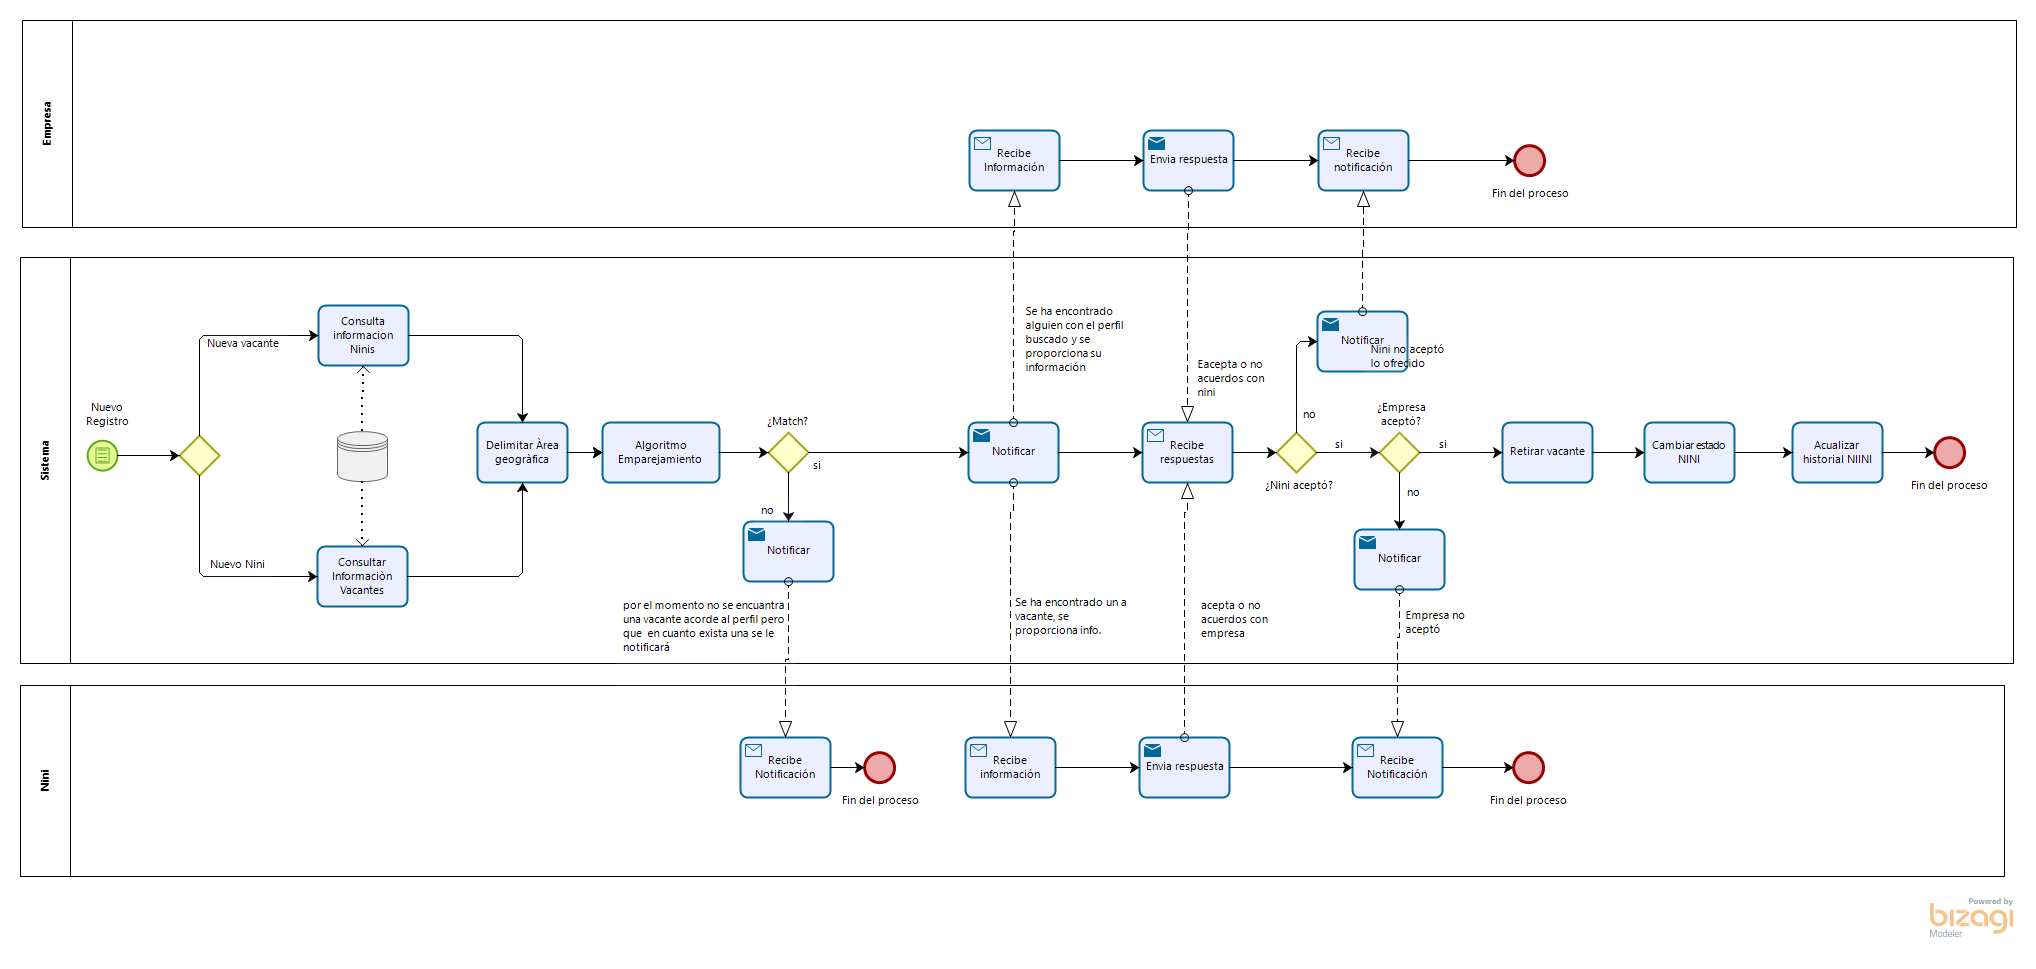
\includegraphics[angle=90, width=0.45\textwidth]{marcoTeorico/imagenes/Proceso-Asignacion.png}
                    \caption{Proceso ``Asignación''}
                    \label{ProcesoAsignacion}
                \end{center}
            \end{figure}



%\textbf{Tabla de Elementos del proceso}

%\begin{table}[htb]
%\centering
%\begin{tabular}{|l|l|}
%\hline
%\multicolumn{2}{|c|}{\textbf{Proceso Asignación}} \\ \hline
%\textbf{Procesos que dependen del proceso} &  Seguimiento \\ \hline


%\multirow{2}{*}{\textbf{Dependencia de otros procesos}} & Registro Ninis \\ %\cline{2-2}
%& Registro empresas \\ \hline

%\multirow{2}{3cm}{\textbf{Entradas}} & Datos nini \\ \cline{2-2}
%& Datos de vacantes \\ \hline

%\multirow{2}{3cm}{\textbf{Salidas}} & Notificaciones \\ \cline{2-2}
%& cambios de estado \\ \hline

%\multirow{2}{3cm}{\textbf{Precondiciones}} & Ninis Registrados \\ \cline{2-2}
%& vacantes registradas \\ \hline

%\multirow{2}{3cm}{\textbf{Postcondiciones}} & Retirar vacantes \\ \cline{2-2}
%& cambios de estado \\ \hline

%\end{tabular}
%\caption{Tabla de elementos.}
%\label{tabla:sencilla2}
%\end{table}





%%%%%%%%%%%%%%%%%%%%%%%%%%%%%%%%%%%%Registro Empresas
\newpage
\subsection{Proceso de registro de empresa}

\textbf{Objetivo} 

Realizar el registro de una empresa en el sistema.\\

\textbf{Diagrama} 
\begin{figure}[H]
\begin{center}
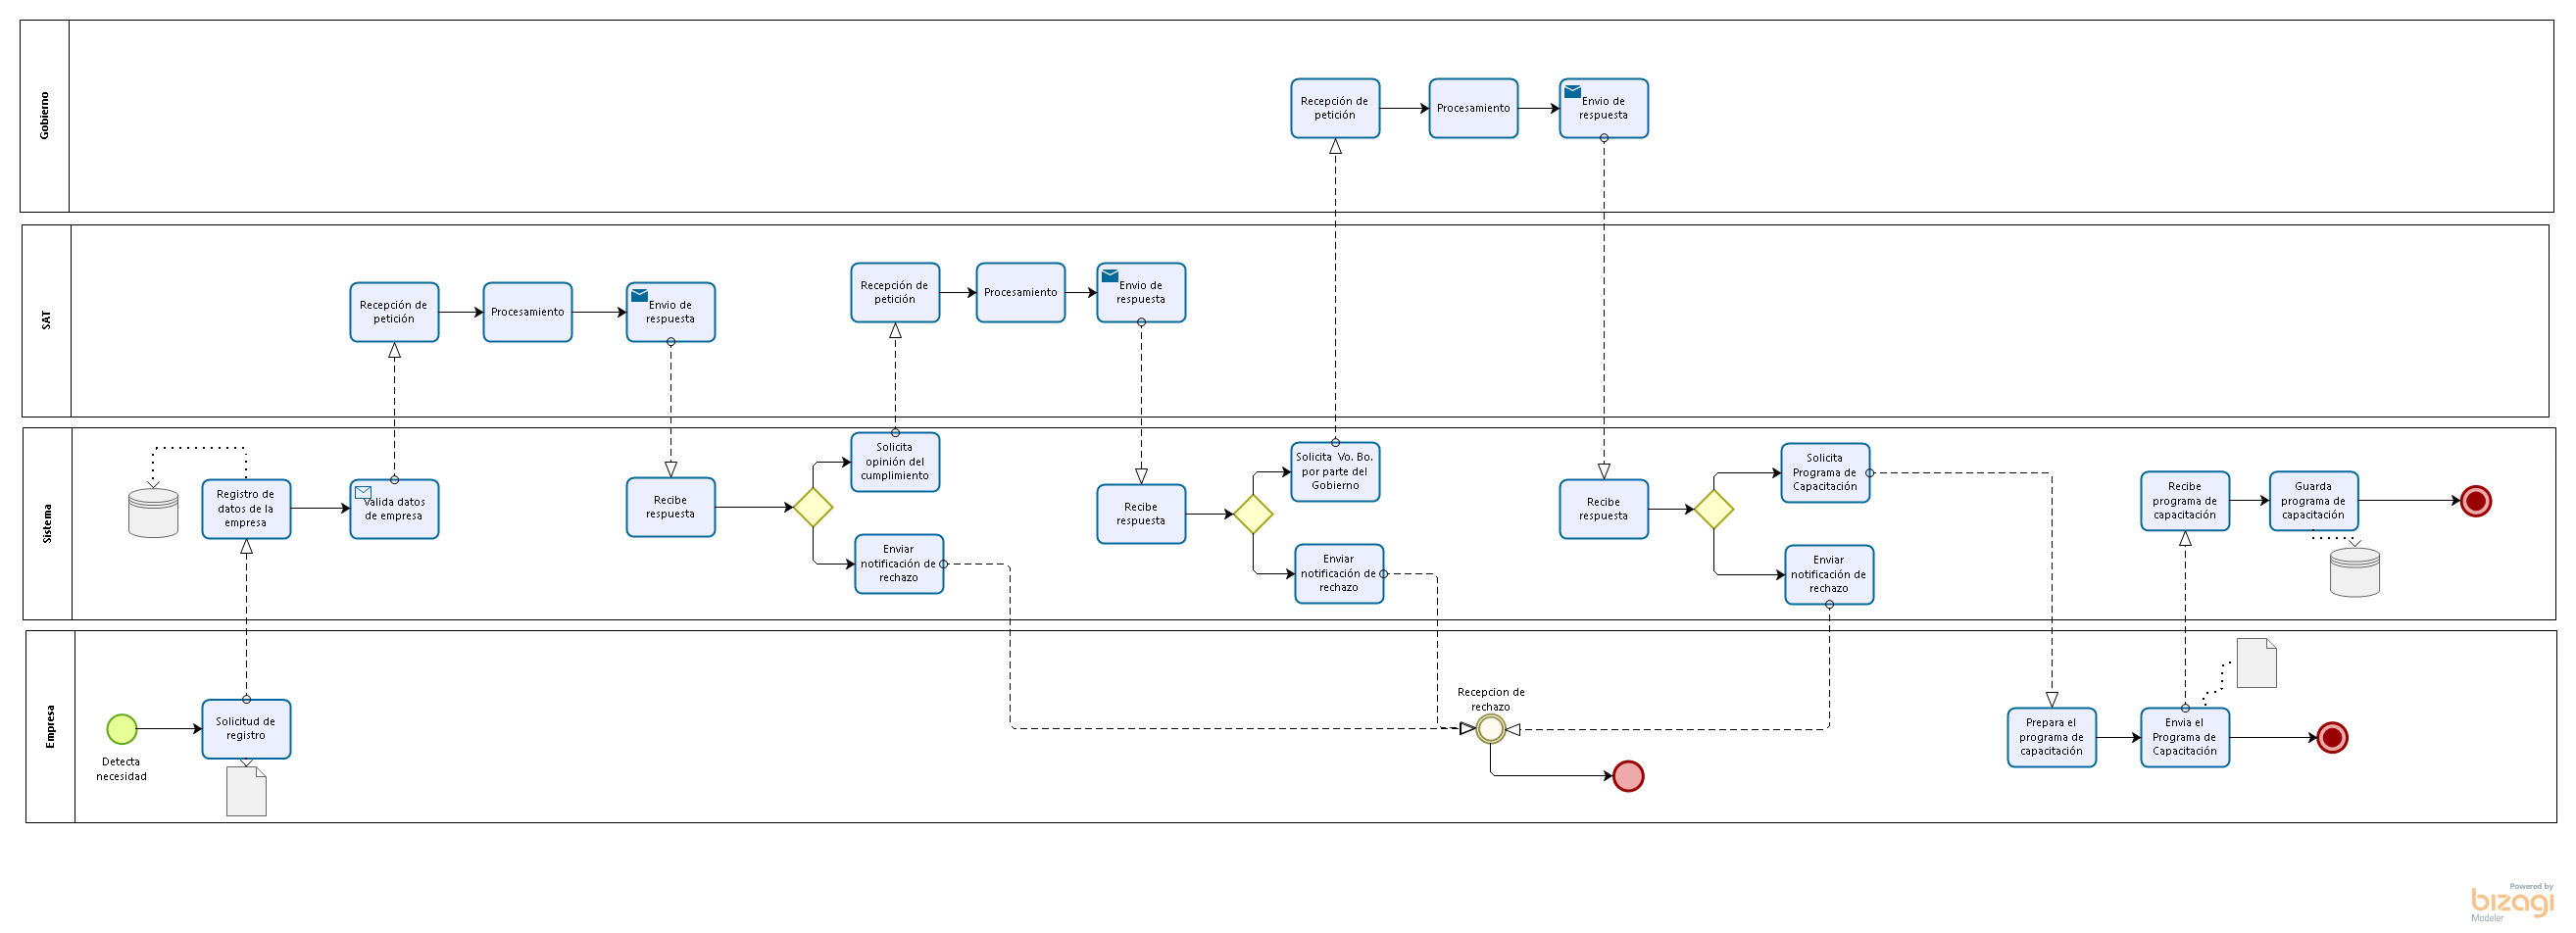
\includegraphics[angle=90, width=0.325\textwidth]{marcoTeorico/imagenes/Proceso_RegistroEmpresas.png}
\caption{Proceso ``Registro de empresa''}
\end{center}
\end{figure} 

\textbf{Descripción} \\

El proceso empieza cuando una empresa detecta una necesidad y requiere contratar personal, la empresa procede a realizar una solicitud de registro al sistema para lo cual ingresará su información y anexa los documentos que acreditan su registro como empresa (Cédula de identificación fiscal) y los documentos que permitan validar la identidad del representante de la empresa si es una persona moral o los documentos que avalen su propia identidad en caso de ser una persona física, una vez realizado esto se procede a realizar peticiones a servicios web (que serán simulados) para validar la información de la empresa con el SAT (Servicio de Administración Tributaria) para verificar el registro y conocer la “Opinión del cumplimiento”. Si la empresa cumple con la normatividad del SAT se procede a pedir el visto bueno del gobierno con la simulación del servicio web de la STPS (Secretaría del Trabajo y Previsión Social) para verificar la identidad del representante con la finalidad de continuar con el proceso.\\ \\
Después del visto bueno por parte del gobierno se solicita a la empresa su programa de capacitación para que se valide y guarde en la base de datos. \\

%\textbf{Tabla de Elementos del proceso}
%\begin{table}[htb]
%\centering
%\begin{tabular}{|l|l|}
%\hline
%\multicolumn{2}{|c|}{\textbf{Proceso Registro de Empresa}} \\ \hline
%\textbf{Procesos que dependen del proceso} &  Asignación \\ \hline

%\textbf{Dependencia de otros procesos} &  \\  \hline

%\multirow{2}{3cm}{\textbf{Entradas}} & Datos de la empresa \\ \cline{2-2}
%& Documentos para validar información \\ \hline

%\textbf{Salidas} & Notificaciones \\ \hline

%\textbf{Precondiciones} &  \\ \hline

%\textbf{Postcondiciones} & Empresa registrada \\ \hline

%\end{tabular}
%\caption{Tabla de elementos.}
%\label{tabla:sencillaEmpresas}
%\end{table}




%%%%%---------------------REGISTRO PERSONA

\newpage
\subsection{Proceso registro de becario}

\textbf{Objetivo} 

Realizar el registro de un becario en el sistema.\\
\newpage
\textbf{Diagrama} 
\begin{figure}[H]
\begin{center}
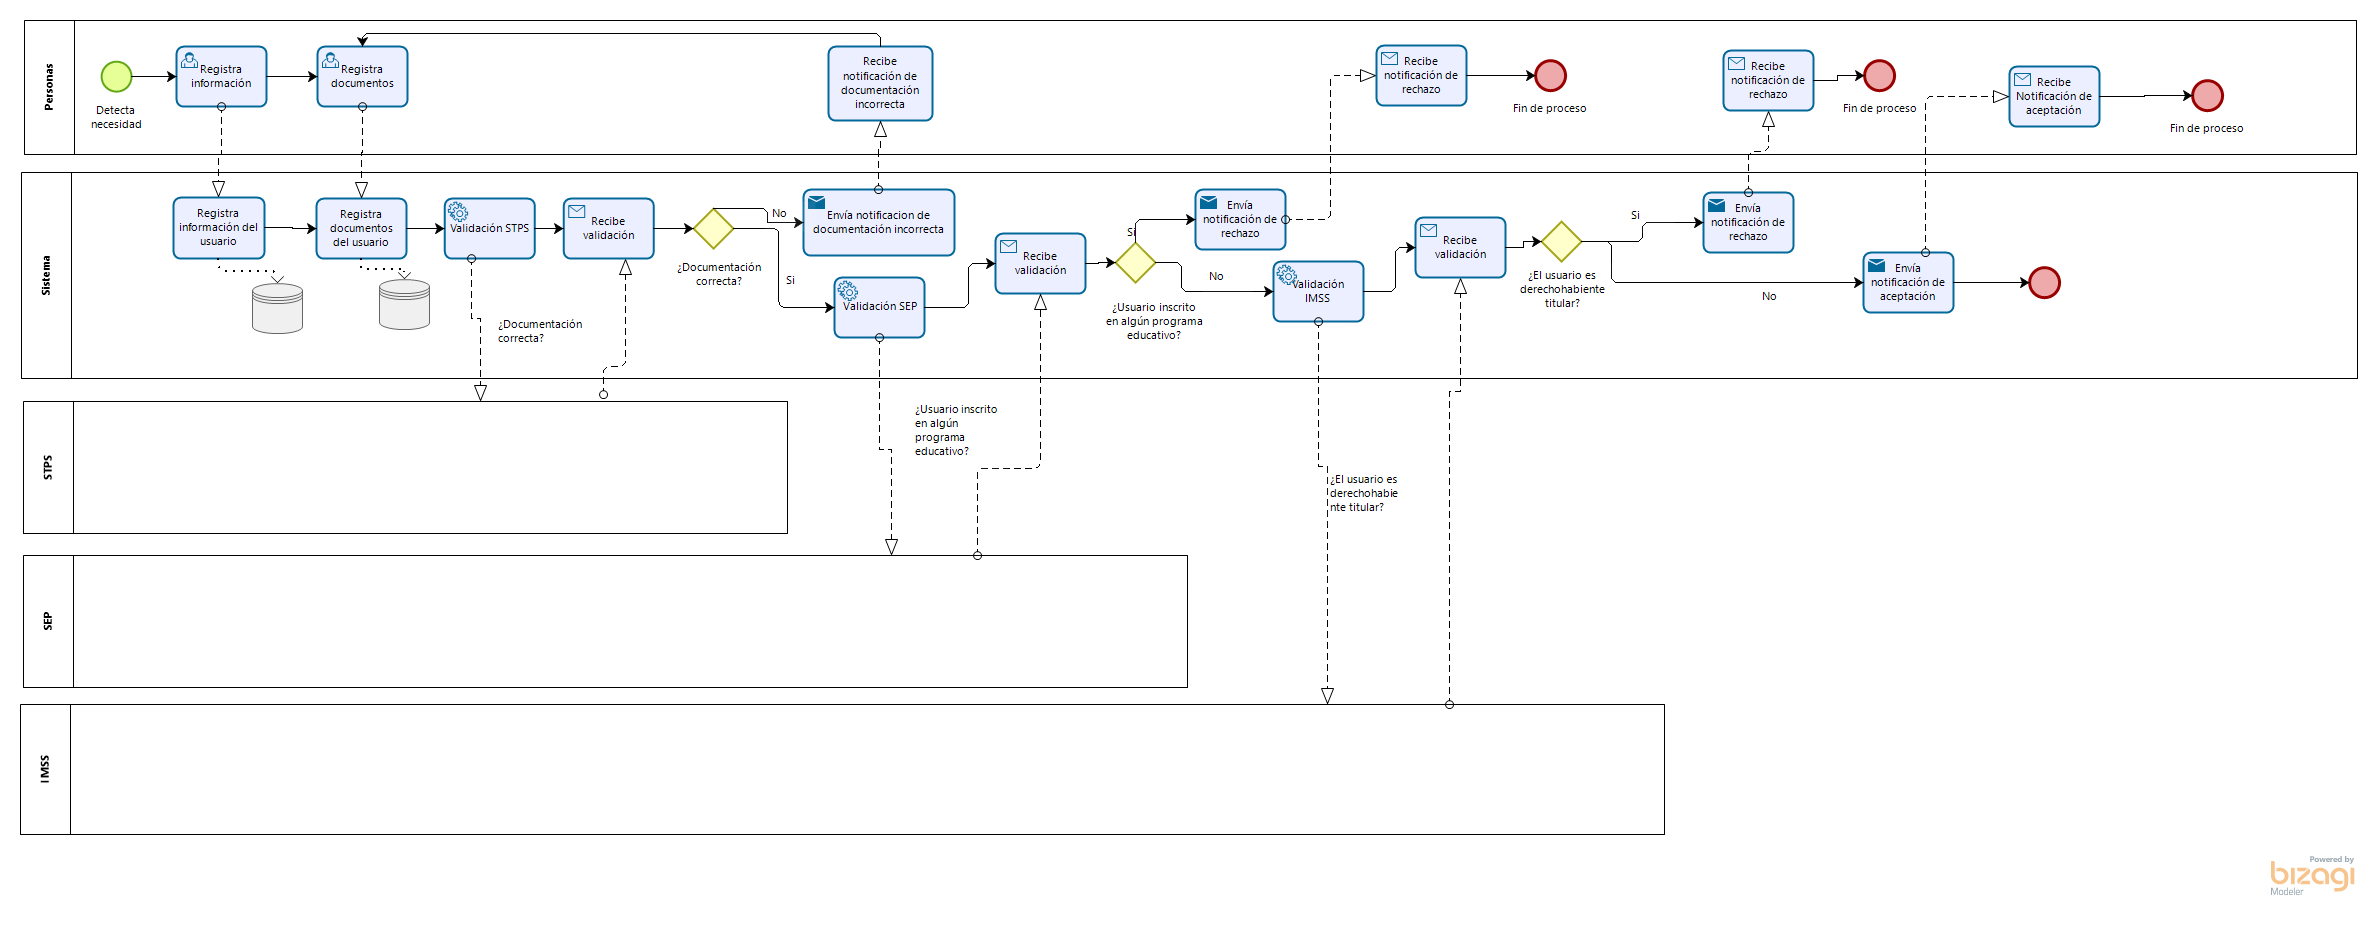
\includegraphics[angle=90,  width=0.4\textwidth]{marcoTeorico/imagenes/Proceso_RegistroPersonas.png}
\caption{Proceso ``Registro de persona''}
\end{center}
\end{figure}

\textbf{Descripción} \\

El proceso comienza cuando un becario (en este caso un NINI) detecta la necesidad de incorporarse al campo laboral, el usuario becario realiza una solicitud de registro al sistema, ingresa su información y anexa los documentos que validan su identidad y la información registrada. Ya que el sistema almacena la información, una vez que los documentos se encuentran registrados se comienza la validación con los servicios web simulados, los cuales se encargan de validar la información.\\
\\Los servicios web simulados son el de la SEP( Secretaria de Educación Pública), el del IMSS (Instituto Mexicano del Seguro Social) y la STPS (Secretaría del Trabajo y Prevención Social), una vez que se valida la información por medio de los servicios web, el sistema procede a asignarle el estado de aceptación o de rechazo al usuario. %se validan los documentos con la secretaria del Trabajo y Prevención Social (STPS) la cual valida los documentos, si los documentos son válidos 
%se procede a realizar peticiones a servicios web  que simularán la validación de la información del usuario con la SEP y el IMSS, dependiendo de la respuestas de los servicios se asigna el estado de aceptación o rechazo al usuario, una vez que el usuario es aceptado se registra en el sistema el estatus del NINI. %finalmente se ejecuta el subproceso de perfilamiento y se registra el perfil del NINI \\
\\


%\textbf{Tabla de Elementos del proceso}

%\begin{table}[htb]
%\centering
%\begin{tabular}{|l|l|}
%\hline
%\multicolumn{2}{|c|}{\textbf{Proceso Registro de Persona}} \\ \hline
%\textbf{Procesos que dependen del proceso} &  Asignación \\ \hline

%\textbf{Dependencia de otros procesos} & Proceso de perfilamiento  \\  \hline

%\multirow{2}{3cm}{\textbf{Entradas}} & Datos del NINI \\ \cline{2-2}
%& Documentos para validar información \\ \hline

%\textbf{Salidas} & Notificaciones \\ \hline

%\textbf{Precondiciones} &  \\ \hline

%\textbf{Postcondiciones} & Persona registrada \\ \hline

%\end{tabular}
%\caption{Tabla de elementos Registro de persona.}
%\label{tabla:sencillaPersonas}
%\end{table}



    %=======================================
    % Capitulo Actores
    %=========================================================
\chapter{Actores del sistema}
\label{cap:actores}
En el presente capítulo se definen los actores que participan en el sistema.\\

\IUfig[.7]{./images_Gen/Actores.png}{Actores}

\newpage
%---------------------------------------------------------
% Actor - ADMINISTRADOR  
\begin{Actor}{\hypertarget{Actor: Administrador}{\section{Administrador}}}{
	Individuo que forma parte del recurso humano del sistema, se encarga de implementar, configurar, mantener, controlar, documentar y asegurar el funcionamiento del mismo.
}
\begin{list}{}{}
    \item[Area:] \ISenter
    \begin{itemize}
		\item Administración.
    \end{itemize}
    \item[Reponsabilidades:] \ISenter
    \begin{itemize}
		\item Dar mantenimiento al sistema.
		\item Administrar usuarios.
		\item Monitorear la información ingresada por los usuarios.
		\item Mantenimiento de la documentación.
		\item Brindar soporte técnico a usuarios.
		\item Utilizar los datos personales a los que tenga acceso, en virtud de sus funciones, únicamente para el desempeño de la actividad laboral.
        \item Guardar el secreto y la confidencialidad de toda la información a la que tenga acceso.
        \item Abstenerse de borrar, destruir, dañar, alterar o modificar cualquier información relacionada con datos personales contenidos en los sistemas de información sin la autorización expresa del responsable del fichero, salvo que le haya sido asignada dicha función.
        \item Abstenerse de realizar copias, transmisiones, comunicaciones o cesiones de cualquier información relacionada con datos de carácter personal contenidos en los sistemas de información sin la autorización expresa del responsable del fichero, salvo que le haya sido asignada dicha función.

 

    \end{itemize}
%    \item[Perfil:] \ISenter
%    \begin{itemize}
%		\item Conocer los lineamientos del sistema para todos los usuarios.
%    \end{itemize}
%    \item[Cantidad:] \ISenter
%    \begin{itemize}
%		\item 1 administrador.
%    \end{itemize}
\end{list}
\end{Actor}

\newpagehttps://www.overleaf.com/8842229772jdyzmtxxsswm
%---------------------------------------------------------
% Actor - PERSONA
\begin{Actor}{\hypertarget{Actor: Becario}{\section{Becario}}}{
	Persona que tiene el interés de registrarse en el sistema y cumple con los requisitos\cdtRef{RN1}{RN-1 Perfil de Becario} para ingresar al programa.
	
}
\begin{list}{}{}
    \item[Area:] \ISenter
    \begin{itemize}
		\item Módulo Becario
    \end{itemize}
    \item[Reponsabilidades:] \ISenter
    \begin{itemize}
        \item Ingresar información real al momento de hacer su registro.
        \item Seguir buenas prácticas de seguridad en la creación de contraseñas
        \item  Tener claro que los datos que se manejan no son propiedad del que lo hace, sino del propio interesado, quienes los cede para un determinado uso o fin.
        \item Cambiar periódicamente la contraseña de autenticación de usuario.
		\item Manetener actualizada su informcaión.
		\item Responder o atender las notificaciones del sistema.
		\item Aceptar o declinar según sea el caso de las vacantes que le sean ofrecidas.
    \end{itemize}
\end{list}
\end{Actor}

%---------------------------------------------------------
% Actor - EMPRESA Fisica y moral
% Actor - EMPRESA Fisica
\begin{Actor}{\hypertarget{Actor: Empresa}{\section{Representante de Empresa}}}{
El representante de una empresa es una persona que actúa en nombre de la misma para realizar diversos trámites. Puede asumir compromisos y tomar decisiones que serán atribuidas a la empresa. En el caso de ser una persona física puede ser el o ella misma quien represente sus intereses.
}

%Organización comercial o industrial que se dedica a fabricar objetos, dar servicios o espectáculos, vender cosas, etc.
\\\\
%{\subsection{Persona Física}}{
%Es un individuo que realiza cualquier actividad económica (vendedor, comerciante, empleado, etc.),tiene obligaciones que cumplir y derechos. 
%	\\
%}
\begin{list}{}{}
    \item[Area:] \ISenter
    \begin{itemize}
		\item Módulo de Empresa
    \end{itemize}
    \item[Reponsabilidades:] \ISenter
    \begin{itemize}
        \item Ingresar información real al momento de hacer su registro.
        \item Seguir buenas prácticas de seguridad en la creación de contraseñas
        \item  Tener claro que los datos que se manejan no son propiedad del que lo hace, sino del propio interesado, quienes los cede para un determinado uso o fin.
        \item Cambiar periódicamente la contraseña de autenticación de usuario.
		\item Manetener actualizada su informcaión.
		\item Responder o atender las notificaciones del sistema.
		\item Registrar las vacantes que desea cubrir.
		\item Administrar (Actualizar, modificar ó dar de baja) las vacantes que publica.
		\item Brindar seguimiento y retroalimentación al desempeño de los becarios.
		\item Aceptar o declinar según sea el caso de los postulantes a sus vacantes.
    \end{itemize}
\end{list}
    
%{\subsection{Persona Moral}}{
	%Una persona moral es una agrupación de individuos que se unen con un fin específico, por ejemplo, una sociedad %mercantil o una asociación civil.
%	\\
%}
%\begin{list}{}{}
%    \item[Area:] \ISenter
%    \begin{itemize}
%		\item n/a.
 %   \end{itemize}
  %  \item[Reponsabilidades:] \ISenter
   % \begin{itemize}
%		\item Registrarse en el programa y manetener actualizada su informcaión para poder ofrecer vacantes.
    %\end{itemize}
    %\item[Perfil:] \ISenter
%    \begin{itemize}
%		\item Estar reguladas por la ley.
%		\item Cumplir con todas sus obligaciones con el SAT
 %   \end{itemize}
 %   \item[Cantidad:] \ISenter
%    \begin{itemize}
%		\item 1 representante por empresa.
%    \end{itemize}
%\end{list}
\end{Actor}




    %=======================================
    % Capitulo Requerimientos del sistema
    \chapter{Requerimientos del sistema}
\label{cap:reqSist}

\section{Notación, símbolos y convenciones utilizadas}

	Los requerimientos funcionales utilizan una clave RFX, donde:
	
\begin{description}
	\item[RFS] Es la clave para todos los {\bf R}equerimientos {\bf F}uncionales del {\bf S}istema.
	\item[RFU] Es la clave para todos los {\bf R}equerimientos {\bf F}uncionales del {\bf U}suario.
	\item[RFA] Es la clave para todos los {\bf R}equerimientos {\bf F}uncionales del {\bf A}dministrador.
	\item[X] Es un número consecutivo: 1, 2, 3, ...
\end{description}

	Además, para los requerimientos funcionales se usan las abreviaciones que se muestran en la tabla~\ref{tbl:leyendaRF}.
\begin{table}[hbtp!]
	\begin{center}
    \begin{tabular}{|r l|}
	    \hline
    	{\footnotesize Id} & {\footnotesize\em Identificador del requerimiento.}\\
    	{\footnotesize Pri.} & {\footnotesize\em Prioridad}\\
    	{\footnotesize Ref.} & {\footnotesize\em Referencia a los Requerimientos de usuario.}\\
    	{\footnotesize MA} & {\footnotesize\em Prioridad Muy Alta.}\\
    	{\footnotesize A} & {\footnotesize\em Prioridad Alta.}\\
    	{\footnotesize M} & {\footnotesize\em Prioridad Media.}\\
    	{\footnotesize B} & {\footnotesize\em Prioridad Baja.}\\
    	{\footnotesize MB} & {\footnotesize\em Prioridad Muy Baja.}\\
		\hline
    \end{tabular} 
    \caption{Leyenda para los requerimientos funcionales.}
    \label{tbl:leyendaRF}
	\end{center}
\end{table}

\newpage

\section{Requerimientos funcionales}
Los requerimiento funcionales describen lo que el sistema debe hacer.\\

Son declaraciones de los servicios que debe proporcionar el sistema, de la manera en que éste debe reaccionar con determinadas entradas y situaciones, también pueden declarar lo que el sistema no debe hacer \cite{Req}

\begin{table}[htbp!]
	\begin{requerimientos}
	    \FRitem{RFS1}{Inicio de sesión}{El sistema permitirá el manejo de distintos tipos de sesiones de acuerdo al tipo de usuario.}{A}{RU}
	    \FRitem{RFS2}{Registro de becarios}{El sistema permitirá el registro, consulta, actualización y eliminación de los usuarios \cdtRef{Actor: Becario}{Becario} con el fin de tener registro de los solicitantes.}{A}{RU}
	   	\FRitem{RFS3}{Registro de empresas}{El sistema permitirá el registro, consulta, actualización y eliminación las \cdtRef{Actor: Empresa}{Empresa} que se encuentren ofertando vacantes.}{A}{RU}
		\FRitem{RFU1}{Registro de vacantes}{El usuario desea registrar, consultar, actualizar y eliminar vacantes ofertadas.}{A}{RU}

		\FRitem{RFA1}{Gestionar usuarios}{El administrador desea gestionar y visualizar la informacion de los usuario registrados en el sistema.}{A}{RU}
		\FRitem{RFA2}{Gestionar archivos}{El administrador desea gestionar los archivos registrados en el sistema.}{A}{RU}
	\end{requerimientos}
    \caption{Requerimientos funcionales.}
    \label{tb1:reqFunc}
\end{table}


\newpage

\section{Requerimientos no funcionales} 

Son restricciones de los servicios o funciones ofrecidos por el sistema. Incluyen restricciones de tiempo, proceso de desarrolloo y estándares\cite{Req}.

\begin{table}[htbp!]
	\begin{requerimientosnf}
	    %% -Requerimientos funcionales de sistema
	    \FRitem{RNF1}{Portabilidad}{El sistema estará disponible mediante una aplicacion web. Estará soportada con el siguiente navegador web:
	            \begin{itemize}
	                \item Google Chrome.
	            \end{itemize}
	            Según las estadisticas de \cite{statcounter} el 63.72 \% de los usuarios utilizan Chrome para navegar, a demás que es soportado por Linux, Windows, etc.
	            \newline
	            Como versión utilizaremos la mas reciente a la que estamos realizando el TT (Versión 77.0.3865.90).
	        }{A}{RU}
	    %ado hasta por 400 usuario, (se comprobará a través de pruebas de estrés) siempre y cuando se tenga una conexion estable a Internet.}{A}{RU}
	    \FRitem{RNF2}{Fiabilidad}{
	        \begin{itemize}
	            \item El sistema deberá trabajar de manera correcta bajo condiciones de uso especificadas en los Caosos de Uso.
	            \item El sistema trabajará correctamente con una conexión estable a internet.
	            \item No debe haber perdida de información cuando se realiza una transacción y haya una falla en el servidor.
	        \end{itemize}
	        %aqui estaba lo de no exigir de más al sistema
	       
	        Nota: Se refiere condición estable cuando tenemos conexión a internet con un ancho de banda mayor a 1000 kb/s por medio de cable Ethernet, sin ningun tipo de fallo de hardware.}{A}{RU}
		\FRitem{RNF3}{Mantenibilidad}{Todo el sistema estará documentado y estructurado.
		\newline
		Procesos, cosos de uso y código estructurados de una manera consistente e integral (con la documentación correspondiente) previendo la facilidad del mantenimiento a futuro.}{A}{RU}
		
	\end{requerimientosnf}
    \caption{Requerimientos no funcionales del sistema.}
    \label{tb2:reqNoFunc}
\end{table}
 %Nota: Se considera condición normal las consultas o las transacciones que pueda realizar.
%	        \newline
\newpage
%%--------------
\subsection{Restricciones de construcción}
\begin{table}[htbp!]
	\begin{restcon}
	    %% -Requerimientos funcionales de sistema
	    \RCitem{RC1}{Manejador de Base de Datos}{El sistema usa el  manejado de base de datos MySQL.}
	    \RCitem{RC2}{Sistema Operativo del servidor}{El servidor esta montado en Google Cloud con un SO Windows Server 2012.}
	    \RCitem{RC3}{Memoria RAM del servidor}{El servidor tiene una memoria RAM de 16384 MB.}
	    \RCitem{RC4}{CPU del servidor}{El servidor tiene un CPU Dual 2.8 GHz Intel Xenon(R) (Hyper-Threaded).}
		\RCitem{RC5}{Sistema Operativo en el sistema}{Al utilizar Google Chrome podemos asegurar que podra utilizar el sistema en cuelaquier Sistema Operativo. }
		
\end{restcon}
    \caption{Restricciones de construcción del sistema.}
    \label{tb3:RestriccionesDeConstruccion}
\end{table}

    
    %=======================================
    % Capitulo Reglas del negocio
    %=========================================================
\chapter{Reglas del Negocio}
\label{cap:reglasNegocio}

Las reglas de negocio son directivas que tienen como fundamento la misión de un negocio y como objetivo regir estrategias para poder conseguir esta misión. Una regla de negocio no requiere de una interpretación adicional. Estas reglas también son una fuente de información muy relevante ya que generalmente establecen las relaciones entre dos o más términos del negocio.

En el documento se presentarán estas reglas en forma de secciones indicando los siguientes atributos:

\begin{itemize}
    \item \textbf{Id:} Es el identificador de la regla de negocio con la cual se podrá referenciar a lo largo del documento.
    \item \textbf{Nombre:} Indica el nombre de la regla de negocio el cual debe describir de forma concisa en qué consiste la regla.
    \item \textbf{Tipo:} Indica el tipo de regla de negocio de acuerdo a como se aplica.
        \begin{itemize}
            \item \textbf{Habilitadora:} Permite realizar el proceso en el que la regla se ve involucrada.
            \item \textbf{Cronometrada:} Recibe parámetros y con respecto a eso realiza el proceso.
            \item \textbf{Ejecutiva:} Es aquella que se debe llevar a cabo cuando una autoridad se ve involucrada para que el proceso concluya.
        \end{itemize}
    \item \textbf{Clase:} Indica la naturaleza de la regla de negocio.
        \begin{itemize}
            \item \textbf{Condición:} Es una regla que cumple una condición para llevarse a cabo.
            \item \textbf{Integridad:} Es una regla que indica validaciones que, de no ser tomadas en cuenta se pone en peligro la integridad de la informacion.
            \item \textbf{Autorización:} Son restricciones en las que se ven involucradas palabras como, al menos uno.
        \end{itemize} 
    \item \textbf{Nivel:} Indica cómo es que la regla se toma en cuenta para el desarrollo del sistema.
        \begin{itemize}
            \item \textbf{Controla:} Define que el sistema se encargará de vigilar el cumplimiento de la regla en todo momento.
            \item \textbf{Influencia:} Sugiere formas en las que se debe realizar la operación, pero no la limita. De tal forma que el sistema dará facilidades para evitar esas situaciones o advertirá cada vez que se detecte que la regla no es tomada en cuenta.
        \end{itemize}
    \item \textbf{Descripción:} Es un pequeño resumen que ayuda a entender la regla de negocio.
    \item \textbf{Motivación:} La razón detrás de la existencia de la regla de negocio.
    \item \textbf{Sentencia:} Descripción formal o matemática de la regla de negocio.
\end{itemize}


%%Aqui van los inputs a las reglas de negocio

%   Regla de negocio Mario
%   - RFC
%   - CURP (Personas) 

%
% Regla del Negocio #1 - Perfil de becario
%-----------------------------------------------
\section{Regla de Negocio 1.- Perfil de Becario}

\begin{BussinesRule}{RN1}{Perfil de Becario}
	\BRitem[Tipo:] Regla de restricción (Validación).
				% Otras opciones para tipo: 
				% - Regla de integridad referencial o estructural. 
				% - Regla de operación, (calcular o determinar un valor.).
				% - Regla de inferencia de un hecho.
	\BRitem[Clase:] Habilitadora. 
				% Otras opciones para clase: Habilitadora, Cronometrada, Ejecutiva.
	\BRitem[Nivel:] Control. % Otras opciones para nivel: Control, Influencia.
	\BRitem[Descripción:] Un becario es aquel usuario registrado en el sistema que no estudia ni trabaja.
	\BRitem[Motivación:] Tener únicamente registrados a las personas que cumplan con:
	\begin{itemize}
	    \item No estudiar.
	    \item No trabajar.
	\end{itemize}
	
\end{BussinesRule}



%========================================================
%========================================================
% Regla del Negocio #2 - Campo obligatorio
%-----------------------------------------------
\section{Regla de Negocio 2.- Campo obligatorio}

\begin{BussinesRule}{RN2}{Campo obligatorio}
	\BRitem[Tipo:] Regla de restricción (Validación).
				% Otras opciones para tipo: 
				% - Regla de integridad referencial o estructural. 
				% - Regla de operación, (calcular o determinar un valor.).
				% - Regla de inferencia de un hecho.
	\BRitem[Clase:] Habilitadora. 
				% Otras opciones para clase: Habilitadora, Cronometrada, Ejecutiva.
	\BRitem[Nivel:] Control. % Otras opciones para nivel: Control, Influencia.
	\BRitem[Descripción:] Los campos de este formulario que contienen al inicio un * no pueden ser un campo vacío.
	\BRitem[Motivación:] Tener los datos correspondientes para validar el campo en el sistema. 
\end{BussinesRule}

%========================================================
% Regla del Negocio #3 - Formato de CURP
%-----------------------------------------------
\section{Regla de Negocio 3.- Formato de CURPs}

\begin{BussinesRule}{RN3}{Formato de CURP}
	\BRitem[Tipo:] Regla estructural. 
				% Otras opciones para tipo: 
				% - Regla de integridad referencial o estructural. 
				% - Regla de operación, (calcular o determinar un valor.).
				% - Regla de inferencia de un hecho.
	\BRitem[Clase:] Habilitadora. 
				% Otras opciones para clase: Habilitadora, Cronometrada, Ejecutive.
	\BRitem[Nivel:] Control. % Otras opciones para nivel: Control, Influencia.
	\BRitem[Descripción:] La Clave Única de Registro de Población (CURP) es un instrumento de registro que se asigna a todas las personas que viven en el territorio nacional, así como a los mexicanos que residen en el extranjero\cite{SG}. La instancia responsable de asignar la CURP y de expedir la Constancia respectiva es el Registro Nacional de Población.\\
	El CURP está integrado con dieciocho elementos, representados por letras y números, que se generan a partir de los datos contenidos en el documento probatorio de tu identidad como acta de nacimiento, carta de naturalización o documento migratorio \cite{SG}, y que se refieren a:
	        \begin{itemize}
	            \item El primer apellido, segundo apellido y nombre de pila.
	            \item La fecha de nacimiento.
	            \item El sexo.
	            \item La entidad federativa de nacimiento.
	            \item Los dos últimos elementos de la CURP evitan la duplicidad de la Clave y garantizan su correcta integración.
	           
	        \end{itemize}
	        
	
	\BRitem[Motivación:] Registrar en el sistema CURPs con estructuras correctas.
	\BRitem[Sentencia:] $\forall\ x \in CURP \Rightarrow  [A-Z]{4}[0-9]{6}[H|M][A-Z]{5}[0-9]{2}$
	\BRitem[Ejemplo positivo:] Cumplen la regla de negocio los siguientes CURPs:
        \begin{itemize}
			\item OORE970504MMCSDS03
			\item OORI061120MMCSDS19
        \end{itemize}
	\BRitem[Ejemplo negativo:] No cumplen la regla de negocio los siguientes CURPs.
		\begin{itemize}
        	\item OORE9705MMCSDS03
			\item OORI061120M82SDSKL
        	
    \end{itemize}
\end{BussinesRule}





%========================================================
% Regla del Negocio #4 - Formato de NSS
%-----------------------------------------------
\section{Regla de Negocio 3.- Formato de Número de Seguro Social }

\begin{BussinesRule}{RN3}{Formato de Número de Seguro Social (NSS)}
	\BRitem[Tipo:] Regla estructural. 
				% Otras opciones para tipo: 
				% - Regla de integridad referencial o estructural. 
				% - Regla de operación, (calcular o determinar un valor.).
				% - Regla de inferencia de un hecho.
	\BRitem[Clase:] Habilitadora. 
				% Otras opciones para clase: Habilitadora, Cronometrada, Ejecutiva.
	\BRitem[Nivel:] Control. % Otras opciones para nivel: Control, Influencia.
	\BRitem[Descripción:]El Número de Seguro Social (NSS) es un número compuesto de once (11) dígitos con el cual los trabajadores que cotizan en el IMSS son identificados por dicha institución desde el mismo momento de su afiliación. Es de carácter personal, permanente y único \cite{NSS}. Su secuencia de números se compone de los siguientes elementos:
	        \begin{itemize}
	            \item Los dos primeros dígitos Refiere a la subdelegación en el que fue afiliado
	            \item Tercer y cuarto digito corresponden al año de afiliación
	            \item Quinto y sexto digito se refieren a la fecha de nacimiento del afiliado.
	            \item Los siguientes cuatro dígitos son los que el IMSS le asignado al trabajador.
	            \item El último digito es el número de verificación del trabajador ante el IMSS.
	           
	        \end{itemize}
	        
	
	\BRitem[Motivación:] Registrar en el sistema NSSs con estructuras correctas.
	\BRitem[Sentencia:] $\forall\ x \in NSS \Rightarrow     [0-9]{11}$
	\BRitem[Ejemplo positivo:] Cumplen la regla de negocio los siguientes NSSs:
        \begin{itemize}
			\item 14567892345
			\item 98547928354
        \end{itemize}
	\BRitem[Ejemplo negativo:] No cumplen la regla de negocio los siguientes NSSs.
		\begin{itemize}
        	\item 8654935
			\item 67435GTJ2
        	
    \end{itemize}
\end{BussinesRule}


%========================================================
% Regla del Negocio #5 - Adjuntar un archivo 
%-----------------------------------------------
\section{Regla de Negocio 5.- Adjuntar un archivo válido}

\begin{BussinesRule}{RN5}{Adjuntar un archivo válido}
%\label{BR:RN5}
	\BRitem[Tipo:] Regla de integridad. 
				% Otras opciones para tipo: 
				% - Regla de integridad referencial o estructural. 
				% - Regla de operación, (calcular o determinar un valor.).
				% - Regla de inferencia de un hecho.
	\BRitem[Clase:] Habilitadora. 
				% Otras opciones para clase: Habilitadora, Cronometrada, Ejecutive.
	\BRitem[Nivel:] Control. % Otras opciones para nivel: Control, Influencia.
	\BRitem[Descripción:] Al adjuntar un archivo este solo será recibido por el sistema si está en el formato PDF.
	\BRitem[Motivación:] Evitar que se guarden en el sistema archivos que no requiera el sistema para el registro de becarios.
	\BRitem[Sentencia:] 
	   Se tiene a un becario que desea adjuntar sus documentos para registrarse en el sistema.
	\BRitem[Ejemplo positivo:] El usuario adjunta su archivo de CURP ``CURP.pdf''.
	
	\BRitem[Ejemplo negativo:] El usuario adjunta su archivo de CURP ``CURP.xml''. 
\end{BussinesRule}
%========================================================
% Regla del Negocio #6 - Tamaño de archivo incorrecto
%-----------------------------------------------
\section{Regla de Negocio 6.- Tamaño de archivo incorrecto}
\begin{BussinesRule}{RN6}{Tamaño de archivo incorrecto}

	\BRitem[Tipo:] Regla de integridad referencial o estructural. 
				% Otras opciones para tipo: 
				% - Regla de integridad referencial o estructural. 
				% - Regla de operación, (calcular o determinar un valor.).
				% - Regla de inferencia de un hecho.
	\BRitem[Clase:] Habilitadora. 
				% Otras opciones para clase: Habilitadora, Cronometrada, Ejecutive.
	\BRitem[Nivel:] Control. % Otras opciones para nivel: Control, Influencia.
	\BRitem[Descripción:]	Los archivos adjuntos deben tener un tamaño límite de 5 MB. 
	\BRitem[Motivación:] Evitar archivos de peso excesivo que puedan alentar el funcionamiento del sistema.
	\BRitem[Sentencia:]
	    Sea x un archivo.jpg y n el tamaño que puede tener el archivo x, entonces n es menor o igual a 3 MB.

	\BRitem[Ejemplo positivo:] Archivo con tamaño dentro del rango permitido:		
        \begin{itemize}
        	\item Archivo.jpg (3 MB)
			\item Archivo2.jpg (1.5 MB)
        \end{itemize}
	
	\BRitem[Ejemplo negativo:] Archivo con tamaño excedente del rango permitido:
		\begin{itemize}
        	\item Archivo.jpg (176 MB)
			\item Archivo2.jpg (20 MB)
        \end{itemize}
	%\BRitem[Referenciado por:] \hyperlink{CUCE3.2}{CUCE3.2}, \hyperlink{CUCE3.3}{CUCE3.3}.
\end{BussinesRule}


%========================================================
% Regla del Negocio #7 - Formato de CP
%-----------------------------------------------
\section{Regla de Negocio 7.- Formato de Código Postal}

\begin{BussinesRule}{RN7}{Formato de Código Postal}
	\BRitem[Tipo:] Regla estructural. 
				% Otras opciones para tipo: 
				% - Regla de integridad referencial o estructural. 
				% - Regla de operación, (calcular o determinar un valor.).
				% - Regla de inferencia de un hecho.
	\BRitem[Clase:] Habilitadora. 
				% Otras opciones para clase: Habilitadora, Cronometrada, Ejecutiva.
	\BRitem[Nivel:] Control. % Otras opciones para nivel: Control, Influencia.
	\BRitem[Descripción:]Clave numérica compuesta por cinco dígitos que identifica y ubica un área geográfica del país y la oficina postal que la sirve, para facilitar al correo, el encaminamiento, la distribución y el reparto de la materia postal \cite{CP}. Su denominación abreviada será C.P.

	\BRitem[Motivación:] Registrar en el sistema CPs con estructuras correctas.
	\BRitem[Sentencia:] $\forall\ x \in CP \Rightarrow   [0-9]{1}[1-9]{1}[0-9]{3}$
	\BRitem[Ejemplo positivo:] Cumplen la regla de negocio los siguientes CPs:
        \begin{itemize}
			\item 57630
			\item 45678
        \end{itemize}
	\BRitem[Ejemplo negativo:] No cumplen la regla de negocio los siguientes CP:
		\begin{itemize}
        	\item 00564
			\item O54t6
        	
    \end{itemize}
\end{BussinesRule}




%========================================================
% Regla del Negocio #8 - Formato de RFC
%-----------------------------------------------
\section{Regla de Negocio 8.- Formato de Registro Federal de Contribuyentes}

\begin{BussinesRule}{RN8}{Formato de Registro Federal de Contribuyentes }
	\BRitem[Tipo:] Regla estructural. 
				% Otras opciones para tipo: 
				% - Regla de integridad referencial o estructural. 
				% - Regla de operación, (calcular o determinar un valor.).
				% - Regla de inferencia de un hecho.
	\BRitem[Clase:] Habilitadora. 
				% Otras opciones para clase: Habilitadora, Cronometrada, Ejecutiva.
	\BRitem[Nivel:] Control. % Otras opciones para nivel: Control, Influencia.
	\BRitem[Descripción:]El RFC es una clave que identifica como contribuyentes a las personas físicas o morales en México para controlar el pago de impuestos frente al SAT, el Servicio de Administración Tributaria \cite{RFC}. Su denominación abreviada será RFC y esiten dos tipos, el RC para personas físicas y para personas morales o empresas.
	\begin{itemize}
	            \item Personas físicas:
	            \begin{itemize}
	                \item Primera letra y primera vocal interna del primer apellido
                    \item Primera letra del segundo apellido
                    \item Primera letra del primer nombre del contribuyente
                    \item Fecha de nacimiento en formato aa/mm/dd
                    \item Homoclave calculada con un algoritmo de público conocimiento, con dígito verificador para evitar repeticiones (asignado por el SAT)
	            \end{itemize}
	            \item Personas morales:
	            \begin{itemize}
	                \item Si el nombre de la empresa tiene tres palabras, usar la primera letra de cada una. Si tiene dos, usar la primera de la primer palabra, y las primeras dos de la segunda. Si tiene una, usar sus primeras tres letras.
                \item Fecha de constitución de la empresa en formato aa/mm/dd
                \item Homoclave (asignada por el SAT)
	            \end{itemize}
	        \end{itemize}

	\BRitem[Motivación:] Registrar en el sistema RFCs con estructuras correctas.
	\BRitem[Sentencia:]  $\forall\ x \in RFC \Rightarrow   ([A-Z,\tilde{N},\&]{3,4}([0-9]{2})(0[1-9]|1[0-2])(0[1-9]|1[0-9]|2[0-9]|3[0-1])[A-Z0-9]{3})$
	\BRitem[Ejemplo positivo:] Cumplen la regla de negocio los siguientes RFCs:
        \begin{itemize}
			\item GOAP780710RH7
			\item IAT030120E60
        \end{itemize}
	\BRitem[Ejemplo negativo:] No cumplen la regla de negocio los siguientes RFCs.
		\begin{itemize}
        	\item G4Pu345670GGT
			\item IA6030150E60
        	
    \end{itemize}
\end{BussinesRule}




%========================================================
%========================================================
% Regla del Negocio #9 - Contraseña
%-----------------------------------------------
\section{Regla de Negocio 9.- Contraseña valida}

\begin{BussinesRule}{RN9}{Contraseña valida}
	\BRitem[Tipo:] Regla de restricción (Validación).
				% Otras opciones para tipo: 
				% - Regla de integridad referencial o estructural. 
				% - Regla de operación, (calcular o determinar un valor.).
				% - Regla de inferencia de un hecho.
	\BRitem[Clase:] Habilitadora. 
				% Otras opciones para clase: Habilitadora, Cronometrada, Ejecutiva.
	\BRitem[Nivel:] Control. % Otras opciones para nivel: Control, Influencia.
	\BRitem[Descripción:] La contraseña debera cumplir con tener una longitud mínima de 8 caracteres y máxima de 16 caracteres, contener una letra mayúscula, una minúscula, un número y un caracter especial \cite{contra}.
	\BRitem[Motivación:] Almacenar constraseñas seguras para los usuarios. 
	\BRitem[Sentencia:] $\forall\ x \in Contraseña \Rightarrow     {(?=.+[0-9])(?=.+[a-z])(?=.+[A-Z])(?=.+[\#\$\&\%@])} {8-16}$
	
		\BRitem[Ejemplo positivo:] Contraseña valida:		
        \begin{itemize}
        	\item P4s\$word
        \end{itemize}
	
	\BRitem[Ejemplo negativo:] Contraseña invaida:
		\begin{itemize}
        	\item Contraseña   
			\end{itemize}
\end{BussinesRule}

%========================================================
%========================================================
% Regla del Negocio #10 - Número de becarios
%-----------------------------------------------
\section{Regla de Negocio 10.- Número telefónico (fijo o celular)}

\begin{BussinesRule}{RN10}{Número telefónico (fijo o celular)}
	\BRitem[Tipo:] Regla de restricción (Validación).
				% Otras opciones para tipo: 
				% - Regla de integridad referencial o estructural. 
				% - Regla de operación, (calcular o determinar un valor.).
				% - Regla de inferencia de un hecho.
	\BRitem[Clase:] Habilitadora. 
				% Otras opciones para clase: Habilitadora, Cronometrada, Ejecutiva.
	\BRitem[Nivel:] Control. % Otras opciones para nivel: Control, Influencia.
	\BRitem[Descripción:] El teléfono ingresado por el usuario puede ser fijo o celular.
	\BRitem[Motivación:] Que los becarios ingresen números telefónicos validos. 
	
		\BRitem[Sentencia:] $\forall\ x \in N\'umero Tel\'efonico \Rightarrow     [0-9]{10}$
	\BRitem[Ejemplo positivo:] Cumplen la regla de negocio los siguientes Teléfonos:
        \begin{itemize}
			\item 5544678932
			\item 5432146789
        \end{itemize}
	\BRitem[Ejemplo negativo:] No cumplen la regla de negocio los siguientes Teléfonos.
		\begin{itemize}
        	\item 34875116
			\item 67435GTJ2
        	
    \end{itemize}

\end{BussinesRule}

%========================================================
%========================================================
% Regla del Negocio #11 - Datos que se pueden editar
%-----------------------------------------------
\section{Regla de Negocio 11.- Datos que se pueden editar}

\begin{BussinesRule}{RN11}{Datos que se pueden editar}
	\BRitem[Tipo:] Regla de restricción (Validación).
				% Otras opciones para tipo: 
				% - Regla de integridad referencial o estructural. 
				% - Regla de operación, (calcular o determinar un valor.).
				% - Regla de inferencia de un hecho.
	\BRitem[Clase:] Habilitadora. 
				% Otras opciones para clase: Habilitadora, Cronometrada, Ejecutiva.
	\BRitem[Nivel:] Control. % Otras opciones para nivel: Control, Influencia.
	\BRitem[Descripción:] El usuario puede editar solamente ciertos datos. En caso de que quiera editar algun dato que no se encuentre en la lista siguiente, debera acudir con el administrador del sistema.\\
	Datos que se pueden editar:
	\begin{itemize}
	    \item Becario:
	        \begin{itemize}
	            \item Télefono fijo.
	            \item Télefono celular.
	            \item Discapacidad.
	            \item Grado de estudios.
	            \item Dirección.
	            \item Documentos.
	        \end{itemize}
	   \item Empresa:
	        \begin{itemize}
	            \item Giro empresarial.
	            \item Información personal o del representante de la empresa.
	        \end{itemize}
	\end{itemize}
	\BRitem[Motivación:] Que el usuario pueda editar inormación que no pueda tener un impacto en el sistema. 

\end{BussinesRule}

%========================================================
%========================================================
% Regla del Negocio #12 - Número oficia-exterior
%-----------------------------------------------
\section{Regla de Negocio 12.- Número oficial(exterior)}

\begin{BussinesRule}{RN12}{Número oficial(exterior)}
	\BRitem[Tipo:] Regla de restricción (Validación).
				% Otras opciones para tipo: 
				% - Regla de integridad referencial o estructural. 
				% - Regla de operación, (calcular o determinar un valor.).
				% - Regla de inferencia de un hecho.
	\BRitem[Clase:] Habilitadora. 
				% Otras opciones para clase: Habilitadora, Cronometrada, Ejecutiva.
	\BRitem[Nivel:] Control. % Otras opciones para nivel: Control, Influencia.
	\BRitem[Descripción:]  El Número Oficial es la asignación alfanumérica que le corresponde a un predio en la secuencia predeterminada por cada vía pública para su correcta identificación \cite{NO}. Longitud máxima 10 dígitos. 
	\BRitem[Motivación:] Almacenar números exteriores validos. 

\end{BussinesRule}

%========================================================
%========================================================
% Regla del Negocio #12 - Número oficia-exterior
%-----------------------------------------------
\section{Regla de Negocio 13.- Correo electrónico}

\begin{BussinesRule}{RN13}{Correo electrónico}
	\BRitem[Tipo:] Regla de restricción (Validación).
				% Otras opciones para tipo: 
				% - Regla de integridad referencial o estructural. 
				% - Regla de operación, (calcular o determinar un valor.).
				% - Regla de inferencia de un hecho.
	\BRitem[Clase:] Habilitadora. 
				% Otras opciones para clase: Habilitadora, Cronometrada, Ejecutiva.
	\BRitem[Nivel:] Control. % Otras opciones para nivel: Control, Influencia.
	\BRitem[Descripción:]  Servicio que permite el intercambio de mensajes a través de sistemas de comunicación electrónicos. Longitud máxima 60 caracteres. 
	\BRitem[Motivación:] Almacenar correos electrónicos validos.
	
	\BRitem[Sentencia:] $\forall\ x \in Correo Electr\'onico \Rightarrow     [a-zA-Z0-9_]+([.][a-zA-Z0-9_]+)*@[a-zA-Z0-9_]+([.][a-zA-Z0-9_]+)*[.][a-zA-Z]{1,5}$
	\BRitem[Ejemplo positivo:] Cumplen la regla de negocio los siguientes correos electrónicos:
        \begin{itemize}
			\item email.123@dominio.com
        \end{itemize}
	\BRitem[Ejemplo negativo:] No cumplen la regla de negocio los siguientes correos electrónicos.
		\begin{itemize}
        	\item 34875116dominio.com
        	
    \end{itemize}


\end{BussinesRule}

%\input{RN/RN25.tex}






    %=======================================
    % Capitulo Casos de Uso
    \chapter{Casos de Uso}
\label{cap:CU}

\section{Módulos del sistema}
\IUfig[.7]{./CU/modulos.png}{IMG-Mod}{Módulos del sistema}



\subsubsection{M1-General}
Módulo encargado de los inicios de sesión y que contiene el submódulo Administrador, con el objetivo de manejar de forma general el sistema.
\begin{itemize}
    \item Administrador:\\
    Modulo encargado de la gestión de los becarios y las empresas.

\end{itemize}

\subsubsection{M2-Becarios}
Módulo integrado por los submódulos Registro, Visualización y Edición, con el objetivo de administrar las interacciones entre los becarios y la herramienta.
\begin{itemize}
    \item Registro:\\
    Módulo encargado del registro de información, ubicación y documentos del becario en el sistema.
    \item Visualización:\\
    Módulo encargado de la visualización de información, ubicación y documentos del becario en el sistema.
    \item Edición:\\
    Módulo encargado de la edición de información, ubicación y documentos del becario en el sistema.
\end{itemize}


\subsubsection{M2-Empresas}
Módulo integrado por los submódulos Registro, Visualización y Edición, con el objetivo de administrar las interacciones entre las empresas y la herramienta.

\begin{itemize}
    \item Registro:\\
    Módulo encargado del registro de información, ubicación y documentos de la empresa en el sistema.
    \item Visualización:\\
    Módulo encargado de la visualización de información, ubicación y documentos de la empresa en el sistema.
    \item Edición:\\
    Módulo encargado de la edición de información, ubicación y documentos de la empresa en el sistema. 
\end{itemize}


\subsubsection{Validación}
Representación de la interacción entre los submódulos de registro y edición con los servicios web simulados de la SEP el IMSS, el SAT y la STPS.\\
Actualmente no se cuenta, ni se contarán con los datos de la SEP, el IMSS, el SAT y la STPS, por lo tanto, simularemos que estas entidades públicas cuentan con un servicio que responde información del solicitante o de la empresa a través de un servicio web.

\newpage
\section{Diagramas de Casos de Uso}
\IUfig[.6]{./CU/Administrador.png}{CU-Administrador}{Diagrama CU Administrador}
\IUfig[.92]{./CU/Becario.png}{CU-Becario}{Diagrama CU Becario}
\IUfig[.9]{./CU/Empresa.png}{CU-Empresa}{Diagrama CU Empresa}
\bigskip




%%%%%%%%% Modulo 0 - M0-General         %%%%%%%%%
%\input{CU/M1-General/NombredelCU.tex}


\begin{UseCase}{CU1.01}{Iniciar Sesión}{
	%%Descripcion
	Permite al usuario validar su identidad ante el sistema, el usuario ingresará su correo y contraseña con las cuales se registró en el sistema en la pantalla \IUref{IU1.01}{Índex}, presiona el botón \IUbutton{Iniciar} y el usuario podrá acceder a la plataforma.
\bigskip
}
		\UCitem{Versión}{1.0}
		\UCitem{Actor}{\cdtRef{Actor: Becario}{Becario}, \cdtRef{Actor: Empresa}{Empresa} y \cdtRef{Actor: Administrador}{Administrador}.}%%Hacer la referencia al Actor
		\UCitem{Propósito}{Poder ingresar a la plataforma con el rol especificado para hacer uso de esta.}
		\UCitem{Entradas}{Información ingresada por el usuario:
		    \begin{itemize}	
		       \item Correo.
		       \item Contraseña.
		    \end{itemize}
		}

		\UCitem{Salidas}{
		    \begin{itemize}	
		        \item Pantalla \IUref{IU2.00}{Inicio de Becarios}.
		       \item Pantalla \IUref{IU3.00}{Inicio de Empresas}.
		       \item Pantalla \IUref{IU1.02}{Inicio de Administrador}.
		       \item \MSGref{MSG1.02}{Correo y/o contraseña incorrectos}.
		       \item \MSGref{MSG2.04}{Campos obligatorios vacíos.}
		       
		    \end{itemize}
		    }
		\UCitem{Precondiciones}{ 
			El sistema debe contener las credenciales del usuario.
		}
		\UCitem{Postcondiciones}{Iniciar sesión en el sistema con el rol correspondiente.}
		
	\end{UseCase}
	%-------------------------------------- COMIENZA descripción Trayectoria Iniciar sesión
	\begin{UCtrayectoria}{Iniciar Sesión}
	    \UCpaso[\UCactor] Ingresa en el navegador la dirección electronica correspondiente al sistema. http://35.224.218.161/TTVinculacionLaboral/index.htm
	    \UCpaso[\UCsist] Muestra la pantalla \IUref{IU1.01}{Índex}.
		\UCpaso[\UCactor] Introduce los elementos solicitados por la pantalla \IUref{IU1.01}{Índex}.
		\UCpaso[\UCactor] Presiona el botón \IUbutton{Iniciar} de la pantalla \IUref{IU1.01}{Índex}. 
		\UCpaso[\UCsist] Verifica que los campos solicitado en la pantalla \IUref{IU1.01}{Índex} cumplan la regla de negocio \hyperlink{RN2}{RN-2 Campo obligatorio}. \Trayref{A-CU1.01}
		\UCpaso[\UCsist] Busca el registro que coincida con el correo ingresado. \Trayref{B-CU1.01}
		\UCpaso[\UCsist] Busca el registro que coincida la contraseña ingresada. \Trayref{B-CU1.01}
		\UCpaso[\UCsist] Obtiene el tipo de usuario del registro obtenido.
		\UCpaso[\UCsist] Obtiene la información del usuario.
		\UCpaso[\UCsist] Muestra la pantalla \IUref{IU2.00}{Inicio de Becarios}, la pantalla \IUref{IU3.00}{Inicio de Empresas} o la pantalla \IUref{IU1.02}{Inicio de Administrador} con la información del usuario.
	\end{UCtrayectoria}
	%-------------------------------------Trayectorias alternativas
	\begin{UCtrayectoriaA}{A-CU1.01}{Campos vacíos.}{A}
	    \UCpaso[\UCsist]Muestra el mensaje \MSGref{MSG2.04}{Campos obligatorios vacíos }en la pantalla \IUref{IU1.01}{Índex}.
	    \item[- -] - - {\em Regresa al punto número 3 de la trayectoria principal.}
	\end{UCtrayectoriaA}
	
	%-------------------------------------Trayectorias alternativas
	\begin{UCtrayectoriaA}{B-CU1.01}{El correo y/o contraseña que ingresados por el usuario no coincide con algún registro en el sistema.}{B}
		\UCpaso[\UCsist] Muestra el mensaje \MSGref{MSG1.02}{Correo y/o contraseña incorrectos} en la pantalla \IUref{IU1.01}{Índex}.
		\item [- -] - - {\em Continúa en el punto número 3 de la trayectoria principal.}
	\end{UCtrayectoriaA}
	
	
	\subsection{Puntos de Extensión del Caso de Uso}
	
	\begin{UCExtenssionPoint}{Recuperar contraseña}{El usuario desea recuperar su contraseña para ingresar al sistema.}{Paso 2 de la trayectoria principal}{\cdtRef{CUX.XX}{Recuperar contraseña}} 
	\end{UCExtenssionPoint}
	
	\begin{UCExtenssionPoint}{Registrarse como becario en el sistema}{El usuario desea registrarse en el sistema.}{Paso 2 de la trayectoria principal}{\cdtRef{CU2.01}{Registrar información del Becario}} 
	\end{UCExtenssionPoint}
	
	\begin{UCExtenssionPoint}{Registrarse como empresa en el sistema}{El usuario desea registrarse en el sistema.}{Paso 2 de la trayectoria principal}{\cdtRef{CU1.01}{Registrar información de la Empresa}} 
	\end{UCExtenssionPoint}

\begin{UseCase}{CU1.02}{Ver Becarios - Administrador }{
    Permite al usuario \cdtRef{Actor: Administrador}{Administrador} visualizar los becarios registrados en el sistema, el usuario presiona el botón \IUbutton{Revisar} ubicado en la sección  Ver Becarios en la pantalla  \IUref{IU1.02}{Inicio de Administrador} o presiona la opción Ver Becarios en el menú superior, el sistema obtiene los becarios registrados en el sistema los muestra en la pantalla \IUref{IU1.03}{Ver Becarios - Administrador} organizados en una tabla que da la información principal del becario y brinda la opciones de visualizar la información del becario, editarlo y eliminarlo. 
    
    \bigskip
}
		\UCitem{Versión}{1.0}
		\UCitem {Actor}{\cdtRef{Actor: Administrador}{Administrador}}
		\UCitem{Propósito}{El \cdtRef{Actor: Administrador}{Administrador} podrá visualizar los becarios registrados en el sistema.}
		
		\UCitem{Salidas}{
			\begin{itemize}
    			\item Pantalla \IUref{IU1.03}{Ver Becarios - Administrador}.
    			
    		\end{itemize}}
		\UCitem{Precondiciones}{
    		N/A}
		\UCitem{Postcondiciones}{
		   N/A}
\end{UseCase}
	
	%-------------------------------------- COMIENZA descripción Trayectoria Principal
	\begin{UCtrayectoria}{Visualizar becarios }
	

	    \UCpaso[\UCactor]Presiona el botón \IUbutton{Revisar} ubicado en la sección Ver Becarios de la pantalla \IUref{IU1.02}{Inicio de Administrador}.\Trayref{A-CU1.02}
		\UCpaso[\UCsist] Obtiene la información de los becarios registrados en el sistema.
		\UCpaso[\UCsist] Muestra la pantalla \IUref{IU1.03}{Ver Becarios - Administrador} con la infromación de los becarios. 
       
		
	\end{UCtrayectoria}
	

%-------------------------------------Trayectorias alternativas
	\begin{UCtrayectoriaA}{A-CU1.02}{Ingreso por menú superior.}{A}
	    \UCpaso[\UCactor]Presiona la opción Ver Becarios en el menú superior de cualquier pantalla en el sistema. %\IUref{IU2.01}{Registro de Informaci\'on de Becarios}.
	    \item[- -] - - {\em Regresa al punto número 2 de la trayectoria principal.}
	\end{UCtrayectoriaA}
%---------------------------Puntos de extension 
	
	\subsection{Puntos de Extensión del Caso de Uso}

	
	\begin{UCExtenssionPoint}{Ver información del becario}{El usuario desea visualizar la información de un becario en específico.}{El usuario presiona el icono \textcircled{i} correspondiente al becario que desea revisar.}{Caso de uso \cdtRef{CU1.03}{Ver Información de Becarios - Administrador}.} 
	\end{UCExtenssionPoint}
	\begin{UCExtenssionPoint}{Editar becario}{El usuario desea editar la información de un becario del sistema.}{El usuario presiona el icono \faEdit correspondiente al becario que desea editar.} Caso de uso {\cdtRef{CU1.08}{Editar Becario - Administrador}} 
	\end{UCExtenssionPoint}
	
	\begin{UCExtenssionPoint}{Eliminar becario}{El usuario desea eliminar un becario del sistema.}{El usuario presiona el icono \faTrashO  correspondiente al becario que desea eliminar.}{\cdtRef{CU1.04}{Eliminar Becario - Administrador}} 
	\end{UCExtenssionPoint}


\begin{UseCase}{CU1.03}{Ver Información de Becarios - Administrador }{
    Permite al usuario \cdtRef{Actor: Administrador}{Administrador} visualizar la información del becario, el administrador presiona el icono \textcircled{i} correspondiente a la fila del becario del cual desea visualizar la información de la pantalla \IUref{IU1.03}{Ver Becarios - Administrador}, el sistema obtiene la información del becario seleccionado y la muestra en la pantalla \IUref{IU1.04}{Ver Información de Becarios - Administrador}.
    
  %  \textcircled{i}
%\faTrashO
    %\faEdit
    
    \bigskip
}
		\UCitem{Versión}{1.0}
		\UCitem {Actor}{\cdtRef{Actor: Administrador}{Administrador}}
		\UCitem{Propósito}{El \cdtRef{Actor: Administrador}{Administrador} podrá visualizar la información de un becario registrado en el sistema.}
		
		\UCitem{Salidas}{
			\begin{itemize}
    			\item Pantalla \IUref{IU1.04}{Ver Información de Becarios - Administrador}.
    			
    		\end{itemize}}
		\UCitem{Precondiciones}{
    		N/A}
		\UCitem{Postcondiciones}{
		   N/A}
\end{UseCase}
	
	%-------------------------------------- COMIENZA descripción Trayectoria Principal
	\begin{UCtrayectoria}{Visualizar becarios }
	
		%\UCpaso[\UCactor] Ingresa al sistema con sus credenciales.
	    %\UCpaso[\UCsist] Muestra la pantalla \IUref{IU1.02}{Inicio de Administrador}.
	    %\UCpaso[\UCactor]Presiona el botón \IUbutton{Revisar} ubicado en la sección Ver Becarios de la pantalla \IUref{IU1.02}{Inicio de Administrador}.
		%\UCpaso[\UCsist] Obtiene la información de los becarios registrados en el sistema.
		%\UCpaso[\UCsist] Muestra la pantalla \IUref{IU1.03}{Ver Becarios - Administrador}. 
		\UCpaso[\UCactor] Presiona el icono \textcircled{i} correspondiente a la fila del becario que desea observar en la pantalla \IUref{IU1.03}{Ver Becarios - Administrador}.\Trayref{A-CU1.03}
		\UCpaso[\UCsist] Obtiene la información del becario seleccionado.
		\UCpaso[\UCsist] Muestra la información obtenida en la pantalla \IUref{IU1.04}{Ver Información de Becarios - Administrador}. 
       
		
	\end{UCtrayectoria}

%----------------Trayectoria alternativa A --> eliminar
\begin{UCtrayectoriaA}{A-CU1.03}{Eliminar becario.}{A}
	     \UCpaso[\UCactor]Presiona el icono  \faTrashO  correspondiente a la fila del becario que desea eliminar.
	    % \UCpaso[\UCsist] Muestra una ventana para confirmación con el mensaje %\MSGref{MSG1.04}{Eliminar becario.}
	     
	    \item[- -] - - {\em Caso de uso \cdtRef{CU1.04}{Eliminar Becario - Administrador }.}
	\end{UCtrayectoriaA}

\begin{UCtrayectoriaA}{B-CU1.03}{Editar becario.}{B}
	     \UCpaso[\UCactor]Presiona el icono  \faEdit correspondiente a la fila del becario que desea editar.
	    % \UCpaso[\UCsist] Muestra una ventana para confirmación con el mensaje %\MSGref{MSG1.04}{Eliminar becario.}
	     
	    \item[- -] - - {\em Caso de uso \cdtRef{CU1.08}{Editar Becario - Administrador }.}
	\end{UCtrayectoriaA}



	
		

\begin{UseCase}{CU1.04}{Eliminar Becario - Administrador}{
    Permite al usuario \cdtRef{Actor: Administrador}{Administrador} eliminar un becario registrado en el sistema, en la pantalla \IUref{IU1.03}{Ver Becarios - Administrador} el administrador presiona el icono \faTrashO correspondiente la fila del becario que desea eliminar, el sistema muestra una ventana para confirmación como en la pantalla \IUref{IU1.05}{Eliminar Becario - Administrador} con el mensaje \MSGref{MSG1.04}{Eliminar becario}, el administrador confirma la eliminación del becario, el sistema elimina el registro del becario en el sistema.
    
    
  %  \textcircled{i}
%\faTrashO
    
    
    \bigskip
}
		\UCitem{Versión}{1.0}
		\UCitem {Actor}{\cdtRef{Actor: Administrador}{Administrador}}
		\UCitem{Propósito}{El \cdtRef{Actor: Administrador}{Administrador} podrá eliminar un becario registrado en el sistema.}
		
		\UCitem{Salidas}{
			\begin{itemize}
    			\item Pantalla \IUref{IU1.03}{Ver Becarios - Administrador}.
    			\item Pantalla \IUref{IU1.05}{Eliminar Becario - Administrador}.
    			
    		\end{itemize}}
		\UCitem{Precondiciones}{
    		N/A}
		\UCitem{Postcondiciones}{
		   Becario eliminado del sistema.}
\end{UseCase}
	
	%-------------------------------------- COMIENZA descripción Trayectoria Principal
	\begin{UCtrayectoria}{Eliminar Becario }
	
%		\UCpaso[\UCactor] Ingresa al sistema con sus credenciales.
%	    \UCpaso[\UCsist] Muestra la pantalla \IUref{IU1.02}{Inicio de Administrador}.
%	    \UCpaso[\UCactor]Presiona el botón \IUbutton{Revisar} ubicado en la sección Ver Becarios de la pantalla \IUref{IU1.02}{Inicio de Administrador}.
%		\UCpaso[\UCsist] Obtiene la información de los becarios registrados en el sistema.
%		\UCpaso[\UCsist] Muestra la pantalla \IUref{IU1.03}{Ver Becarios - Administrado}. 
		\UCpaso[\UCactor] Presiona el icono \faTrashO correspondiente a la fila del becario que desea eliminar en la pantalla \IUref{IU1.03}{Ver Becarios - Administrador}.\Trayref{A-CU1.04}\Trayref{C-CU1.04}
		\UCpaso[\UCsist] Muestra una ventana para confirmación como muestra la pantalla \IUref{IU1.05}{Eliminar Becario - Administrador} con el mensaje \MSGref{MSG1.04}{Eliminar becario.}
		\UCpaso[\UCactor]Presiona el botón \IUbutton{Aceptar} de la ventana de confirmación.\Trayref{B-CU1.04}
		\UCpaso[\UCsist] Obtiene la información del becario.
		\UCpaso[\UCsist] Elimina la información del becario.
		\UCpaso[\UCsist] Muestra la pantalla \IUref{IU1.03}{Ver Becarios - Administrado}. 
       
		
	\end{UCtrayectoria}

%----------------Trayectoria alternativa A --> ver información 
\begin{UCtrayectoriaA}{A-CU1.04}{Ver información de becario -Administrador.}{A}
	     \UCpaso[\UCactor]Presiona el icono \textcircled{i} correspondiente a la fila del becario que desea observar.
	    \item[- -] - - {\em Caso de uso \cdtRef{CU1.03}{Ver Información de Becarios - Administrador }.}
	\end{UCtrayectoriaA}
	
 %-------------------------------------Trayectorias alternativas B--> Cancelar
	\begin{UCtrayectoriaA}{B-CU1.04}{Presiona el botón \IUbutton{Cancelar} de la ventana de confirmación }{B}
		\UCpaso[\UCsist] Muestra el mensaje \MSGref{MSG0.03}{Operación cancelada} en la pantalla \IUref{IU1.03}{Ver Becarios - Administrado}.
		\item[- -] - - {\em Fin del caso de uso.} 
	\end{UCtrayectoriaA}


\begin{UCtrayectoriaA}{C-CU1.04}{Editar becario.}{C}
	     \UCpaso[\UCactor]Presiona el icono  \faEdit correspondiente a la fila del becario que desea editar.
	    % \UCpaso[\UCsist] Muestra una ventana para confirmación con el mensaje %\MSGref{MSG1.04}{Eliminar becario.}
	     
	    \item[- -] - - {\em Caso de uso \cdtRef{CU1.08}{Editar Becario - Administrador }.}
	\end{UCtrayectoriaA}
\begin{UseCase}{CU1.05}{Ver Empresas - Administrador }{
    Permite al usuario \cdtRef{Actor: Administrador}{Administrador} visualizar los empresas registradas en el sistema, el usuario presiona el botón \IUbutton{Revisar} ubicado en la sección  Ver Empresas en la pantalla  \IUref{IU1.02}{Inicio de Administrador} o presiona la opción Ver Empresas en el menú superior, el sistema obtiene las empresas registradas en el sistema y  las muestra en la pantalla \IUref{IU1.06}{Ver Empresas - Administrador}
    organizados en una tabla que da la información principal de la empresa y brinda las opciones de visualizar la información, editar y eliminar la empresa. 
    
    \bigskip
}
		\UCitem{Versión}{1.0}
		\UCitem {Actor}{\cdtRef{Actor: Administrador}{Administrador}}
		\UCitem{Propósito}{El \cdtRef{Actor: Administrador}{Administrador} podrá visualizar las empresas registradas en el sistema.}
		
		\UCitem{Salidas}{
			\begin{itemize}
    			\item Pantalla \IUref{IU1.06}{Ver Empresas - Administrador}.
    			
    		\end{itemize}}
		\UCitem{Precondiciones}{
    		N/A}
		\UCitem{Postcondiciones}{
		   N/A}
\end{UseCase}
	
	%-------------------------------------- COMIENZA descripción Trayectoria Principal
	\begin{UCtrayectoria}{Visualizar empresas}
	
%		\UCpaso[\UCactor] Ingresa al sistema con sus credenciales.
%	    \UCpaso[\UCsist] Muestra la pantalla \IUref{IU1.02}{Inicio de Administrador}.
	    \UCpaso[\UCactor]Presiona el botón \IUbutton{Revisar} ubicado en la sección Ver Empresas de la pantalla \IUref{IU1.02}{Inicio de Administrador}.\Trayref{A-CU1.05}
		\UCpaso[\UCsist] Obtiene la información de las empresas registradas en el sistema.
		\UCpaso[\UCsist] Muestra la pantalla \IUref{IU1.06}{Ver Empresas - Administrador}. 
       
		
	\end{UCtrayectoria}
	%-------------------------------------Trayectorias alternativas
	\begin{UCtrayectoriaA}{A-CU1.05}{Ingreso por menú superior.}{A}
	    \UCpaso[\UCactor]Presiona la opción Ver Empresas en el menú superior de cualquier pantalla en el sistema. %\IUref{IU2.01}{Registro de Informaci\'on de Becarios}.
	    \item[- -] - - {\em Regresa al punto número 2 de la trayectoria principal.}
	\end{UCtrayectoriaA}


	
	\subsection{Puntos de Extensión del Caso de Uso}
	

	
	\begin{UCExtenssionPoint}{Ver información de la empresa}{El usuario desea visualizar la información de una empresa en específico.}{El usuario presiona el icono \textcircled{i} correspondiente a la empresa que desea revisar.}{Caso de uso \cdtRef
	{CU1.06}{Ver Información de Empresas - Administrador}.} 
	\end{UCExtenssionPoint}
	\begin{UCExtenssionPoint}{Editar empresa}{El usuario desea editar la información de una empresa del sistema.}{El usuario presiona el icono \faEdit correspondiente a la empresa que desea editar.}{Caso de uso \cdtRef{CU1.09}{Editar Empresa - Administrador}} 
	\end{UCExtenssionPoint}
	\begin{UCExtenssionPoint}{Eliminar empresa}{El usuario desea eliminar una empresa del sistema.}{El usuario presiona el icono \faTrashO correspondiente a la empresa que desea eliminar.}{Caso de uso \cdtRef
	{CU1.07}{Eliminar Empresa - Administrador}}
	\end{UCExtenssionPoint}


\begin{UseCase}{CU1.06}{Ver Información de Empresas - Administrador }{
    Permite al usuario \cdtRef{Actor: Administrador}{Administrador} visualizar la información de la empresa, el administrador presiona el icono \textcircled{i} correspondiente la fila de la empresa de la cual desea visualizar la información de la pantalla \IUref{IU1.06}{Ver Empresas - Administrador}, el sistema obtiene la información de la empresa seleccionada y la muestra en la pantalla \IUref{IU1.07}{Ver Información de la Empresa - Administrador}.
    
  %  \textcircled{i}
%\faTrashO
    
    
    \bigskip
}
		\UCitem{Versión}{1.0}
		\UCitem {Actor}{\cdtRef{Actor: Administrador}{Administrador}}
		\UCitem{Propósito}{El \cdtRef{Actor: Administrador}{Administrador} podrá visualizar la información de una empresa registrada en el sistema.}
		
		\UCitem{Salidas}{
			\begin{itemize}
		    	\item Pantalla \IUref{IU1.06}{Ver Empresas - Administrador}.
    			\item Pantalla \IUref{IU1.07}{Ver Información de la Empresa - Administrador}.
    			
    		\end{itemize}}
		\UCitem{Precondiciones}{
    		N/A}
		\UCitem{Postcondiciones}{
		   N/A}
\end{UseCase}
	
	%-------------------------------------- COMIENZA descripción Trayectoria Principal
	\begin{UCtrayectoria}{Visualizar empresas }
	
%		\UCpaso[\UCactor] Ingresa al sistema con sus credenciales.
%	    \UCpaso[\UCsist] Muestra la pantalla \IUref{IU1.02}{Inicio de Administrador}.
	   % \UCpaso[\UCactor]Presiona el botón \IUbutton{Revisar} ubicado en la sección Ver Empresas de la pantalla \IUref{IU1.02}{Inicio de Administrador}.
		%\UCpaso[\UCsist] Obtiene la información de las empresas registradas en el sistema.
		%\UCpaso[\UCsist] Muestra la información obtenida en la pantalla  \IUref{IU1.06}{Ver Empresas - Administrador} . 
		\UCpaso[\UCactor] Presiona el icono \textcircled{i} correspondiente a la fila de la empresa que desea observar.\Trayref{A-CU1.06}\Trayref{B-CU1.06}
		\UCpaso[\UCsist] Obtiene la información de la empresa seleccionada.
		\UCpaso[\UCsist] Muestra la información obtenida en la pantalla \IUref{IU1.07}{Ver Información de la Empresa - Administrador}.
       
		
	\end{UCtrayectoria}

%----------------Trayectoria alternativa A --> eliminar
\begin{UCtrayectoriaA}{A-CU1.06}{Eliminar empresa.}{A}
	     \UCpaso[\UCactor]Presiona el icono  \faTrashO  correspondiente a la fila de la empresa que desea eliminar.
	    % \UCpaso[\UCsist] Muestra una ventana para confirmación con el mensaje %\MSGref{MSG1.04}{Eliminar becario.}
	     
	    \item[- -] - - {\em Caso de uso \cdtRef{CU1.07}{Eliminar Empresa - Administrador}.}
	\end{UCtrayectoriaA}


\begin{UCtrayectoriaA}{B-CU1.06}{Editar becario.}{B}
	     \UCpaso[\UCactor]Presiona el icono  \faEdit correspondiente a la fila de la empresa que desea editar.
	    % \UCpaso[\UCsist] Muestra una ventana para confirmación con el mensaje %\MSGref{MSG1.04}{Eliminar becario.}
	     
	    \item[- -] - - {\em Caso de uso \cdtRef{CU1.09}{Editar Empresa- Administrador }.}
	\end{UCtrayectoriaA}

\begin{UseCase}{CU1.07}{Eliminar Empresa - Administrador}{
    Permite al usuario \cdtRef{Actor: Administrador}{Administrador} eliminar una empresa registrada en el sistema, en la pantalla  \IUref{IU1.06}{Ver Empresas - Administrador} el administrador presiona el icono \faTrashO correspondiente la fila de la empresa que desea eliminar, el sistema muestra una ventana para confirmación como en la pantalla \IUref{IU1.08}{Eliminar Empresa - Administrador} con el mensaje \MSGref{MSG1.05}{Eliminar empresa}, el administrador confirma la eliminación de la empresa, el sistema elimina el registro de la empresa en el sistema.
    
    
  %  \textcircled{i}
%\faTrashO
    
    
    \bigskip
}
		\UCitem{Versión}{1.0}
		\UCitem {Actor}{\cdtRef{Actor: Administrador}{Administrador}}
		\UCitem{Propósito}{El \cdtRef{Actor: Administrador}{Administrador} podrá eliminar una empresa registrada en el sistema.}
		
		\UCitem{Salidas}{
			\begin{itemize}
    			\item Pantalla \IUref{IU1.06}{Ver Empresas - Administrador}.
    			\item Pantalla \IUref{IU1.08}{Eliminar Empresa - Administrador}.
    			
    		\end{itemize}}
		\UCitem{Precondiciones}{
    		N/A}
		\UCitem{Postcondiciones}{
		   Empresa eliminada del sistema.}
\end{UseCase}
	
	%-------------------------------------- COMIENZA descripción Trayectoria Principal
	\begin{UCtrayectoria}{Eliminar Empresa }
	
%		\UCpaso[\UCactor] Ingresa al sistema con sus credenciales.
%	    \UCpaso[\UCsist] Muestra la pantalla \IUref{IU1.02}{Inicio de Administrador}.
%	    \UCpaso[\UCactor]Presiona el botón \IUbutton{Revisar} ubicado en la sección Ver Empresas de la pantalla \IUref{IU1.02}{Inicio de Administrador}.
%		\UCpaso[\UCsist] Obtiene la información de las empresas registradas en el sistema.
%		\UCpaso[\UCsist] Muestra la pantalla \IUref{IU1.06}{Ver Empresas - Administrador}.
		\UCpaso[\UCactor] Presiona el icono \faTrashO correspondiente a la fila de la empresa que desea eliminar en la pantalla \IUref{IU1.06}{Ver Empresas - Administrador} .\Trayref{A-CU1.07}\Trayref{C-CU1.07}
		\UCpaso[\UCsist] Muestra una ventana para confirmación como en la pantalla \IUref{IU1.08}{Eliminar Empresa - Administrador} con el mensaje \MSGref{MSG1.05}{Eliminar empresa}.
		\UCpaso[\UCactor]Presiona el botón \IUbutton{Aceptar} de la ventana de confirmación.\Trayref{B-CU1.07}
		\UCpaso[\UCsist] Obtiene la información de la empresa.
		\UCpaso[\UCsist] Elimina la información de la empresa.
		\UCpaso[\UCsist] Muestra la pantalla \IUref{IU1.06}{Ver Empresas - Administrador}. 
       
		
	\end{UCtrayectoria}

%----------------Trayectoria alternativa A --> ver información 
\begin{UCtrayectoriaA}{A-CU1.07}{Ver información de empresa -Administrador.}{A}
	     \UCpaso[\UCactor]Presiona el icono \textcircled{i} correspondiente a la fila de ale empresa que desea observar.
	    \item[- -] - - {\em Extiende al \cdtRef{CU1.05}{Ver Empresas - Administrador }.}
	\end{UCtrayectoriaA}
	
 %-------------------------------------Trayectorias alternativas B--> Cancelar
	\begin{UCtrayectoriaA}{B-CU1.04}{Presiona el botón \IUbutton{Cancelar} de la ventana de confirmación }{B}
		\UCpaso[\UCsist] Muestra el mensaje \MSGref{MSG1.05}{Eliminar empresa} en la pantalla \IUref{IU1.06}{Ver Empresas - Administrador}.
		\item[- -] - - {\em Fin del caso de uso.} 
	\end{UCtrayectoriaA}


	

	
\begin{UCtrayectoriaA}{C-CU1.07}{Editar becario.}{C}
	     \UCpaso[\UCactor]Presiona el icono  \faEdit correspondiente a la fila de la empresa que desea editar.
	    % \UCpaso[\UCsist] Muestra una ventana para confirmación con el mensaje %\MSGref{MSG1.04}{Eliminar becario.}
	     
	    \item[- -] - - {\em Caso de uso \cdtRef{CU1.09}{Editar Empresa- Administrador }.}
	\end{UCtrayectoriaA}
\begin{UseCase}{CU1.08}{Editar información del Becario - Administrador}{
    Permite al usuario \cdtRef{Actor: Administrador}{Administrador} editar la información de un becario en el sistema, el usuario presiona el icono \faEdit correspondiente a la fila del becario que desea editar,
    el sistema obtiene la información del becario y la muestra en la pantalla \IUref{IU1.09}{Editar Información de Becarios - Administrador}, en la cual el usuario \cdtRef{Actor: Administrador}{Administrador} podrá editar la información del becario, finalmente presiona el botón \IUbutton{Cancelar} para cancelar la edición de la información o el botón \IUbutton{Guardar} para almacenar los cambios en el sistema. 
    
    
    \bigskip
}
		\UCitem{Versión}{1.0}
		\UCitem {Actor}{\cdtRef{Actor: Administrador}{Administrador}}
		\UCitem{Propósito}{El \cdtRef{Actor: Administrador}{Administrador} podrá editar los datos de un becario registrado en el sistema.}
		\UCitem{Entradas}{Información ingresada por el usuario:
			\begin{itemize}	
  		        \item Campo o campos que desea editar.
			\end{itemize}
	     }
		\UCitem{Salidas}{
			\begin{itemize}
    			
    			\item \MSGref{MSG1.01}{Registro exitoso.}
    			\item \MSGref{MSG2.02}{Formato de CURP erróneo.}
    			\item \MSGref{MSG2.03}{Formato de Núm. de seguro social erróneo.}
    			\item \MSGref{MSG2.07}{Formato de Código Postal erróneo.}
    			\item \MSGref{MSG1.03}{Operación cancelada.}
    			\item \MSGref{MSG2.04}{Campos obligatorios vacíos.}
    			\item \MSGref{MSG2.09}{Formato de Número oficial erróneo}
    		\end{itemize}}
		\UCitem{Precondiciones}{
    		Usuario registrado en el sistema.}
		\UCitem{Postcondiciones}{
		    \begin{itemize}
    		    \item Se generan cambios en el registro del usuario en el sistema.
    		 \end{itemize}}
\end{UseCase}
	
	%-------------------------------------- COMIENZA descripción Trayectoria Principal
	\begin{UCtrayectoria}{Editar información }

	     \UCpaso[\UCactor] Presiona el icono \faEdit correspondiente a la fila del becario que desea editar en la pantalla \IUref{IU1.03}{Ver Becarios - Administrador}.\Trayref{A-CU1.08}\Trayref{F-CU1.08}
		\UCpaso[\UCsist] Obtiene la información del becario seleccionado.
		\UCpaso[\UCsist] Muestra la información obtenida en la pantalla \IUref{IU1.09}{Editar Información de Becarios - Administrador}. 

		\UCpaso[\UCactor] Ingresa los datos que desee editar de la pantalla \IUref{IU1.09}{Editar Información de Becarios - Administrador}.
		\UCpaso[\UCactor] Presiona el botón \IUbutton{Guardar}. \Trayref{E-CU1.08}
		\UCpaso[\UCsist] Verifica que los campos estén con base en la regla de negocio \hyperlink{RN2}{RN-2 Campo Obligatorio}. \Trayref{B-CU1.08}
		\UCpaso[\UCsist] Verifica que los CURP ingresados por el usuario cumplan con la \hyperlink{RN3}{RN-3. Formato de CURP} . \Trayref{C-CU1.08}
		\UCpaso[\UCsist] Verifica que los números de seguro social ingresados por el usuario cumplan con la \hyperlink{RN4}{RN-4. Formato de Número de Seguro Social} . \Trayref{D-CU1.08}
		\UCpaso[\UCsist] Verifica que el Código Postal esté con base en la regla de negocio \hyperlink{RN7}{RN-7 C\'odigo Postal}. \Trayref{G-CU1.08}
		\UCpaso[\UCsist] Verifica que el Número oficial (No. exterior)esté con base en la regla de negocio \hyperlink{RN12}{Número oficial(exterior)}. \Trayref{H-CU1.08}
		\UCpaso[\UCsist] Verifica que los telefonos esten con base en la regla de negocio \hyperlink{RN10}{Número telefónico (fijo o celular)}. \Trayref{I-CU1.08}
		\UCpaso[\UCsist] Verifica que el correo electrónico ingresado esté con base en la regla de negocio \hyperlink{RN13}{Correo electrónico}. \Trayref{J-CU1.08}
		
        \UCpaso[\UCsist] Actualiza la información del becario en el sistema.
	    \UCpaso[\UCsist] Muestra la pantalla \IUref{IU1.03}{Ver Becarios - Administrador}.
	
	\end{UCtrayectoria}
	

	%---- A Cerrar
	%---- B Campos vacíos
	%---- C CURP invalido
	%---- D No. de seguro social invalido
	%---- E Cancelar
	

	
	

	%-------------------------------------Trayectorias alternativas A --> Cancelar
\begin{UCtrayectoriaA}{A-CU1.08}{Eliminar becario.}{A}
	     \UCpaso[\UCactor]Presiona el icono \faTrashO  correspondiente a la fila del becario que desea eliminar.
	    % \UCpaso[\UCsist] Muestra una ventana para confirmación con el mensaje %\MSGref{MSG1.04}{Eliminar becario.}
	     
	    \item[- -] - - {\em Caso de uso \cdtRef{CU1.04}{Eliminar Becario - Administrador }.}
	\end{UCtrayectoriaA}

	%-------------------------------------Trayectorias alternativas C --> Campos vacíos
	\begin{UCtrayectoriaA}{B-CU1.08}{Campos vacíos.}{B}
	    \UCpaso[\UCsist]Muestra el mensaje \MSGref{MSG2.04}{Campos obligatorios vacíos}en la pantalla \IUref{IU1.09}{Editar Información de Becarios - Administrador}.
	    \item[- -] - - {\em Regresa al punto número 4 de la trayectoria principal.}
	\end{UCtrayectoriaA}

    
	%-------------------------------------Trayectorias alternativas D --> CURP erróneo 
	\begin{UCtrayectoriaA}{C-CU1.08}{El CURP no tiene el formato correcto.}{C}
		    %\UCpaso[\UCsist] Muestra la pantalla \IUref{IU2.2}{Ver incidencias}.
			\UCpaso[\UCsist] Muestra el mensaje \MSGref{MSG2.02}{Formato de CURP erróneo} en la pantalla \IUref{IU1.09}{Editar Información de Becarios - Administrador}.
			\item[- -] - - {\em Regresa al punto número 4 de la trayectoria principal.} 
    \end{UCtrayectoriaA}

    %-------------------------------------Trayectorias alternativas E --> Número de seguro social erróneo 
	\begin{UCtrayectoriaA}{D-CU1.08}{El número de seguro social no tiene el formato correcto.}{D}
		    %\UCpaso[\UCsist] Muestra la pantalla \IUref{IU2.2}{Ver incidencias}.
			\UCpaso[\UCsist] Muestra el mensaje \MSGref{MSG2.03}{Formato de Núm. de seguro social erróneo} en la pantalla \IUref{IU1.09}{Editar Información de Becarios - Administrador}.
			\item[- -] - - {\em Regresa al punto número 4 de la trayectoria principal.} 
    \end{UCtrayectoriaA}
    
	 %-------------------------------------Trayectorias alternativas E--> Cancelar
	\begin{UCtrayectoriaA}{E-CU1.08}{Presiona el botón \IUbutton{Cancelar} de la pantalla \IUref{IU1.09}{Editar Información de Becarios - Administrador}}{E}
		\UCpaso[\UCsist] Muestra el mensaje \MSGref{MSG0.03}{Operación cancelada} en la pantalla \IUref{IU1.03}{Ver Becarios - Administrador}.
		\item[- -] - - {\em Fin del caso de uso.} 
	\end{UCtrayectoriaA}
    
  \begin{UCtrayectoriaA}{F-CU1.08}{Ver información de becario -Administrador.}{F}
	     \UCpaso[\UCactor]Presiona el icono \textcircled{i} correspondiente a la fila del becario que desea observar.
	    \item[- -] - - {\em Caso de uso \cdtRef{CU1.03}{Ver Información de Becarios - Administrador }.}
	\end{UCtrayectoriaA}
	
	\begin{UCtrayectoriaA}{G-CU1.08}{El Código postal no tiene el formato correcto.}{G}
		    %\UCpaso[\UCsist] Muestra la pantalla \IUref{IU2.2}{Ver incidencias}.
			\UCpaso[\UCsist] Muestra el mensaje \MSGref{MSG2.07}{Formato de Código Postal erróneo} en la pantalla \IUref{IU1.09}{Editar Información de Becarios - Administrador}.
			\item[- -] - - {\em Regresa al punto número 4 de la trayectoria principal.} 
    \end{UCtrayectoriaA}
    
    	\begin{UCtrayectoriaA}{H-CU1.08}{El No. exterior no tiene el formato correcto.}{H}
		    %\UCpaso[\UCsist] Muestra la pantalla \IUref{IU2.2}{Ver incidencias}.
			\UCpaso[\UCsist] Muestra el mensaje \MSGref{MSG2.09}{Formato de Número oficial erróneo} en la pantalla \IUref{IU1.09}{Editar Información de Becarios - Administrador}.
			\item[- -] - - {\em Regresa al punto número 4 de la trayectoria principal.} 
    \end{UCtrayectoriaA}

	\begin{UCtrayectoriaA}{I-CU1.08}{El teléfono ingresado no tiene el formato correcto.}{I}
		    %\UCpaso[\UCsist] Muestra la pantalla \IUref{IU2.2}{Ver incidencias}.
			\UCpaso[\UCsist] Muestra el mensaje \MSGref{MSG2.10}{Formato de número telefónico incorrecto} en la pantalla \IUref{IU1.09}{Editar Información de Becarios - Administrador}.
			\item[- -] - - {\em Regresa al punto número 4 de la trayectoria principal.} 
    \end{UCtrayectoriaA}
    
    \begin{UCtrayectoriaA}{J-CU1.08}{El correo electrónico ingresado no tiene el formato correcto.}{J}
		    %\UCpaso[\UCsist] Muestra la pantalla \IUref{IU2.2}{Ver incidencias}.
			\UCpaso[\UCsist] Muestra el mensaje \MSGref{MSG2.11}{Correo electrónico invalido} en la pantalla \IUref{IU1.09}{Editar Información de Becarios - Administrador}.
			\item[- -] - - {\em Regresa al punto número 4 de la trayectoria principal.} 
    \end{UCtrayectoriaA}
\begin{UseCase}{CU1.09}{Editar información de la Empresa - Administrador}{
    Permite al usuario \cdtRef{Actor: Administrador}{Administrador} editar la información de una empresa en el sistema, el usuario presiona el icono \faEdit correspondiente a la fila de la empresa que desea editar, 
    el sistema obtiene la información de la empresa y la muestra en la pantalla \IUref{IU1.10}{ Editar Información de la Empresa - Administrador}, en la cual el usuario \cdtRef{Actor: Administrador}{Administrador} podrá editar la información de la empresa, finalmente presiona el botón \IUbutton{Cancelar} para cancelar la edición de la información o el botón \IUbutton{Guardar} para almacenar los cambios en el sistema. 
    
    
    \bigskip
}
		\UCitem{Versión}{1.0}
		\UCitem {Actor}{\cdtRef{Actor: Administrador}{Administrador}}
		\UCitem{Propósito}{El \cdtRef{Actor: Administrador}{Administrador} podrá editar los datos de una empresa registrada en el sistema.}
		\UCitem{Entradas}{Información ingresada por el usuario:
			\begin{itemize}	
  		        \item Campo o campos que desea editar.
			\end{itemize}
	     }
		\UCitem{Salidas}{
			\begin{itemize}
    			
    			\item \MSGref{MSG1.01}{Registro exitoso.}
    			%\item \MSGref{MSG2.02}{Formato de CURP erróneo.}
    			%\item \MSGref{MSG2.03}{Formato de Núm. de seguro social erróneo.}
    			\item \MSGref{MSG3.01}{Formato de RFC erróneo.}
    			\item \MSGref{MSG1.03}{Operación cancelada.}
    			\item \MSGref{MSG2.04}{Campos obligatorios vacíos.}
    			\item \MSGref{MSG2.07}{Formato de Código Postal erróneo.}
    			\item \MSGref{MSG2.09}{Formato de Número oficial erróneo} 
    		\end{itemize}}
		\UCitem{Precondiciones}{
    		Usuario registrado en el sistema.}
		\UCitem{Postcondiciones}{
		    \begin{itemize}
    		    \item Se generan cambios en el registro del usuario en el sistema.
    		 \end{itemize}}
\end{UseCase}
	
	%-------------------------------------- COMIENZA descripción Trayectoria Principal
	\begin{UCtrayectoria}{Editar información }

	     \UCpaso[\UCactor] Presiona el icono \faEdit correspondiente a la fila de la empresa que desea editar en la pantalla \IUref{IU1.06}{Ver Empresas - Administrador}.\Trayref{A-CU1.09}\Trayref{F-CU1.09}
		\UCpaso[\UCsist] Obtiene la información de la empresa seleccionada.
		\UCpaso[\UCsist] Muestra la información obtenida en la pantalla \IUref{IU1.10}{ Editar Información de la Empresa - Administrador}. 

		\UCpaso[\UCactor] Ingresa los datos que desee editar de la pantalla \IUref{IU1.10}{ Editar Información de la Empresa - Administrador}.
		\UCpaso[\UCactor] Presiona el botón \IUbutton{Guardar}. \Trayref{E-CU1.09}
		\UCpaso[\UCsist] Verifica que los campos estén con base en la regla de negocio \hyperlink{RN2}{RN-2 Campo Obligatorio}. \Trayref{B-CU1.09}
		\UCpaso[\UCsist] Verifica que RFC ingresado por el usuario cumplan con la \hyperlink{RN8}{Formato de Registro Federal de Contribuyentes } . \Trayref{C-CU1.09}
		\UCpaso[\UCsist] Verifica que el Código Postal esté con base en la regla de negocio \hyperlink{RN7}{RN-7 C\'odigo Postal}. \Trayref{D-CU1.09}
		\UCpaso[\UCsist] Verifica que el Número oficial (No. exterior)esté con base en la regla de negocio \hyperlink{RN12}{Número oficial(exterior)}. \Trayref{F-CU1.09}
		\UCpaso[\UCsist] Verifica que los telefonos esten con base en la regla de negocio \hyperlink{RN10}{Número telefónico (fijo o celular)}. \Trayref{G-CU1.09}
		\UCpaso[\UCsist] Verifica que el correo electrónico ingresado esté con base en la regla de negocio \hyperlink{RN13}{Correo electrónico}. \Trayref{H-CU1.09}
        \UCpaso[\UCsist] Actualiza la información de la empresa en el sistema.
	    \UCpaso[\UCsist] Muestra la pantalla \IUref{IU1.06}{Ver Empresas - Administrador}.
	
	\end{UCtrayectoria}
	

	%---- A Cerrar
	%---- B Campos vacíos
	%---- C CURP invalido
	%---- D No. de seguro social invalido
	%---- E Cancelar
	

	
	

	%-------------------------------------Trayectorias alternativas A --> Cancelar
\begin{UCtrayectoriaA}{A-CU1.09}{Eliminar becario.}{A}
	     \UCpaso[\UCactor]Presiona el icono \faTrashO correspondiente a la fila de la empresa que desea eliminar.
	    % \UCpaso[\UCsist] Muestra una ventana para confirmación con el mensaje %\MSGref{MSG1.04}{Eliminar becario.}
	     
	    \item[- -] - - {\em Caso de uso \cdtRef{CU1.04}{Eliminar Becario - Administrador }.}
	\end{UCtrayectoriaA}

	%-------------------------------------Trayectorias alternativas C --> Campos vacíos
	\begin{UCtrayectoriaA}{B-CU1.09}{Campos vacíos.}{B}
	    \UCpaso[\UCsist]Muestra el mensaje \MSGref{MSG2.04}{Campos obligatorios vacíos}en la pantalla \IUref{IU2.01}{Registro de Informaci\'on de Becarios}.
	    \item[- -] - - {\em Regresa al punto número 5 de la trayectoria principal.}
	\end{UCtrayectoriaA}

    

    %-------------------------------------Trayectorias alternativas E --> RFC errónea 
	\begin{UCtrayectoriaA}{C-CU1.09}{El RFC no tiene el formato correcto.}{C}
		    %\UCpaso[\UCsist] Muestra la pantalla \IUref{IU2.2}{Ver incidencias}.
			\UCpaso[\UCsist] Muestra el mensaje \MSGref{MSG3.01}{Formato de RFC erróneo} en la pantalla \IUref{IU3.01}{Registro de Informaci\'on de Empresas}.
			\item[- -] - - {\em Regresa al punto número 5 de la trayectoria principal.} 
    \end{UCtrayectoriaA}
    
	 %-------------------------------------Trayectorias alternativas E--> CP erróneo 
	\begin{UCtrayectoriaA}{D-CU1.09}{El Código postal no tiene el formato correcto.}{D}
		    %\UCpaso[\UCsist] Muestra la pantalla \IUref{IU2.2}{Ver incidencias}.
			\UCpaso[\UCsist] Muestra el mensaje \MSGref{MSG2.07}{Formato de Código Postal erróneo} en la pantalla \IUref{IU2.03}{Registro de Domicilio de Becarios}.
			\item[- -] - - {\em Regresa al punto número 13 de la trayectoria principal.} 
    \end{UCtrayectoriaA}
    
    %-------------------------------------Trayectorias alternativas F --> Cancelar
	\begin{UCtrayectoriaA}{E-CU1.09}{Presiona el botón \IUbutton{Cancelar} de la pantalla \IUref{IU1.10}{ Editar Información de la Empresa - Administrador}}{E}
		\UCpaso[\UCsist] Muestra el mensaje \MSGref{MSG0.03}{Operación cancelada} en la pantalla \IUref{IU1.06}{Ver Empresas - Administrador}.
		\item[- -] - - {\em Fin del caso de uso.} 
	\end{UCtrayectoriaA}
  \begin{UCtrayectoriaA}{F-CU1.09}{Ver información de empresa -Administrador.}{F}
	     \UCpaso[\UCactor]Presiona el icono \textcircled{i} correspondiente a la fila d la empresa que desea observar.
	    \item[- -] - - {\em Caso de uso \cdtRef{CU1.06}{Ver Información de Empresas - Administrador }.}
	\end{UCtrayectoriaA}
	
	   	\begin{UCtrayectoriaA}{F-CU1.09}{El No. exterior no tiene el formato correcto.}{F}
		    %\UCpaso[\UCsist] Muestra la pantalla \IUref{IU2.2}{Ver incidencias}.
			\UCpaso[\UCsist] Muestra el mensaje \MSGref{MSG2.09}{Formato de Número oficial erróneo} en la pantalla \IUref{IU1.10}{ Editar Información de la Empresa - Administrador}.
			\item[- -] - - {\em Regresa al punto número 4 de la trayectoria principal.} 
    \end{UCtrayectoriaA}

	\begin{UCtrayectoriaA}{G-CU1.09}{El teléfono ingresado no tiene el formato correcto.}{G}
		    %\UCpaso[\UCsist] Muestra la pantalla \IUref{IU2.2}{Ver incidencias}.
			\UCpaso[\UCsist] Muestra el mensaje \MSGref{MSG2.10}{Formato de número telefónico incorrecto} en la pantalla \IUref{IU1.10}{ Editar Información de la Empresa - Administrador}.
			\item[- -] - - {\em Regresa al punto número 4 de la trayectoria principal.} 
    \end{UCtrayectoriaA}
    
    \begin{UCtrayectoriaA}{H-CU1.09}{El correo electrónico ingresado no tiene el formato correcto.}{H}
		    %\UCpaso[\UCsist] Muestra la pantalla \IUref{IU2.2}{Ver incidencias}.
			\UCpaso[\UCsist] Muestra el mensaje \MSGref{MSG2.11}{Correo electrónico invalido} en la pantalla \IUref{IU1.10}{ Editar Información de la Empresa - Administrador}.
			\item[- -] - - {\em Regresa al punto número 4 de la trayectoria principal.} 
    \end{UCtrayectoriaA}




%%%%%%%%% Modulo 2 - M2-Becarios      %%%%%%%%%
%\input{CU/M2-Usuarios/CU2.1-RegistrarUsuario.tex}

\begin{UseCase}{CU2.01}{Registrar información del Becario}{
    Permite al usuario \cdtRef{Actor: Becario}{Becario} registrar su información en el sistema, el \cdtRef{Actor: Becario}{Becario} presiona el botón \IUbutton{Regístrate} en la sección de Becarios de la pantalla  \IUref{IU1.01}{Índex}, el sistema muestra la pantalla  \IUref{IU2.01}{Registro de Informaci\'on de Becarios} en la cual el usuario podrá ingresar los datos solicitados en la pantalla, después de ingresar sus datos, el usuario podrá presionar el  botón \IUbutton{Cancelar} para cancelar la solicitud o el botón \IUbutton{Siguiente} para registrarse en el sistema y continuar con el ingreso de su domicilio en el caso de uso \cdtRef {CU2.04}{Registrar ubicación del Becario}.    
    \bigskip
}
		\UCitem{Versión}{1.0}
		\UCitem {Actor}{\cdtRef{Actor: Becario}{Becario}}
		\UCitem{Propósito}{El solicitante podrá registrar sus datos en el sistema.}
		\UCitem{Entradas}{Información ingresada por el usuario:
		\begin{itemize}
			\item Correo electrónico.
  		        \item Nombre completo.
  		        \item CURP.
  		        \item Edad (años).
  		        \item Número de Seguro Social.
  		        \item Télefono.
  		        \item Celular.
  		        \item Discapacidad.
				\item Grado de estudios.
			    
		    \end{itemize}
	     }
		\UCitem{Salidas}{
			\begin{itemize}
    			
    			\item \MSGref{MSG1.01}{Registro exitoso.}
    			\item \MSGref{MSG2.02}{Formato de CURP erróneo.}
    			\item \MSGref{MSG2.03}{Formato de Núm. de seguro social erróneo.}
    			\item \MSGref{MSG1.03}{Operación cancelada.}
    			\item \MSGref{MSG2.04}{Campos obligatorios vacíos.}
    			%\item \MSGref{MSG2.07}{Formato de Código Postal erróneo.}
    			
    		\end{itemize}}
		\UCitem{Precondiciones}{
    		N/A}
		\UCitem{Postcondiciones}{
		    \begin{itemize}
    		    \item Se genera el registro del usuario en el sistema.
    		 \end{itemize}}
\end{UseCase}
	
	%-------------------------------------- COMIENZA descripción Trayectoria Principal
	\begin{UCtrayectoria}{Registrar información }
	    \UCpaso[\UCactor] Ingresa en el navegador la dirección http://35.224.218.161/TTVinculacionLaboral/index.htm
	    \UCpaso[\UCsist] Muestra la pantalla \IUref{IU1.01}{Índex}.
		\UCpaso[\UCactor] Presiona el botón \IUbutton{Regístrate} en la sección Becarios de la pantalla \IUref{IU1.01}{Índex}.
		\UCpaso[\UCsist] Muestra la pantalla \IUref{IU2.01}{Registro de Informaci\'on de Becarios}.
    
		\UCpaso[\UCactor] Ingresa los datos solicitados en la pantalla \IUref {IU2.01}{Registro de Informaci\'on de Becarios}.
		
		\UCpaso[\UCactor] Presiona el botón \IUbutton{Siguiente}. \Trayref{A-CU2.01}\Trayref{F-CU2.01}
		\UCpaso[\UCsist] Verifica que los campos estén con base en la regla de negocio \hyperlink{RN2}{RN-2 Campo Obligatorio}. \Trayref{B-CU2.01}
		\UCpaso[\UCsist] Valida que el correo no exista en el sistema.\Trayref{E-CU2.01}
		\UCpaso[\UCsist] Verifica que el correo electrónico ingresado esté con base en la regla de negocio \hyperlink{RN13}{Correo electrónico}. \Trayref{H-CU2.01}
		\UCpaso[\UCsist] Verifica que los telefonos esten con base en la regla de negocio \hyperlink{RN10}{Número telefónico (fijo o celular)}. \Trayref{G-CU2.01}
		
		\UCpaso[\UCsist] Verifica que el CURP ingresado por el usuario cumpla con la \hyperlink{RN3}{RN-3. Formato de CURP} . \Trayref{C-CU2.01}
		\UCpaso[\UCsist] Verifica que el número de seguro social ingresado por el usuario cumpla con la \hyperlink{RN4}{RN-4. Formato de Número de Seguro Social} . \Trayref{D-CU2.01}
        \UCpaso[\UCsist] Registra la información del solicitante en el sistema.
	    \UCpaso[\UCsist] Extiende al caso de uso \cdtRef {CU2.04}{Registrar ubicación del Becario}.

		
	\end{UCtrayectoria}
	

	%---- A Cancelar 
	%---- B Campos vacíos
	%---- C CURP invalido
	%---- D No. de seguro social invalido
	%---- E CP erróneo
	
	
	%---- F formato incorrecto 
	%---- G tamaño incorrecto 

	
	

	%-------------------------------------Trayectorias alternativas A --> Cancelar
	\begin{UCtrayectoriaA}{A-CU2.01}{Presiona el botón \IUbutton{Cancelar} de la pantalla \IUref{IU2.01}{Registro de Informaci\'on de Becarios}}{A}
		\UCpaso[\UCsist] Muestra el mensaje \MSGref{MSG0.03}{Operación cancelada} en la pantalla \IUref{IU1.01}{Índex}.
		\item[- -] - - {\em Fin del caso de uso.} 
	\end{UCtrayectoriaA}

	%-------------------------------------Trayectorias alternativas C --> Campos vacíos
	\begin{UCtrayectoriaA}{B-CU2.01}{Campos vacíos.}{B}
	    \UCpaso[\UCsist]Muestra el mensaje \MSGref{MSG2.04}{Campos obligatorios vacíos}en la pantalla \IUref{IU2.01}{Registro de Informaci\'on de Becarios}.
	    \item[- -] - - {\em Regresa al punto número 5 de la trayectoria principal.}
	\end{UCtrayectoriaA}

    
	%-------------------------------------Trayectorias alternativas D --> CURP erróneo 
	\begin{UCtrayectoriaA}{C-CU2.01}{El CURP no tiene el formato correcto.}{C}
		    %\UCpaso[\UCsist] Muestra la pantalla \IUref{IU2.2}{Ver incidencias}.
			\UCpaso[\UCsist] Muestra el mensaje \MSGref{MSG2.02}{Formato de CURP erróneo} en la pantalla \IUref{IU2.01}{Registro de Informaci\'on de Becarios}.
			\item[- -] - - {\em Regresa al punto número 5 de la trayectoria principal.} 
    \end{UCtrayectoriaA}

    %-------------------------------------Trayectorias alternativas E --> Número de seguro social erróneo 
	\begin{UCtrayectoriaA}{D-CU2.01}{El número de seguro social no tiene el formato correcto.}{D}
		    %\UCpaso[\UCsist] Muestra la pantalla \IUref{IU2.2}{Ver incidencias}.
			\UCpaso[\UCsist] Muestra el mensaje \MSGref{MSG2.03}{Formato de Núm. de seguro social erróneo} en la pantalla \IUref{IU2.01}{Registro de Informaci\'on de Becarios}.
			\item[- -] - - {\em Regresa al punto número 5 de la trayectoria principal.} 
    \end{UCtrayectoriaA}
    


	    %-------------------------------------Trayectorias alternativas G --> Correo registrado
	\begin{UCtrayectoriaA}{E-CU2.01}{El correo ingresado ya se encuentra registrado en el sistema.}{E}
		\UCpaso[\UCsist] Muestra el mensaje \MSGref{MSG2.08}{Correo ya registrado} en la pantalla \IUref{IU1.01}{Índex}.
		\item[- -] - - {\em Regresa al punto número 5 de la trayectoria principal.} 
	\end{UCtrayectoriaA}
	
		\begin{UCtrayectoriaA}{F-CU2.01}{ Presiona el link de las Condiciones de uso y  Política de privacidad.}{F}
		\UCpaso[\UCsist] Abre el aviso de privacidad en una pestaña nueva.
		\item[- -] - - {\em Regresa al punto número 6 de la trayectoria principal.} 
	\end{UCtrayectoriaA}
	
		\begin{UCtrayectoriaA}{G-CU2.01}{El teléfono ingresado no tiene el formato correcto.}{G}
		    %\UCpaso[\UCsist] Muestra la pantalla \IUref{IU2.2}{Ver incidencias}.
			\UCpaso[\UCsist] Muestra el mensaje \MSGref{MSG2.10}{Formato de número telefónico incorrecto} en la pantalla \IUref{IU2.01}{Registro de Informaci\'on de Becarios}.
			\item[- -] - - {\em Regresa al punto número 5 de la trayectoria principal.} 
    \end{UCtrayectoriaA}
    
    \begin{UCtrayectoriaA}{H-CU2.01}{El correo electrónico ingresado no tiene el formato correcto.}{H}
		    %\UCpaso[\UCsist] Muestra la pantalla \IUref{IU2.2}{Ver incidencias}.
			\UCpaso[\UCsist] Muestra el mensaje \MSGref{MSG2.11}{Correo electrónico invalido} en la pantalla \IUref{IU2.01}{Registro de Informaci\'on de Becarios}.
			\item[- -] - - {\em Regresa al punto número 5 de la trayectoria principal.} 
    \end{UCtrayectoriaA}
 
	\subsection{Puntos de Extensión del Caso de Uso}
	
	\begin{UCExtenssionPoint}{Registrar información geográfica}{El usuario desea registrar su información geográfica en el sistema.}{Paso 12 de la trayectoria principal}{Caso de uso \cdtRef{CU2.04}{Registrar ubicación del Becario}} 
	\end{UCExtenssionPoint}

\begin{UseCase}{CU2.02}{Registrar documentación del Becario}{
    Permite al usuario \cdtRef{Actor: Becario}{Becario} registrar su documentación en el sistema, una vez que el usuario inicio sesión en la plataforma y se encuentra en la pantalla \IUref{IU2.00}{Inicio de Becarios}, el usuario presiona el botón \IUbutton{Revisar} ubicado en la sección Documenos de la pantalla \IUref{IU2.00}{Inicio de Becarios} o selecciona la opción Mis documentos en el menú superior de la pantalla en la que se encuentre ubicado, el sistema muestra la pantalla \IUref{IU2.02}{Registro de Documentos de Becarios},el  usuario procederá a presionar el botón \IUbutton{Seleccionar archivo} por cada archivo de la pantalla \IUref{IU2.02}{Registro de Documentos de Becarios}, una vez que cargo los archivos en el sistema, presiona el botón  \IUbutton{Guardar} y el sistema guardará los archivos del usuario.    
    \bigskip
}
		\UCitem{Versión}{1.0}
		\UCitem {Actor}{\cdtRef{Actor: Becario}{Becario}}
		\UCitem{Propósito}{El solicitante podrá registrar sus documentos en el sistema.}
		\UCitem{Entradas}{Documentación ingresada por el usuario:
			\begin{itemize}	
			    \item Identificación oficial.
  		        \item Acta de Nacimiento.
  		        \item CURP.
  		        \item Comprobante de domicilio .
  		        \item Comprobante de estudios.
			\end{itemize}}
		\UCitem{Salidas}{
			\begin{itemize}
    			
    			\item \MSGref{MSG1.01}{Registro exitoso.}
    			\item \MSGref{MSG1.03}{Operación cancelada.}
    			\item \MSGref{MSG2.04}{Campos obligatorios vacíos.}
    			\item \MSGref{MSG2.05}{Formato de archivo incorrecto.}
    			\item \MSGref{MSG2.06}{Excede tamaño de archivo permitido.}
    			
    		\end{itemize}}
		\UCitem{Precondiciones}{
    		Usuario \cdtRef{Actor: Becario}{Becario} registrado en el sistema}
		\UCitem{Postcondiciones}{
		    \begin{itemize}
    		    \item Se genera el registro de documentos del usuario en el sistema.
    		 \end{itemize}}
\end{UseCase}
	
	%-------------------------------------- COMIENZA descripción Trayectoria Principal
	\begin{UCtrayectoria}{Registrar documentos del Becario}
	
	%	 \UCpaso[\UCactor] Ingresa al sistema con sus credenciales.
	 %   \UCpaso[\UCsist] Muestra la pantalla \IUref{IU2.00}{Inicio de Becarios}.
	   \UCpaso[\UCactor] Presiona el botón \IUbutton{Revisar} en la sección de Documentos de la pantalla \IUref{IU2.00}{Inicio de Becarios}.\Trayref{E-CU2.02}
	%	\UCpaso[\UCsist] Muestra la pantalla \IUref{IU2.06}{Visualización de Documentos de Becario} 
	%	\UCpaso[\UCactor] Presiona el botón \IUbutton{Editar} de la pantalla \IUref{IU2.06}{Visualización de Documentos de Becario}.\Trayref{A-CU2.04}

		\UCpaso[\UCsist] Muestra la pantalla \IUref{IU2.02}{Registro de Documentos de Becarios}. 
		\UCpaso[\UCactor] Presiona el botón \IUbutton{Seleccionar archivo} por cada archivo solicitado en la pantalla \IUref{IU2.02}{Registro de Documentos de Becarios}.
		\UCpaso[\UCactor] Selecciona los archivos que desea subir al sistema. 
		\UCpaso[\UCsist] Verifica que los campos estén con base en la regla de negocio \hyperlink{RN2}{RN-2 Campo Obligatorio}. \Trayref{D-CU2.02}
		\UCpaso[\UCsist] Verifica que todos los archivos adjuntos estén con base en la regla de negocio \hyperlink{RN5}{RN-5 Adjuntar un archivo válido}. \Trayref{B-CU2.02}
	    \UCpaso[\UCsist] Verifica que todos los archivos adjuntos estén con base en la regla de negocio \hyperlink{RN6}{RN-6 Tamaño de archivo incorrecto}. \Trayref{C-CU2.02}
		
		\UCpaso[\UCactor] Presiona el botón \IUbutton{Guardar}. \Trayref{A-CU2.02}
		\UCpaso[\UCsist] Guarda los archivos del becario en el sistema. 

		\UCpaso[\UCsist] Muestra el mensaje \MSGref{MSG2.01}{Registro exitoso} en la pantalla \IUref{IU2.00}{Inicio de Becarios}.
		\UCpaso[\UCsist] Valida con los servicios web de la SEP (Secretaria de Educación Publica) y el IMSS (Instituto Mexicano del Seguro Social) % y la STPS(Secretaria de Trabajo y Previsión Social ).

		
	\end{UCtrayectoria}
	


	%---- A Cancelar 

	%---- B formato incorrecto 
	%---- C tamaño incorrecto 

	
	

	
	%-------------------------------------Trayectorias alternativas A --> Cancelar
	\begin{UCtrayectoriaA}{A-CU2.02}{Presiona el botón \IUbutton{Cancelar} de la pantalla \IUref{IU2.01}{Registro de Informaci\'on de Becarios} o en la pantalla \IUref{IU2.02}{Registro de Documentos de Becarios}}{A}
		\UCpaso[\UCsist] Muestra el mensaje \MSGref{MSG0.03}{Operación cancelada} en la pantalla \IUref{IU2.00}{Inicio de Becarios}.
		\item[- -] - - {\em Fin del caso de uso.} 
	\end{UCtrayectoriaA}


%------------------------------------- trayectoria alternativa B--> Formato incorrecto 
	
	\begin{UCtrayectoriaA}{B-CU2.02}{Formato incorrecto.}{B}
	    \UCpaso[\UCsist]Muestra el mensaje \MSGref{MSG2.05}{Formato de archivo incorrecto} en la pantalla \IUref{IU2.02}{Registro de Documentos de Becarios}.
	    \item[- -] - - {\em Regresa al punto número 3 de la trayectoria principal.}
	\end{UCtrayectoriaA}

%------------------------------------------Trayectoria alternativa C-->Tamaño incorrecto
	\begin{UCtrayectoriaA}{C-CU2.02}{Tamaño de archivo incorrecto.}{C}
	    \UCpaso[\UCsist]Muestra el mensaje \MSGref{MSG2.06}{Excede tamaño de archivo permitido} en la pantalla \IUref{IU2.02}{Registro de Documentos de Becarios}.
	    \item[- -] - - {\em Regresa al punto número 3 de la trayectoria principal.}
	\end{UCtrayectoriaA}
	
		%-------------------------------------Trayectorias alternativas D--> Campos vacíos
	\begin{UCtrayectoriaA}{D-CU2.02}{Campos vacíos.}{D}
	    \UCpaso[\UCsist]Muestra el mensaje \MSGref{MSG2.04}{Campos obligatorios vacíos}en la pantalla \IUref{IU2.07}{Edición de Información de Becario}.
	    \item[- -] - - {\em Regresa al punto número 5 de la trayectoria principal.}
	\end{UCtrayectoriaA}
		%-------------------------------------Trayectorias alternativas E--> Menú superior
	\begin{UCtrayectoriaA}{E-CU2.02}{Ingreso por menú superior.}{E}
	    \UCpaso[\UCactor] Selecciona la opción Mis documentos en el menú superior de la pantalla en la que se encuentre.
	
	    \item[- -] - - {\em Regresa al punto número 2 de la trayectoria principal.}
	\end{UCtrayectoriaA}
	



\begin{UseCase}{CU2.03}{Visualizar información del Becario}{
    Permite al usuario \cdtRef{Actor: Becario}{Becario} visualizar su información registrada en el sistema, el usuario presiona el botón \IUbutton{Revisar} ubicado en la sección Información de la pantalla \IUref{IU2.00}{Inicio de Becarios}, el sistema obtiene la información del usuario y la muestra en la pantalla \IUref{IU2.04}{Visualización de Información de Becario}.
       
    \bigskip
}
		\UCitem{Versión}{1.0}
		\UCitem {Actor}{\cdtRef{Actor: Becario}{Becario}}
		\UCitem{Propósito}{El \cdtRef{Actor: Becario}{Becario} podrá visualizar su información registrada en el sistema.}
		
		\UCitem{Salidas}{
			\begin{itemize}
    			\item Pantalla \IUref{IU2.04}{Visualización de Información de Becario}.
    			
    		\end{itemize}}
		\UCitem{Precondiciones}{
    		Usuario \cdtRef{Actor: Becario}{Becario} registrado en el sistema}
		\UCitem{Postcondiciones}{
		   N/A}
\end{UseCase}
	
	%-------------------------------------- COMIENZA descripción Trayectoria Principal
	\begin{UCtrayectoria}{Visualizar información }
	
		% \UCpaso[\UCactor] Ingresa al sistema con sus credenciales.
	    %\UCpaso[\UCsist] Muestra la pantalla \IUref{IU2.00}{Inicio de Becarios}.
	    \UCpaso[\UCactor]Presiona el botón \IUbutton{Revisar} ubicado en la sección Información de la pantalla \IUref{IU2.00}{Inicio de Becarios}.\Trayref{B-CU2.03}
		\UCpaso[\UCsist] Obtiene la información del usuario.
		\UCpaso[\UCsist] Muestra la pantalla \IUref{IU2.04}{Visualización de Información de Becario} con la información obtenida. 
        \UCpaso[\UCactor]Presiona el botón \IUbutton{Cerrar} de la pantalla \IUref{IU2.04}{Visualización de Información de Becario}.\Trayref{A-CU2.03}
		
	\end{UCtrayectoria}
	

	%---- A Error en el sistema

	
	%---------------------------------------Trayectoria Alternativa A --> Editar
	\begin{UCtrayectoriaA}{A-CU2.03}{Editar información}{A}
	    \UCpaso[\UCactor]Presiona el botón \IUbutton{Editar} de la pantalla \IUref{IU2.04}{Visualización de Información de Becario}.
	    \item[- -] - - {\em Extiende al caso de uso \cdtRef{CU2.07}{Editar información del Becario}} 
	\end{UCtrayectoriaA}
	
		%-------------------------------------Trayectorias alternativas
	\begin{UCtrayectoriaA}{B-CU2.03}{Ingreso por menú superior.}{B}
	    \UCpaso[\UCactor]Presiona la opción Ver mi información en el menú superior de cualquier pantalla en el sistema. %\IUref{IU2.01}{Registro de Informaci\'on de Becarios}.
	    \item[- -] - - {\em Regresa al punto número 2 de la trayectoria principal.}
	\end{UCtrayectoriaA}
	
	\subsection{Puntos de Extensión del Caso de Uso}
	
	\begin{UCExtenssionPoint}{Editar información}{El usuario desea editar su información registrada en el sistema.}{Paso 4 de la trayectoria principal}{Caso de uso \cdtRef{CU2.07}{Editar información del Becario}} 
	\end{UCExtenssionPoint}
	
%	\begin{UCExtenssionPoint}{Revisar documentos}{El usuario desea visualizar sus documentos registrados en el sistema.}{Paso 3 de la trayectoria principal}{\cdtRef{CU2.06}{Visualizar documentación del Becario}} 
%	\end{UCExtenssionPoint}

\begin{UseCase}{CU2.04}{Registrar ubicación del Becario}{
    Permite al usuario \cdtRef{Actor: Becario}{Becario} registrar su ubicación en el sistema, el \cdtRef{Actor: Becario}{Becario} presiona \IUbutton{Siguiente} de la pantalla \IUref{IU2.01}{Registro de Informaci\'on de Becarios}, el sistema muestra la pantalla \IUref{IU2.03}{Registro de Domicilio de Becarios}, el solicitante podrá ingresar los datos solicitados en la pantalla, después podrá presionar el  botón \IUbutton{Cancelar} para cancelar el registro de sus datos o el botón \IUbutton{Guardar} para concluir el registro se su ubicación en el sistema.    
    
    %el botón \IUbutton{Revisar} en la sección Ubicación de la pantalla  \IUref{IU2.00}{Inicio de Becarios}, el sistema muestra la pantalla  \IUref{IU2.05}{Visualización de Dirección de Becario} en la cual el usuario podrá presionar el botón \IUbutton{Editar} para ingresar sus datos geográficos, el sistema muestra la pantalla \IUref{IU2.03}{Registro de Domicilio de Becarios}, el solicitante podrá ingresar los datos solicitados en la pantalla, después podrá presionar el  botón \IUbutton{Cancelar} para cancelar el registro de sus datos o el botón \IUbutton{Guardar} para concluir el registro se su ubicación en el sistema.    
    \bigskip
}
		\UCitem{Versión}{1.0}
		\UCitem {Actor}{\cdtRef{Actor: Becario}{Becario}}
		\UCitem{Propósito}{El solicitante podrá registrar sus datos geográficos en el sistema.}
		\UCitem{Entradas}{Información ingresada por el usuario:
			\begin{itemize}	
  		        \item Calle.
  		        \item No. exterior.
  		        \item No. interior.
  		        \item Colonia.
  		        \item Municipio o Delegación.
  		        \item Entidad federativa.
  		        \item Código Postal.
  		       
			\end{itemize}
	     }
		\UCitem{Salidas}{
			\begin{itemize}
    			
    			\item \MSGref{MSG1.01}{Registro exitoso.}
    			\item \MSGref{MSG2.04}{Campos obligatorios vacíos.}
    			\item \MSGref{MSG2.07}{Formato de Código Postal erróneo.}
    			\item \MSGref{MSG2.09}{Formato de Número oficial  erróneo}
    			
    		\end{itemize}}
		\UCitem{Precondiciones}{
    		Usuario registrado en el sistema.}
		\UCitem{Postcondiciones}{
		    \begin{itemize}
    		    \item Se genera el registro de la ubicación del usuario en el sistema.
    		 \end{itemize}}
\end{UseCase}
	
	%-------------------------------------- COMIENZA descripción Trayectoria Principal
	\begin{UCtrayectoria}{Registrar información geográfica }
	    %\UCpaso[\UCactor] Ingresa al sistema con sus credenciales.
	    %\UCpaso[\UCsist] Muestra la pantalla \IUref{IU2.00}{Inicio de Becarios}.
		%\UCpaso[\UCactor] Presiona el botón \IUbutton{Revisar} en la sección de Ubicación de la pantalla \IUref{IU2.00}{Inicio de Becarios}.
		%\UCpaso[\UCsist] Muestra la pantalla \IUref{IU2.05}{Visualización de Dirección de Becario}. 
		%\UCpaso[\UCactor] Presiona el botón \IUbutton{Editar} de la pantalla \IUref{IU2.05}{Visualización de Dirección de Becario}.\Trayref{A-CU2.04}
		\UCpaso[\UCactor] Presiona el botón \IUbutton{Siguiente} de la pantalla \IUref{IU2.01}{Registro de Informaci\'on de Becarios}.
		\UCpaso[\UCsist] Muestra la pantalla \IUref{IU2.03}{Registro de Domicilio de Becarios}.
	    \UCpaso[\UCactor] Ingresa los datos solicitados en la pantalla \IUref{IU2.03}{Registro de Domicilio de Becarios}.
	    \UCpaso[\UCsist] Verifica que el Código Postal esté con base en la regla de negocio \hyperlink{RN7}{RN-7 C\'odigo Postal}. \Trayref{B-CU2.04}
	    %\UCpaso[\UCsist] Completa los campos relacionados al código postal.
	    \UCpaso[\UCsist] Verifica que los campos estén con base en la regla de negocio \hyperlink{RN2}{RN-2 Campo Obligatorio}. \Trayref{C-CU2.04}
	    \UCpaso[\UCsist] Verifica que el Número oficial (No. exterior)esté con base en la regla de negocio \hyperlink{RN12}{Número oficial(exterior)}. \Trayref{D-CU2.04}
		\UCpaso[\UCactor] Presiona el botón \IUbutton{Guardar}. \Trayref{A-CU2.04}
		\UCpaso[\UCsist] Guarda la ubicación del becario en el sistema. 
		\UCpaso[\UCsist] Muestra el mensaje \MSGref{MSG2.01}{Registro exitoso.} en la pantalla \IUref{IU1.01}{Índex}.

		
	\end{UCtrayectoria}
	

	%---- A botón Cerrar
	%---- B Campos vacíos
	%---- C CURP invalido
	%---- D No. de seguro social invalido
	%---- E CP erróneo
	
	
	%---- F formato incorrecto 
	%---- G tamaño incorrecto 

	
	
    %-------------------------------------Trayectorias alternativas F --> Cancelar
	\begin{UCtrayectoriaA}{A-CU2.04}{Presiona el botón \IUbutton{Cancelar} de la pantalla \IUref{IU2.03}{Registro de Domicilio de Becarios}}{A}
		\UCpaso[\UCsist] Muestra el mensaje \MSGref{MSG0.03}{Operación cancelada.} en la pantalla \IUref{IU1.01}{Índex}.
		\item[- -] - - {\em Fin del caso de uso.} 
	\end{UCtrayectoriaA}

   
	 %-------------------------------------Trayectorias alternativas B--> CP erróneo 
	\begin{UCtrayectoriaA}{B-CU2.04}{El Código postal no tiene el formato correcto.}{B}
		    %\UCpaso[\UCsist] Muestra la pantalla \IUref{IU2.2}{Ver incidencias}.
			\UCpaso[\UCsist] Muestra el mensaje \MSGref{MSG2.07}{Formato de Código Postal erróneo.} en la pantalla \IUref{IU2.03}{Registro de Domicilio de Becarios}.
			\item[- -] - - {\em Regresa al punto número 3 de la trayectoria principal.} 
    \end{UCtrayectoriaA}
    	%-------------------------------------Trayectorias alternativas C --> Campos vacíos
	\begin{UCtrayectoriaA}{C-CU2.04}{Campos vacíos.}{C}
		\UCpaso[\UCsist]Muestra el mensaje \MSGref{MSG2.04}{Campos obligatorios vacíos}en la pantalla \IUref{IU2.03}{Registro de Domicilio de Becarios}.
	    
	    \item[- -] - - {\em Regresa al punto número 3 de la trayectoria principal.}
	\end{UCtrayectoriaA}

    



	
	\begin{UCtrayectoriaA}{D-CU2.04}{El No. exterior no tiene el formato correcto.}{D}
		    %\UCpaso[\UCsist] Muestra la pantalla \IUref{IU2.2}{Ver incidencias}.
			\UCpaso[\UCsist] Muestra el mensaje \MSGref{MSG2.09}{Formato de Número oficial  erróneo} en la pantalla \IUref{IU2.03}{Registro de Domicilio de Becarios}.
			\item[- -] - - {\em Regresa al punto número 3 de la trayectoria principal.} 
    \end{UCtrayectoriaA}
%-------------------Puntos de extensión 
%	\subsection{Puntos de Extensión del Caso de Uso}
	
%	\begin{UCExtenssionPoint}{Revisar información}{El usuario desea visualizar su información personal registrada en el sistema.}{Paso 3 de la trayectoria principal}{\cdtRef{CU2.03}{Visualizar información del Becario}} 
%	\end{UCExtenssionPoint}
	
%	\begin{UCExtenssionPoint}{Revisar documentos}{El usuario desea visualizar sus documentos registrados en el sistema.}{Paso 3 de la trayectoria principal}{\cdtRef{CU2.06}{Visualizar documentación del Becario}} 
%	\end{UCExtenssionPoint}



\begin{UseCase}{CU2.05}{Visualizar ubicación del Becario}{
    Permite al usuario \cdtRef{Actor: Becario}{Becario} visualizar su información geográfica registrada en el sistema, el usuario presiona el botón  \IUbutton{Revisar} ubicado en la sección Ubicación de la pantalla \IUref{IU2.00}{Inicio de Becarios}, el sistema obtiene la información del usuario y la muestra en la pantalla \IUref{IU2.05}{Visualización de Dirección de Becario}, en caso de que el usuario no tenga registrada su información geográfica extiende al caso de uso \cdtRef{CU2.04}{Registrar ubicación del Becario}.
       
    \bigskip
}
		\UCitem{Versión}{1.0}
		\UCitem {Actor}{\cdtRef{Actor: Becario}{Becario}}
		\UCitem{Propósito}{El \cdtRef{Actor: Becario}{Becario} podrá visualizar su información geográfica registrada en el sistema.}
		
		\UCitem{Salidas}{
			\begin{itemize}
    			\item Pantalla \IUref{IU2.05}{Visualización de Dirección de Becario}.
    			
    		\end{itemize}}
		\UCitem{Precondiciones}{
    		Usuario \cdtRef{Actor: Becario}{Becario} registrado en el sistema.}
		\UCitem{Postcondiciones}{
		   N/A}
\end{UseCase}
	
	%-------------------------------------- COMIENZA descripción Trayectoria Principal
	\begin{UCtrayectoria}{Visualizar información }
	    % \UCpaso[\UCactor] Ingresa al sistema con sus credenciales.
	    %\UCpaso[\UCsist] Muestra la pantalla \IUref{IU2.00}{Inicio de Becarios}.
		\UCpaso[\UCactor]Presiona el botón \IUbutton{Revisar} ubicado en la sección Ubicación de la pantalla \IUref{IU2.00}{Inicio de Becarios}. \Trayref{B-CU2.05}
		\UCpaso[\UCsist] Verifica que el usuario tenga registrada infromcacion geográfica en el sistema.\Trayref{C-CU2.05}
		\UCpaso[\UCsist] Obtiene la información del usuario.
		\UCpaso[\UCsist] Muestra la información en la pantalla \IUref{IU2.05}{Visualización de Dirección de Becario}. 
        \UCpaso[\UCactor]Presiona el botón \IUbutton{Cerrar} de la pantalla \IUref{IU2.05}{Visualización de Dirección de Becario}.\Trayref{A-CU2.05}
		
	\end{UCtrayectoria}
	

	%---- A Error en el sistema

	
	%---------------------------------------Trayectoria Alternativa A --> Editar
	\begin{UCtrayectoriaA}{A-CU2.05}{Editar información}{A}
	    \UCpaso[\UCactor]Presiona el botón \IUbutton{Editar} de la pantalla \IUref{IU2.05}{Visualización de Dirección de Becario}.
	    \item[- -] - - {\em Extiende a \cdtRef{CU2.08}{Editar información geográfica del Becario}.} 
	\end{UCtrayectoriaA}
	
			%-------------------------------------Trayectorias alternativas
	\begin{UCtrayectoriaA}{B-CU2.05}{Ingreso por menú superior.}{B}
	    \UCpaso[\UCactor]Presiona la opción Mi ubicación en el menú superior de cualquier pantalla en el sistema. %\IUref{IU2.01}{Registro de Informaci\'on de Becarios}.
	    \item[- -] - - {\em Regresa al punto número 2 de la trayectoria principal.}
	\end{UCtrayectoriaA}
	
	\begin{UCtrayectoriaA}{C-CU2.05}{No tiene información registrada.}{C}
	    \UCpaso[\UCsist] Comienza el muestra la pantalla \IUref{IU2.03}{Registro de Domicilio de Becarios}. %\IUref{IU2.01}{Registro de Informaci\'on de Becarios}.
	    \item[- -] - - {\em Extiende al punto número 3 de la trayectoria principal del caso de uso \cdtRef{CU2.04}{Registrar ubicación del Becario}.}
	\end{UCtrayectoriaA}
	
	\subsection{Puntos de Extensión del Caso de Uso}

	\begin{UCExtenssionPoint}{Editar información geográfica}{El usuario desea editar su información geográfica registrada en el sistema.}{Paso 4 de la trayectoria principal}{Caso de uso  \cdtRef{CU2.08}{Editar información geográfica del Becario}} 
	\end{UCExtenssionPoint}
	
	\begin{UCExtenssionPoint}{Registrar información geográfica}{El usuario debe registrar su información geográfica en el sistema.}{Paso 2 de la trayectoria principal}{Paso 2 del caso de uso \cdtRef{CU2.04}{Registrar ubicación del Becario}} 
	\end{UCExtenssionPoint}

\begin{UseCase}{CU2.06}{Visualizar documentación del Becario}{
    Permite al usuario \cdtRef{Actor: Becario}{Becario} visualizar su documentación registrada en el sistema, el usuario presiona el botón  \IUbutton{Revisar} ubicado en la sección  Documentos  de la pantalla \IUref{IU2.00}{Inicio de Becarios}, el sistema obtiene la información del usuario y la muestra en la pantalla \IUref{IU2.06}{Visualización de Documentos de Becario}, en esta pantalla el usuario puede presionar el botón que contiene el nombre del archivo \IUbutton{Nombre del archivo} por cada documento que desea observar.
       
    \bigskip
}
		\UCitem{Versión}{1.0}
		\UCitem {Actor}{\cdtRef{Actor: Becario}{Becario}}
		\UCitem{Propósito}{El \cdtRef{Actor: Becario}{Becario} podrá visualizar su documentación registrada en el sistema.}
		
		\UCitem{Salidas}{
			\begin{itemize}
    			\item Pantalla \IUref{IU2.06}{Visualización de Documentos de Becario}.
    			
    		\end{itemize}}
		\UCitem{Precondiciones}{
    		\begin{itemize}
    		    \item Usuario \cdtRef{Actor: Becario}{Becario} registrado en el sistema.
    		    %\item Documentos del usuario \cdtRef{Actor: Becario}{Becario} registrados en el sistema.
    		    
    		\end{itemize}
    		}
		\UCitem{Postcondiciones}{
		   N/A}
\end{UseCase}
	
	%-------------------------------------- COMIENZA descripción Trayectoria Principal
	\begin{UCtrayectoria}{Visualizar documentación }
	    % \UCpaso[\UCactor] Ingresa al sistema con sus credenciales.
	    %\UCpaso[\UCsist] Muestra la pantalla \IUref{IU2.00}{Inicio de Becarios}.
		\UCpaso[\UCactor]Presiona el botón \IUbutton{Revisar} ubicado en la sección Documentos de la pantalla \IUref{IU2.00}{Inicio de Becarios}.\Trayref{B-CU2.06}
		\UCpaso[\UCsist] Verifica que el usuario tenga registrados sus documentos en el sistema.\Trayref{C-CU2.05}
		\UCpaso[\UCsist] Obtiene la información del usuario.
		\UCpaso[\UCsist] Muestra la pantalla \IUref{IU2.06}{Visualización de Documentos de Becario}.
		\UCpaso[\UCactor]Presiona el botón que contenga el nombre del archivo \IUbutton{Nomnre del archivo} por cada documento que desea visualizar.
		\UCpaso[\UCsist] Abre el archivo en una pestaña nueva del navegador.
        \UCpaso[\UCactor]Presiona el botón \IUbutton{Cerrar} de la pantalla \IUref{IU2.06}{Visualización de Documentos de Becario}.\Trayref{A-CU2.06}
		
	\end{UCtrayectoria}
	

	%---- A Error en el sistema

	
	%---------------------------------------Trayectoria Alternativa A --> Editar
	\begin{UCtrayectoriaA}{A-CU2.06}{Editar documentos}{A}
	    \UCpaso[\UCactor]Presiona el botón \IUbutton{Editar} de la pantalla\IUref{IU2.06}{Visualización de Documentos de Becario}.
	    \item[- -] - - {\em Extiende al caso de uso \cdtRef {CU2.09}{Editar documentación del Becario}.} 
	\end{UCtrayectoriaA}
			%-------------------------------------Trayectorias alternativas
	\begin{UCtrayectoriaA}{B-CU2.06}{Ingreso por menú superior.}{B}
	    \UCpaso[\UCactor]Presiona la opción Mis documentos en el menú superior de cualquier pantalla en el sistema. %\IUref{IU2.01}{Registro de Informaci\'on de Becarios}.
	    \item[- -] - - {\em Regresa al punto número 2 de la trayectoria principal.}
	\end{UCtrayectoriaA}
	
	\begin{UCtrayectoriaA}{C-CU2.06}{No tiene documentación registrada.}{C}
	    \UCpaso[\UCsist] Muestra la pantalla \IUref{IU2.02}{Registro de Documentos de Becarios}. %\IUref{IU2.01}{Registro de Informaci\'on de Becarios}.
	    \item[- -] - - {\em Extiende al punto número 3 de la trayectoria principal del caso de uso \cdtRef{CU2.02}{Registrar documentación del Becario}.}
	\end{UCtrayectoriaA}
	
	
	\subsection{Puntos de Extensión del Caso de Uso}

	\begin{UCExtenssionPoint}{Editar documentación}{El usuario desea editar su documentación registrada en el sistema.}{Paso 7 de la trayectoria principal}{Caso de uso  \cdtRef{CU2.09}{Editar documentación del Becario}} 
	\end{UCExtenssionPoint}
	
	\begin{UCExtenssionPoint}{Registrar documentación}{El usuario debe registrar su documentación en el sistema.}{Paso 2 de la trayectoria principal}{Paso 2 del caso de uso \cdtRef{CU2.02}{Registrar documentación del Becario}} 
	\end{UCExtenssionPoint}
\begin{UseCase}{CU2.07}{Editar información del Becario}{
    Permite al usuario \cdtRef{Actor: Becario}{Becario} editar su información en el sistema, el usuario presiona el botón  %\IUbutton{Revisar} ubicado en la sección  Información  de la pantalla \IUref{IU2.00}{Inicio de Becarios}, el sistema obtiene la información del usuario y la muestra en la pantalla \IUref{IU2.04}{Visualización de Información de Becario}, en esta pantalla el usuario presiona el botón 
    \IUbutton{Editar} de la pantalla \IUref{IU2.04}{Visualización de Información de Becario}, el sistema recupera la información del usuario y la muestra en la pantalla \IUref{IU2.07}{Edición de Información de Becario}, esta pantalla le permite al usuario editar sus datos en el sistema, una vez que ingreso los datos que desea cambiar puede presionar el botón \IUbutton{Cancelar} para cancelar la edición de su información o el botón \IUbutton{Guardar} para almacenar los cambios en el sistema. 
    
    
    \bigskip
}
		\UCitem{Versión}{1.0}
		\UCitem {Actor}{\cdtRef{Actor: Becario}{Becario}}
		\UCitem{Propósito}{El \cdtRef{Actor: Becario}{Becario} podrá editar sus datos en el sistema.}
		\UCitem{Entradas}{Información ingresada por el usuario:
			\begin{itemize}	
  		        \item Campo o campos que desea editar.
			\end{itemize}
	     }
		\UCitem{Salidas}{
			\begin{itemize}
    			
    			\item \MSGref{MSG1.01}{Registro exitoso.}
    			\item \MSGref{MSG2.02}{Formato de CURP erróneo.}
    			\item \MSGref{MSG2.03}{Formato de Núm. de seguro social erróneo.}
    			\item \MSGref{MSG1.03}{Operación cancelada.}
    			\item \MSGref{MSG2.04}{Campos obligatorios vacíos.}
    		\end{itemize}}
		\UCitem{Precondiciones}{
    		Usuario registrado en el sistema.}
		\UCitem{Postcondiciones}{
		    \begin{itemize}
    		    \item Se generan cambios en el registro del usuario en el sistema.
    		 \end{itemize}}
\end{UseCase}
	
	%-------------------------------------- COMIENZA descripción Trayectoria Principal
	\begin{UCtrayectoria}{Editar información }
	    %\UCpaso[\UCactor] Ingresa al sistema con sus credenciales.
	     %\UCpaso[\UCsist] Muestra la pantalla \IUref{IU2.00}{Inicio de Becarios}.
	    %\UCpaso[\UCactor] Presiona el botón \IUbutton{Revisar} de la sección de Información de la pantalla \IUref{IU2.00}{Inicio de Becarios}.
	    %\UCpaso[\UCsist] Obtiene la información del usuario.
		%\UCpaso[\UCsist] Muestra la pantalla \IUref{IU2.04}{Visualización de Información de Becario}. 
        \UCpaso[\UCactor]Presiona el botón \IUbutton{Editar} de la pantalla \IUref{IU2.04}{Visualización de Información de Becario}.\Trayref{A-CU2.07}
        \UCpaso[\UCsist] Obtiene la información del usuario.
		\UCpaso[\UCsist] Muestra la información en la pantalla  \IUref{IU2.07}{Edición de Información de Becario} con base en la regla de negocio \hyperlink{RN11}{Datos que se pueden editar} . 
		\UCpaso[\UCactor] Ingresa los datos que desee editar de la pantalla \IUref{IU2.07}{Edición de Información de Becario}.
		\UCpaso[\UCactor] Presiona el botón \IUbutton{Guardar}. \Trayref{E-CU2.07}
		\UCpaso[\UCsist] Verifica que los campos estén con base en la regla de negocio \hyperlink{RN2}{RN-2 Campo Obligatorio}. \Trayref{B-CU2.07}
		\UCpaso[\UCsist] Verifica que los CURP ingresados por el usuario cumplan con la \hyperlink{RN3}{RN-3. Formato de CURP} . \Trayref{C-CU2.07}
		\UCpaso[\UCsist] Verifica que el número de seguro social ingresado por el usuario cumpla con la \hyperlink{RN4}{RN-4. Formato de Número de Seguro Social} . \Trayref{D-CU2.07}
			\UCpaso[\UCsist] Verifica que los telefonos esten con base en la regla de negocio \hyperlink{RN10}{Número telefónico (fijo o celular)}. \Trayref{F-CU2.07}
	
        \UCpaso[\UCsist] Actualiza la información del solicitante en el sistema.
	    \UCpaso[\UCsist] Muestra la pantalla \IUref{IU2.00}{Inicio de Becarios}.
	
	\end{UCtrayectoria}
	

	%---- A Cerrar
	%---- B Campos vacíos
	%---- C CURP invalido
	%---- D No. de seguro social invalido
	%---- E Cancelar
	

	
	

	%-------------------------------------Trayectorias alternativas A --> Cancelar
	\begin{UCtrayectoriaA}{A-CU2.07}{Presiona el botón \IUbutton{Cerrar} de la pantalla \IUref{IU2.04}{Visualización de Información de Becario}}{A}
		\UCpaso[\UCsist] Muestra la pantalla \IUref{IU2.00}{Inicio de Becarios}.
		\item[- -] - - {\em Fin del caso de uso.} 
	\end{UCtrayectoriaA}

	%-------------------------------------Trayectorias alternativas C --> Campos vacíos
	\begin{UCtrayectoriaA}{B-CU2.07}{Campos vacíos.}{B}
	    \UCpaso[\UCsist]Muestra el mensaje \MSGref{MSG2.04}{Campos obligatorios vacíos}en la pantalla \IUref{IU2.07}{Edición de Información de Becario}.
	    \item[- -] - - {\em Regresa al punto número 4 de la trayectoria principal.}
	\end{UCtrayectoriaA}

    
	%-------------------------------------Trayectorias alternativas D --> CURP erróneo 
	\begin{UCtrayectoriaA}{C-CU2.07}{El CURP no tiene el formato correcto.}{C}
		    %\UCpaso[\UCsist] Muestra la pantalla \IUref{IU2.2}{Ver incidencias}.
			\UCpaso[\UCsist] Muestra el mensaje \MSGref{MSG2.02}{Formato de CURP erróneo} en la pantalla \IUref{IU2.07}{Edición de Información de Becario}.
			\item[- -] - - {\em Regresa al punto número 4 de la trayectoria principal.} 
    \end{UCtrayectoriaA}

    %-------------------------------------Trayectorias alternativas E --> Número de seguro social erróneo 
	\begin{UCtrayectoriaA}{D-CU2.07}{El número de seguro social no tiene el formato correcto.}{D}
		    %\UCpaso[\UCsist] Muestra la pantalla \IUref{IU2.2}{Ver incidencias}.
			\UCpaso[\UCsist] Muestra el mensaje \MSGref{MSG2.03}{Formato de Núm. de seguro social erróneo} en la pantalla \IUref{IU2.07}{Edición de Información de Becario}.
			\item[- -] - - {\em Regresa al punto número 4 de la trayectoria principal.} 
    \end{UCtrayectoriaA}
    
	 %-------------------------------------Trayectorias alternativas E--> Cancelar
	\begin{UCtrayectoriaA}{E-CU2.07}{Presiona el botón \IUbutton{Cancelar} de la pantalla \IUref{IU2.07}{Edición de Información de Becario}}{E}
		\UCpaso[\UCsist] Muestra el mensaje \MSGref{MSG0.03}{Operación cancelada} en la pantalla \IUref{IU2.00}{Inicio de Becarios}.
		\item[- -] - - {\em Fin del caso de uso.} 
	\end{UCtrayectoriaA}


	\begin{UCtrayectoriaA}{F-CU2.07}{El teléfono ingresado no tiene el formato correcto.}{F}
		    %\UCpaso[\UCsist] Muestra la pantalla \IUref{IU2.2}{Ver incidencias}.
			\UCpaso[\UCsist] Muestra el mensaje \MSGref{MSG2.10}{Formato de número telefónico incorrecto} en la pantalla \IUref{IU2.07}{Edición de Información de Becario}.
			\item[- -] - - {\em Regresa al punto número 5 de la trayectoria principal.} 
    \end{UCtrayectoriaA}
    
  
\begin{UseCase}{CU2.08}{Editar información geográfica del Becario}{
    Permite al usuario \cdtRef{Actor: Becario}{Becario} editar su información geográfica en el sistema, el usuario presiona el botón  %\IUbutton{Revisar} ubicado en la sección  Ubicación  de la pantalla \IUref{IU2.00}{Inicio de Becarios}, el sistema obtiene la información del usuario y la muestra en la pantalla \IUref{IU2.05}{Visualización de Dirección de Becario}, en esta pantalla el usuario presiona el botón 
    \IUbutton{Editar} en la pantalla \IUref{IU2.05}{Visualización de Dirección de Becario}, el sistema recupera la información del usuario y la muestra en la pantalla \IUref{IU2.08}{Edición de Información geográfica de Becario},  esta pantalla le permite al usuario editar sus datos en el sistema, una vez que ingreso los datos que desea cambiar puede presionar el botón \IUbutton{Cancelar} para cancelar la edición de su información o el botón \IUbutton{Guardar} para almacenar los cambios en el sistema. 
    
    
    \bigskip
}
		\UCitem{Versión}{1.0}
		\UCitem {Actor}{\cdtRef{Actor: Becario}{Becario}}
		\UCitem{Propósito}{El \cdtRef{Actor: Becario}{Becario} podrá editar sus datos geográficos en el sistema.}
		\UCitem{Entradas}{Información ingresada por el usuario:
			\begin{itemize}	
  		        \item Campo o campos que desea editar.
			\end{itemize}
	     }
		\UCitem{Salidas}{
			\begin{itemize}
    			
    			\item \MSGref{MSG1.01}{Registro exitoso.}
    			\item \MSGref{MSG2.07}{Formato de Código Postal erróneo.}
    			\item \MSGref{MSG1.03}{Operación cancelada.}
    			\item \MSGref{MSG2.04}{Campos obligatorios vacíos.}
    			\item \MSGref{MSG2.09}{Formato de Número oficial  erróneo.}
    		\end{itemize}}
		\UCitem{Precondiciones}{
    		Usuario registrado en el sistema.}
		\UCitem{Postcondiciones}{
		    \begin{itemize}
    		    \item Se generan cambios en el registro del usuario en el sistema.
    		 \end{itemize}}
\end{UseCase}
	
	%-------------------------------------- COMIENZA descripción Trayectoria Principal
	\begin{UCtrayectoria}{Editar información }
	    %\UCpaso[\UCactor] Ingresa al sistema con sus credenciales.
	     %\UCpaso[\UCsist] Muestra la pantalla \IUref{IU2.00}{Inicio de Becarios}.
	    %\UCpaso[\UCactor] Presiona el botón \IUbutton{Revisar} de la sección de Ubicación de la pantalla \IUref{IU2.00}{Inicio de Becarios}.
	    %\UCpaso[\UCsist] Obtiene la información del usuario.
		%\UCpaso[\UCsist] Muestra la pantalla \IUref{IU2.05}{Visualización de Dirección de Becario}. 
        \UCpaso[\UCactor]Presiona el botón \IUbutton{Editar} de la pantalla \IUref{IU2.05}{Visualización de Dirección de Becario}.\Trayref{A-CU2.08}
        \UCpaso[\UCsist] Obtiene la información del usuario.
		\UCpaso[\UCsist] Muestra la pantalla \IUref{IU2.08}{Edición de Información geográfica de Becario}. 
		\UCpaso[\UCactor] Ingresa los datos que desee editar de la pantalla \IUref{IU2.08}{Edición de Información geográfica de Becario}.
		\UCpaso[\UCactor] Presiona el botón \IUbutton{Guardar}. \Trayref{D-CU2.08}%antes e
		\UCpaso[\UCsist] Verifica que los campos estén con base en la regla de negocio \hyperlink{RN2}{RN-2 Campo Obligatorio}. \Trayref{B-CU2.08}
		\UCpaso[\UCsist] Verifica que el Código Postal esté con base en la regla de negocio \hyperlink{RN7}{RN-7 C\'odigo Postal}. \Trayref{C-CU2.08}
		\UCpaso[\UCsist] Verifica que el Número oficial (No. exterior)esté con base en la regla de negocio \hyperlink{RN12}{Número oficial(exterior)}. \Trayref{E-CU2.08}
        \UCpaso[\UCsist] Actualiza la información del solicitante en el sistema.
	    \UCpaso[\UCsist] Muestra la pantalla \IUref{IU2.00}{Inicio de Becarios}.
	
	\end{UCtrayectoria}
	

	%---- A Cerrar
	%---- B Campos vacíos
	%---- C CP invalido

	%---- D-E Cancelar
	

	
	

	%-------------------------------------Trayectorias alternativas A --> Cerrar
	\begin{UCtrayectoriaA}{A-CU2.08}{Presiona el botón \IUbutton{Cerrar} de la pantalla \IUref{IU2.05}{Visualización de Dirección de Becario}}{A}
		\UCpaso[\UCsist] Muestra la pantalla \IUref{IU2.00}{Inicio de Becarios}.
		\item[- -] - - {\em Fin del caso de uso.} 
	\end{UCtrayectoriaA}

	%-------------------------------------Trayectorias alternativas b --> Campos vacíos
	\begin{UCtrayectoriaA}{B-CU2.08}{Campos vacíos.}{B}
	    \UCpaso[\UCsist]Muestra el mensaje \MSGref{MSG2.04}{Campos obligatorios vacíos}en la pantalla \IUref{IU2.08}{Edición de Información geográfica de Becario}.
	    \item[- -] - - {\em Regresa al punto número 4 de la trayectoria principal.}
	\end{UCtrayectoriaA}
	
	%----------------------------------------D CP invalido
		\begin{UCtrayectoriaA}{C-CU2.08}{El Código postal no tiene el formato correcto.}{C}

			\UCpaso[\UCsist] Muestra el mensaje \MSGref{MSG2.07}{Formato de Código Postal erróneo.} en la pantalla \IUref{IU2.08}{Edición de Información geográfica de Becario}.
			\item[- -] - - {\em Regresa al punto número 4 de la trayectoria principal.} 
    \end{UCtrayectoriaA}

    
	 %-------------------------------------Trayectorias alternativas E--> Cancelar
	\begin{UCtrayectoriaA}{D-CU2.08}{Presiona el botón \IUbutton{Cancelar} de la pantalla \IUref{IU2.08}{Edición de Información geográfica de Becario}}{D}
		\UCpaso[\UCsist] Muestra el mensaje \MSGref{MSG0.03}{Operación cancelada} en la pantalla \IUref{IU2.00}{Inicio de Becarios}.
		\item[- -] - - {\em Fin del caso de uso.} 
	\end{UCtrayectoriaA}
    
    
    \begin{UCtrayectoriaA}{E-CU2.08}{El No. exterior no tiene el formato correcto.}{E}

			\UCpaso[\UCsist] Muestra el mensaje \MSGref{MSG2.09}{Formato de Número oficial  erróneo} en la pantalla \IUref{IU2.08}{Edición de Información geográfica de Becario}.
			\item[- -] - - {\em Regresa al punto número 4 de la trayectoria principal.} 
    \end{UCtrayectoriaA}
  %-------------------PUNTOS DE EXTENSION----------------  


\begin{UseCase}{CU2.09}{Editar documentación del Becario}{
    Permite al usuario \cdtRef{Actor: Becario}{Becario} editar su documentación registrada en el sistema, el usuario presiona el botón  %\IUbutton{Revisar} ubicado en la sección  Documentos  de la pantalla \IUref{IU2.00}{Inicio de Becarios}, el sistema obtiene los documentos del usuario y la muestra en la pantalla \IUref{IU2.06}{Visualización de Documentos de Becario}, en esta pantalla el usuario presiona el botón 
    \IUbutton{Editar} en la pantalla \IUref{IU2.06}{Visualización de Documentos de Becario} , el sistema recupera la información del usuario y la muestra en la pantalla \IUref{IU2.09}{Edición de Documentos de Becario}, esta pantalla le permite al usuario editar sus datos en el sistema, una vez que selecciono los archivos que desea  cambiar puede presionar el botón \IUbutton{Cancelar} para cancelar la edición de su información o el botón \IUbutton{Guardar} para almacenar los cambios en el sistema. 
    
    
    \bigskip
}
		\UCitem{Versión}{1.0}
		\UCitem {Actor}{\cdtRef{Actor: Becario}{Becario}}
		\UCitem{Propósito}{El \cdtRef{Actor: Becario}{Becario} podrá editar sus datos en el sistema.}
		\UCitem{Entradas}{Información ingresada por el usuario:
			\begin{itemize}	
  		        \item Campo o campos que desea editar.
			\end{itemize}
	     }
		\UCitem{Salidas}{
			\begin{itemize}
    			
    			\item \MSGref{MSG1.01}{Registro exitoso.}
    			\item \MSGref{MSG1.03}{Operación cancelada.}
    			\item \MSGref{MSG2.04}{Campos obligatorios vacíos.}
    			\item \MSGref{MSG2.05}{Formato de archivo incorrecto.}
    			\item \MSGref{MSG2.06}{Excede tamaño de archivo permitido.}
    		\end{itemize}}
		\UCitem{Precondiciones}{
    		Usuario registrado en el sistema.}
		\UCitem{Postcondiciones}{
		    \begin{itemize}
    		    \item Se generan cambios en el registro del usuario en el sistema.
    		 \end{itemize}}
\end{UseCase}
	
	%-------------------------------------- COMIENZA descripción Trayectoria Principal
	\begin{UCtrayectoria}{Editar información }
	   % \UCpaso[\UCactor] Ingresa al sistema con sus credenciales.
	    % \UCpaso[\UCsist] Muestra la pantalla \IUref{IU2.00}{Inicio de Becarios}.
	    %\UCpaso[\UCactor] Presiona el botón \IUbutton{Revisar} de la sección de Ubicación de la pantalla \IUref{IU2.00}{Inicio de Becarios}.
	    %\UCpaso[\UCsist] Obtiene la información del usuario.
		%\UCpaso[\UCsist] Muestra la pantalla \IUref{IU2.06}{Visualización de Documentos de Becario}. 
        \UCpaso[\UCactor]Presiona el botón \IUbutton{Editar} de la pantalla \IUref{IU2.06}{Visualización de Documentos de Becario}.\Trayref{A-CU2.09}
        \UCpaso[\UCsist] Obtiene la información del usuario.
		\UCpaso[\UCsist] Muestra la pantalla \IUref{IU2.09}{Edición de Documentos de Becario}. 
		\UCpaso[\UCactor] Ingresa los datos que desee editar de la pantalla \IUref{IU2.09}{Edición de Documentos de Becario}.
		\UCpaso[\UCactor] Presiona el botón \IUbutton{Guardar}. \Trayref{E-CU2.09}
		\UCpaso[\UCsist] Verifica que los campos estén con base en la regla de negocio \hyperlink{RN2}{RN-2 Campo Obligatorio}. \Trayref{B-CU2.09}
	    \UCpaso[\UCsist] Verifica que todos los archivos adjuntos estén con base en la regla de negocio \hyperlink{RN5}{RN-5 Adjuntar un archivo válido}. \Trayref{C-CU2.09}
	    \UCpaso[\UCsist] Verifica que todos los archivos adjuntos estén con base en la regla de negocio \hyperlink{RN6}{RN-6 Tamaño de archivo incorrecto}. \Trayref{D-CU2.09}
		
        \UCpaso[\UCsist] Actualiza la información del solicitante en el sistema.
	    \UCpaso[\UCsist] Muestra la pantalla \IUref{IU2.00}{Inicio de Becarios}.
	    \UCpaso[\UCsist] Valida con los servicios web de la SEP (Secretaria de Educación Publica), el IMSS (Instituto Mexicano del Seguro Social)  y la STPS(Secretaria de Trabajo y Previsión Social ).
	
	\end{UCtrayectoria}
	

	%---- A Cerrar
	%---- B Campos vacíos
	%---- C CURP invalido
	%---- D No. de seguro social invalido
	%---- E Cancelar
	

	
	

	%-------------------------------------Trayectorias alternativas A --> Cancelar
	\begin{UCtrayectoriaA}{A-CU2.09}{Presiona el botón \IUbutton{Cerrar} de la pantalla \IUref{IU2.06}{Visualización de Documentos de Becario}}{A}
		\UCpaso[\UCsist] Muestra la pantalla \IUref{IU2.00}{Inicio de Becarios}.
		\item[- -] - - {\em Fin del caso de uso.} 
	\end{UCtrayectoriaA}

	%-------------------------------------Trayectorias alternativas B --> Campos vacíos
	\begin{UCtrayectoriaA}{B-CU2.09}{Campos vacíos.}{B}
	    \UCpaso[\UCsist]Muestra el mensaje \MSGref{MSG2.04}{Campos obligatorios vacíos}en la pantalla \IUref{IU2.09}{Edición de Documentos de Becario}.
	    \item[- -] - - {\em Regresa al punto número 4 de la trayectoria principal.}
	\end{UCtrayectoriaA}

%------------------------------------- trayectoria alternativa C --> Formato incorrecto 
	
	\begin{UCtrayectoriaA}{C-CU2.09}{Formato incorrecto.}{C}
	    \UCpaso[\UCsist]Muestra el mensaje \MSGref{MSG2.05}{Formato de archivo incorrecto} en la pantalla \IUref{IU2.09}{Edición de Documentos de Becario}.
	    \item[- -] - - {\em Regresa al punto número 4 de la trayectoria principal.}
	\end{UCtrayectoriaA}

%------------------------------------------Trayectoria alternativa D-->Tamaño incorrecto
	\begin{UCtrayectoriaA}{C-CU2.09}{Tamaño de archivo incorrecto.}{C}
	    \UCpaso[\UCsist]Muestra el mensaje \MSGref{MSG2.06}{Excede tamaño de archivo permitido} en la pantalla \IUref{IU2.09}{Edición de Documentos de Becario}.
	    \item[- -] - - {\em Regresa al punto número 4 de la trayectoria principal.}
	\end{UCtrayectoriaA}
	
    
	 %-------------------------------------Trayectorias alternativas E--> Cancelar
	\begin{UCtrayectoriaA}{E-CU2.09}{Presiona el botón \IUbutton{Cancelar} de la pantalla \IUref{IU2.09}{Edición de Documentos de Becario}}{E}
		\UCpaso[\UCsist] Muestra el mensaje \MSGref{MSG0.03}{Operación cancelada} en la pantalla \IUref{IU2.00}{Inicio de Becarios}.
		\item[- -] - - {\em Fin del caso de uso.} 
	\end{UCtrayectoriaA}


 

%%%%%%%%% Modulo 3 - M3-Empresas       %%%%%%%%%
%\input{CU/M1-General/NombredelCU.tex}

\begin{UseCase}{CU3.01}{Registrar información de la Empresa}{
    Permite al usuario \cdtRef{Actor: Empresa}{Empresa} registrar su información en el sistema, el representante de la  \cdtRef{Actor: Empresa}{Empresa}  presiona el botón \IUbutton{Regístrate} en la sección de Empresas de la pantalla  \IUref{IU1.01}{Índex}, el sistema muestra la pantalla  \IUref{IU3.01}{Registro de Informaci\'on de Empresas} en la cual el usuario podrá ingresar los datos solicitados en la pantalla, después de ingresar sus datos, el usuario podrá presionar el  botón \IUbutton{Cancelar} para cancelar la solicitud o el botón \IUbutton{Siguiente} pararegistrarse en el sistema y continuar con el ingreso de su domicilio en  el caso de uso \IUref{CU3.03}{Registrar ubicación de la Empresa}
    %para ingresar su dirección en la pantalla \IUref{IU3.03}{Registro de Domicilio de Empresa} en la cual el usuario registrará la información de su domicilio, al finalizar el ingreso de datos el usuario podrá  presionar el  botón \IUbutton{Cancelar} para cancelar la solicitud o el botón \IUbutton{Guardar} para concluir su registro en el sistema.    
\bigskip
}
		\UCitem{Versión}{1.0}
		\UCitem {Actor}{\cdtRef{Actor: Empresa}{Empresa}}
		\UCitem{Propósito}{El solicitante podrá registrar sus datos en el sistema.}
		\UCitem{Entradas}{Información ingresada por el usuario:
			\begin{itemize}	
  		        
  		        \item Correo electrónico.
  		        \item Nombre o razón social.
  		        \item Tipo de empresa.
  		        \item Giro empresarial.
  		        \item Número de empleados.
  		        \item Número de becarios necesarios.
				\item Información del representante:
	  		      \begin{itemize}	
	  		        \item Nombre.
	  		        \item Primer apellido.
	  		        \item Segundo apellido.
	  		        \item Télefono.
	  		        \item Teléfono celular. 
				\end{itemize} 
			
			\end{itemize}
	     }
		\UCitem{Salidas}{
			\begin{itemize}
			    \item \IUref{IU3.01}{Registro de Informaci\'on de Empresas}
    			\item \MSGref{MSG1.01}{Registro exitoso.}
    			\item \MSGref{MSG1.03}{Operación cancelada.}
    			\item \MSGref{MSG3.01}{Formato de RFC erróneo.}
    			\item \MSGref{MSG2.04}{Campos obligatorios vacíos.}
    		%	\item \MSGref{MSG2.07}{Formato de Código Postal erróneo.}

    		\end{itemize}}
		\UCitem{Precondiciones}{
    		N/A}
		\UCitem{Postcondiciones}{
		    \begin{itemize}
    		    \item Se genera el registro del usuario en el sistema.
    		 \end{itemize}}
\end{UseCase}
	
	%-------------------------------------- COMIENZA descripción Trayectoria Principal
	\begin{UCtrayectoria}{Registrar información }
	    \UCpaso[\UCactor] Ingresa en el navegador la dirección http://35.224.218.161/TTVinculacionLaboral/index.htm
	    \UCpaso[\UCsist] Muestra la pantalla \IUref{IU1.01}{Índex}.
		\UCpaso[\UCactor] Presiona el botón \IUbutton{Regístrate} en la sección Empresas de la pantalla \IUref{IU1.01}{Índex}.
		\UCpaso[\UCsist] Muestra la pantalla \IUref{IU3.01}{Registro de Informaci\'on de Empresas}. 
		\UCpaso[\UCactor] Ingresa los datos solicitados en la pantalla \IUref{IU3.01}{Registro de Informaci\'on de Empresas}.
		\UCpaso[\UCactor] Presiona el botón \IUbutton{Siguiente}. \Trayref{A-CU3.01}\Trayref{E-CU3.01}
		\UCpaso[\UCsist] Verifica que los campos estén con base en la regla de negocio \hyperlink{RN2}{RN-2 Campo Obligatorio}. \Trayref{B-CU3.01}
		\UCpaso[\UCsist] Valida que el correo no exista en el sistema.\Trayref{D-CU3.01}
			\UCpaso[\UCsist] Verifica que el correo electrónico ingresado esté con base en la regla de negocio \hyperlink{RN13}{Correo electrónico}. \Trayref{G-CU3.01}
		\UCpaso[\UCsist] Verifica que los telefonos esten con base en la regla de negocio \hyperlink{RN10}{Número telefónico (fijo o celular)}. \Trayref{F-CU3.01}
		\UCpaso[\UCsist] Verifica que RFC ingresado por el usuario cumplan con la \hyperlink{RN8}{Formato de Registro Federal de Contribuyentes } . \Trayref{C-CU3.01}
        \UCpaso[\UCsist] Registra la información del solicitante en el sistema.

		\UCpaso[\UCsist] Extiende al caso de uso \IUref{CU3.03}{Registrar ubicación de la Empresa}.

		
	\end{UCtrayectoria}
	

	%---- A Cancelar 
	%---- B Campos vacíos
	%---- C CURP invalido
	%---- D No. de seguro social invalido
	%---- E CP erróneo
	
	
	%---- F formato incorrecto 
	%---- G tamaño incorrecto 

	
	

	%-------------------------------------Trayectorias alternativas A --> Cancelar
	\begin{UCtrayectoriaA}{A-CU3.01}{Presiona el botón \IUbutton{Cancelar} de la pantalla \IUref{IU3.01}{Registro de Informaci\'on de Empresas}}{A}
		\UCpaso[\UCsist] Muestra el mensaje \MSGref{MSG0.03}{Operación cancelada} en la pantalla \IUref{IU1.01}{Índex}.
		\item[- -] - - {\em Fin del caso de uso.} 
	\end{UCtrayectoriaA}

	%-------------------------------------Trayectorias alternativas C --> Campos vacíos
	\begin{UCtrayectoriaA}{B-CU3.01}{Campos vacíos.}{B}
	    \UCpaso[\UCsist]Muestra el mensaje \MSGref{MSG2.04}{Campos obligatorios vacíos}en la pantalla \IUref{IU3.01}{Registro de Informaci\'on de Empresas}.
	    \item[- -] - - {\em Regresa al punto número 5 de la trayectoria principal.}
	\end{UCtrayectoriaA}

    

    %-------------------------------------Trayectorias alternativas E --> RFC erróneo 
	\begin{UCtrayectoriaA}{C-CU3.01}{El RFC no tiene el formato correcto.}{C}
		    %\UCpaso[\UCsist] Muestra la pantalla \IUref{IU2.2}{Ver incidencias}.
			\UCpaso[\UCsist] Muestra el mensaje \MSGref{MSG3.01}{Formato de RFC erróneo} en la pantalla \IUref{IU3.01}{Registro de Informaci\'on de Empresas}.
			\item[- -] - - {\em Regresa al punto número 5 de la trayectoria principal.} 
    \end{UCtrayectoriaA}
    

	    %-------------------------------------Trayectorias alternativas G --> Correo registrado
	\begin{UCtrayectoriaA}{D-CU3.01}{El correo ingresado ya se encuentra registrado en el sistema.}{D}
		\UCpaso[\UCsist] Muestra el mensaje \MSGref{MSG2.08}{Correo ya registrado} en la pantalla \IUref{IU1.01}{Índex}.
		\item[- -] - - {\em Regresa al punto número 5 de la trayectoria principal.} 
	\end{UCtrayectoriaA}	


\begin{UCtrayectoriaA}{E-CU2.01}{ Presiona el link de las Condiciones de uso y  Política de privacidad.}{E}
		\UCpaso[\UCsist] Abre el aviso de privacidad en una pestaña nueva.
		\item[- -] - - {\em Regresa al punto número 6 de la trayectoria principal.} 
	\end{UCtrayectoriaA}
	
		\begin{UCtrayectoriaA}{F-CU3.01}{El teléfono ingresado no tiene el formato correcto.}{F}
		    %\UCpaso[\UCsist] Muestra la pantalla \IUref{IU2.2}{Ver incidencias}.
			\UCpaso[\UCsist] Muestra el mensaje \MSGref{MSG2.10}{Formato de número telefónico incorrecto} en la pantalla \IUref{IU2.01}{Registro de Informaci\'on de Becarios}.
			\item[- -] - - {\em Regresa al punto número 5 de la trayectoria principal.} 
    \end{UCtrayectoriaA}
    
    \begin{UCtrayectoriaA}{G-CU3.01}{El correo electrónico ingresado no tiene el formato correcto.}{G}
		    %\UCpaso[\UCsist] Muestra la pantalla \IUref{IU2.2}{Ver incidencias}.
			\UCpaso[\UCsist] Muestra el mensaje \MSGref{MSG2.11}{Correo electrónico invalido} en la pantalla \IUref{IU2.01}{Registro de Informaci\'on de Becarios}.
			\item[- -] - - {\em Regresa al punto número 5 de la trayectoria principal.} 
    \end{UCtrayectoriaA}

	\subsection{Puntos de Extensión del Caso de Uso}
	
	\begin{UCExtenssionPoint}{Registrar información geográfica}{El usuario desea registrar su información geográfica en el sistema.}{Paso 12 de la trayectoria principal}{Caso de uso \cdtRef{CU3.03}{Registrar ubicación de la Empresa}} 
	\end{UCExtenssionPoint}

\begin{UseCase}{CU3.02}{Registrar documentación del Empresa}{
    Permite al usuario \cdtRef{Actor: Empresa}{Empresa} registrar su documentación en el sistema, una vez que el usuario inicio sesión en la plataforma y se encuentra en la pantalla \IUref{IU3.00}{Inicio de Empresas}, el usuario presiona el botón \IUbutton{Revisar} ubicado en la sección Documentos de la pantalla \IUref{IU3.00}{Inicio de Empresas} o selecciona la opción Mis documentos en el menú superior de la pantalla en la que se encuentre ubicado, el sistema muestra la pantalla \IUref{IU3.02}{Registro de Documentos de Empresa}, usuario procederá a presionar el botón \IUbutton{Seleccionar archivo} por cada archivo de la pantalla \IUref{IU3.02}{Registro de Documentos de Empresa}, una vez que cargo los archivos en el sistema, presiona el botón  \IUbutton{Guardar} y el sistema guardará los archivos del usuario.    
    \bigskip
}
		\UCitem{Versión}{1.0}
		\UCitem {Actor}{\cdtRef{Actor: Empresa}{Empresa}}
		\UCitem{Propósito}{El solicitante podrá registrar sus documentos en el sistema.}
		\UCitem{Entradas}{Documentación ingresada por el usuario:
			\begin{itemize}	
			    \item RFC.
  		        %\item Acta constitutiva.
  		        \item Identificación oficial.
  		        \item Comprobante de domicilio.
  		       
			\end{itemize}}
		\UCitem{Salidas}{
			\begin{itemize}
    			
    			\item \MSGref{MSG1.01}{Registro exitoso.}
    			\item \MSGref{MSG1.03}{Operación cancelada.}
    			\item \MSGref{MSG2.04}{Campos obligatorios vacíos.}
    			\item \MSGref{MSG2.05}{Formato de archivo incorrecto.}
    			\item \MSGref{MSG2.06}{Excede tamaño de archivo permitido.}
    			
    		\end{itemize}}
		\UCitem{Precondiciones}{
    		Usuario \cdtRef{Actor: Empresa}{Empresa} registrado en el sistema}
		\UCitem{Postcondiciones}{
		    \begin{itemize}
    		    \item Se genera el registro de documentos del usuario en el sistema.
    		 \end{itemize}}
\end{UseCase}
	
	%-------------------------------------- COMIENZA descripción Trayectoria Principal
	\begin{UCtrayectoria}{Registrar documentos de la Empresa}
	
		% \UCpaso[\UCactor] Ingresa al sistema con sus credenciales.
	    %\UCpaso[\UCsist] Muestra la pantalla \IUref{IU3.00}{Inicio de Empresas}.
	    \UCpaso[\UCactor] Presiona el botón \IUbutton{Revisarr} en la sección de Documentos de la pantalla \IUref{IU3.00}{Inicio de Empresas}.\Trayref{E-CU3.02}
	%	\UCpaso[\UCsist] Muestra la pantalla \IUref{IU2.06}{Visualización de Documentos de Empresa} 
	%	\UCpaso[\UCactor] Presiona el botón \IUbutton{Editar} de la pantalla \IUref{IU2.06}{Visualización de Documentos de Empresa}.\Trayref{A-CU2.04}

		\UCpaso[\UCsist] Muestra la pantalla \IUref{IU3.02}{Registro de Documentos de Empresa}. 
		\UCpaso[\UCactor] Presiona el botón \IUbutton{Seleccionar archivo} por cada archivo solicitado en la pantalla \IUref{IU3.02}{Registro de Documentos de Empresa}.
		\UCpaso[\UCactor] Selecciona los archivos que desea subir al sistema. 
		\UCpaso[\UCsist] Verifica que los campos estén con base en la regla de negocio \hyperlink{RN2}{RN-2 Campo Obligatorio}. \Trayref{D-CU3.02}
		\UCpaso[\UCsist] Verifica que todos los archivos adjuntos estén con base en la regla de negocio \hyperlink{RN5}{RN-5 Adjuntar un archivo válido}. \Trayref{B-CU3.02}
	    \UCpaso[\UCsist] Verifica que todos los archivos adjuntos estén con base en la regla de negocio \hyperlink{RN6}{RN-6 Tamaño de archivo incorrecto}. \Trayref{C-CU3.02}
		
		\UCpaso[\UCactor] Presiona el botón \IUbutton{Guardar}. \Trayref{A-CU3.02}
		\UCpaso[\UCsist] Guarda los archivos del Empresa en el sistema. 
		
		\UCpaso[\UCsist] Muestra el mensaje \MSGref{MSG2.01}{Registro exitoso} en la pantalla \IUref{IU3.00}{Inicio de Empresas}.
		\UCpaso[\UCsist] Valida con el servicio web del SAT(Servicio de Administración Tributaria ) la STPS(Secretaria de Trabajo y Previsión Social ).

		
	\end{UCtrayectoria}
	


	%---- A Cancelar 

	%---- B formato incorrecto 
	%---- C tamaño incorrecto 

	
	

	
	%-------------------------------------Trayectorias alternativas A --> Cancelar
	\begin{UCtrayectoriaA}{A-CU3.02}{Presiona el botón \IUbutton{Cancelar} de la pantalla   \IUref{IU3.02}{Registro de Documentos de Empresa}}{A}
		\UCpaso[\UCsist] Muestra el mensaje \MSGref{MSG0.03}{Operación cancelada} en la pantalla \IUref{IU3.00}{Inicio de Empresas}.
		\item[- -] - - {\em Fin del caso de uso.} 
	\end{UCtrayectoriaA}


%------------------------------------- trayectoria alternativa B--> Formato incorrecto 
	
	\begin{UCtrayectoriaA}{B-CU3.02}{Formato incorrecto.}{B}
	    \UCpaso[\UCsist]Muestra el mensaje \MSGref{MSG2.05}{Formato de archivo incorrecto} en la pantalla \IUref{IU3.02}{Registro de Documentos de Empresa}.
	    \item[- -] - - {\em Regresa al punto número 3 de la trayectoria principal.}
	\end{UCtrayectoriaA}

%------------------------------------------Trayectoria alternativa C-->Tamaño incorrecto
	\begin{UCtrayectoriaA}{C-CU3.02}{Tamaño de archivo incorrecto.}{C}
	    \UCpaso[\UCsist]Muestra el mensaje \MSGref{MSG2.06}{Excede tamaño de archivo permitido} en la pantalla \IUref{IU3.02}{Registro de Documentos de Empresa}.
	    \item[- -] - - {\em Regresa al punto número 3 de la trayectoria principal.}
	\end{UCtrayectoriaA}
	
		%-------------------------------------Trayectorias alternativas D--> Campos vacíos
	\begin{UCtrayectoriaA}{D-CU3.02}{Campos vacíos.}{D}
	    \UCpaso[\UCsist]Muestra el mensaje \MSGref{MSG2.04}{Campos obligatorios vacíos}en la pantalla \IUref{IU3.02}{Registro de Documentos de Empresa}.
	    \item[- -] - - {\em Regresa al punto número 3 de la trayectoria principal.}
	\end{UCtrayectoriaA}
		%-------------------------------------Trayectorias alternativas E--> Menú superior
	\begin{UCtrayectoriaA}{E-CU3.02}{Ingreso por menú superior.}{E}
	    \UCpaso[\UCactor] Selecciona la opción Mis documentos en el menú superior de la pantalla en la que se encuentre.
	
	    \item[- -] - - {\em Regresa al punto número 2 de la trayectoria principal.}
	\end{UCtrayectoriaA}
	

	
\begin{UseCase}{CU3.03}{Registrar ubicación de la Empresa}{
    Permite al usuario \cdtRef{Actor: Empresa}{Empresa} registrar su ubicación en el sistema, el \cdtRef{Actor: Empresa}{Empresa} presiona el botón \IUbutton{Siguiente} de la pantalla \IUref{IU3.01}{Registro de Informaci\'on de Empresas}, el sistema muestra la pantalla \IUref{IU3.03}{Registro de Domicilio de Empresa}, el solicitante podrá ingresar los datos solicitados en la pantalla, después podrá presionar el botón \IUbutton{Cancelar} para cancelar el registro de sus datos o el botón \IUbutton{Guardar} para concluir el registro se su ubicación en el sistema.
  
    \bigskip
}
		\UCitem{Versión}{1.0}
		\UCitem {Actor}{\cdtRef{Actor: Empresa}{Empresa}}
		\UCitem{Propósito}{El solicitante podrá registrar sus datos geográficos en el sistema.}
		\UCitem{Entradas}{Información ingresada por el usuario:
			\begin{itemize}	
  		        \item Calle.
  		        \item No. exterior.
  		        \item No. interior.
  		        \item Colonia.
  		        \item Municipio o Delegación.
  		        \item Entidad federativa.
  		        \item Código Postal.
  		       
			\end{itemize}
	     }
		\UCitem{Salidas}{
			\begin{itemize}
    			
    			\item \MSGref{MSG1.01}{Registro exitoso.}
    			\item \MSGref{MSG2.04}{Campos obligatorios vacíos.}
    			\item \MSGref{MSG2.07}{Formato de Código Postal erróneo.}
    			\item \MSGref{MSG2.09}{Formato de Número oficial  erróneo}
    			
    		\end{itemize}}
		\UCitem{Precondiciones}{
    		Usuario registrado en el sistema.}
		\UCitem{Postcondiciones}{
		    \begin{itemize}
    		    \item Se genera el registro de la ubicación del usuario en el sistema.
    		 \end{itemize}}
\end{UseCase}
	
	%-------------------------------------- COMIENZA descripción Trayectoria Principal
	\begin{UCtrayectoria}{Registrar información geográfica }

		\UCpaso[\UCactor] Presiona el botón \IUbutton{Siguiente}  de la pantalla \IUref{IU3.01}{Registro de Informaci\'on de Empresas}.

		\UCpaso[\UCsist] Muestra la pantalla \IUref{IU3.03}{Registro de Domicilio de Empresa}.
	    \UCpaso[\UCactor] Ingresa los datos solicitados en la pantalla \IUref{IU3.03}{Registro de Domicilio de Empresa}.
	    \UCpaso[\UCsist] Verifica que el Código Postal esté con base en la regla de negocio \hyperlink{RN7}{RN-7 C\'odigo Postal}. \Trayref{B-CU3.03}
	    \UCpaso[\UCsist] Verifica que los campos estén con base en la regla de negocio \hyperlink{RN2}{RN-2 Campo Obligatorio}. \Trayref{C-CU3.03}
	    \UCpaso[\UCsist] Verifica que el Número oficial (No. exterior)esté con base en la regla de negocio \hyperlink{RN12}{Número oficial(exterior)}. \Trayref{D-CU3.03}
		\UCpaso[\UCactor] Presiona el botón \IUbutton{Guardar}. \Trayref{A-CU3.03}
		\UCpaso[\UCsist] Guarda la ubicación de la Empresa en el sistema. 
		\UCpaso[\UCsist] Muestra el mensaje \MSGref{MSG2.01}{Registro exitoso.} en la pantalla \IUref{IU1.01}{Índex}.

		
	\end{UCtrayectoria}
	

	%---- A botón Cerrar
	%---- B Campos vacíos
	%---- C CURP invalido
	%---- D No. de seguro social invalido
	%---- E CP erróneo
	
	
	%---- F formato incorrecto 
	%---- G tamaño incorrecto 

	
	

	%-------------------------------------Trayectorias alternativas A --> Cancelar
	\begin{UCtrayectoriaA}{A-CU3.03}{Presiona el botón \IUbutton{Cancelar} de la pantalla \IUref{IU3.03}{Registro de Domicilio de Empresa}}{A}
		\UCpaso[\UCsist] Muestra el mensaje \MSGref{MSG0.03}{Operación cancelada.} en la pantalla \IUref{IU1.01}{Índex}.
		\item[- -] - - {\em Fin del caso de uso.} 
	\end{UCtrayectoriaA}

   
	 %-------------------------------------Trayectorias alternativas B--> CP erróneo 
	\begin{UCtrayectoriaA}{B-CU3.03}{El Código postal no tiene el formato correcto.}{B}
		    %\UCpaso[\UCsist] Muestra la pantalla \IUref{IU2.2}{Ver incidencias}.
			\UCpaso[\UCsist] Muestra el mensaje \MSGref{MSG2.07}{Formato de Código Postal erróneo.} en la pantalla \IUref{IU3.03}{Registro de Domicilio de Empresa}.
			\item[- -] - - {\em Regresa al punto número 3 de la trayectoria principal.} 
    \end{UCtrayectoriaA}
    	%-------------------------------------Trayectorias alternativas C --> Campos vacíos
	\begin{UCtrayectoriaA}{C-CU3.03}{Campos vacíos.}{C}
	   	\UCpaso[\UCsist]Muestra el mensaje \MSGref{MSG2.04}{Campos obligatorios vacíos}en la pantalla \IUref{IU3.03}{Registro de Domicilio de Empresa}.
	    
	    \item[- -] - - {\em Regresa al punto número 3 de la trayectoria principal.}
	\end{UCtrayectoriaA}

    


    	
	\begin{UCtrayectoriaA}{D-CU3.03}{El No. exterior no tiene el formato correcto.}{D}
		    %\UCpaso[\UCsist] Muestra la pantalla \IUref{IU2.2}{Ver incidencias}.
			\UCpaso[\UCsist] Muestra el mensaje \MSGref{MSG2.09}{Formato de Número oficial  erróneo} en la pantalla \IUref{IU3.03}{Registro de Domicilio de Empresa}.
			\item[- -] - - {\em Regresa al punto número 3 de la trayectoria principal.} 
    \end{UCtrayectoriaA}

\begin{UseCase}{CU3.04}{Visualizar información de la Empresa}{
    Permite al usuario \cdtRef{Actor: Empresa}{Empresa} visualizar su información registrada en el sistema, el usuario presiona el botón \IUbutton{Revisar} ubicado en la sección Información de la pantalla \IUref{IU3.00}{Inicio de Empresas}, el sistema obtiene la información del usuario y la muestra en la pantalla \IUref{IU3.04}{Visualización de Información de Empresa}.
       
    \bigskip
}
		\UCitem{Versión}{1.0}
		\UCitem {Actor}{\cdtRef{Actor: Empresa}{Empresa}}
		\UCitem{Propósito}{El representante de la  \cdtRef{Actor: Empresa}{Empresa} podrá visualizar su información registrada en el sistema.}
		
		\UCitem{Salidas}{
			\begin{itemize}
    			\item Pantalla \IUref{IU3.04}{Visualización de Información de Empresa}.
    			
    		\end{itemize}}
		\UCitem{Precondiciones}{
    		Usuario \cdtRef{Actor: Empresa}{Empresa} registrado en el sistema}
		\UCitem{Postcondiciones}{
		   N/A}
\end{UseCase}
	
	%-------------------------------------- COMIENZA descripción Trayectoria Principal
	\begin{UCtrayectoria}{Visualizar información }
	
		% \UCpaso[\UCactor] Ingresa al sistema con sus credenciales.
	    %\UCpaso[\UCsist] Muestra la pantalla \IUref{IU2.00}{Inicio de Becarios}.
	    \UCpaso[\UCactor]Presiona el botón \IUbutton{Revisar} ubicado en la sección Información de la pantalla \IUref{IU3.04}{Visualización de Información de Empresa}.\Trayref{B-CU3.04}
		\UCpaso[\UCsist] Obtiene la información del usuario.
		\UCpaso[\UCsist] Muestra la pantalla \IUref{IU3.04}{Visualización de Información de Empresa}con la información obtenida. 
        \UCpaso[\UCactor]Presiona el botón \IUbutton{Cerrar} de la pantalla \IUref{IU3.04}{Visualización de Información de Empresa}.\Trayref{A-CU3.04}
		
	\end{UCtrayectoria}
	

	%---- A Error en el sistema

	
	%---------------------------------------Trayectoria Alternativa A --> Editar
	\begin{UCtrayectoriaA}{A-CU3.04}{Editar información}{A}
	    \UCpaso[\UCactor]Presiona el botón \IUbutton{Editar} de la pantalla \IUref{IU3.04}{Visualización de Información de Empresa}.
	    \item[- -] - - {\em Extiende al caso de uso %\cdtRef
	    {CU3.07}{Editar información de la Empresa}} 
	\end{UCtrayectoriaA}
	
		%-------------------------------------Trayectorias alternativas
	\begin{UCtrayectoriaA}{B-CU3.04}{Ingreso por menú superior.}{B}
	    \UCpaso[\UCactor]Presiona la opción Ver mi información en el menú superior de cualquier pantalla en el sistema. %\IUref{IU2.01}{Registro de Informaci\'on de Becarios}.
	    \item[- -] - - {\em Regresa al punto número 2 de la trayectoria principal.}
	\end{UCtrayectoriaA}
	
	\subsection{Puntos de Extensión del Caso de Uso}
	
	\begin{UCExtenssionPoint}{Editar información}{El usuario desea editar su información registrada en el sistema.}{Paso 4 de la trayectoria principal}{Caso de uso \cdtRef{CU3.07}{Editar información de la Empresa}} 
	\end{UCExtenssionPoint}
	


\begin{UseCase}{CU3.05}{Visualizar ubicación de la empresa}{
    Permite al usuario \cdtRef{Actor: Empresa}{Empresa} visualizar su información geográfica registrada en el sistema, el usuario presiona el botón  \IUbutton{Revisar} ubicado en la sección Ubicación de la pantalla \IUref{IU3.00}{Inicio de Empresas}, el sistema obtiene la información del usuario y la muestra en la pantalla \IUref{IU3.05}{Visualización de Dirección de empresa}, en caso de que el usuario no tenga registrada su información geográfica extiende al caso de uso \cdtRef{CU3.03}{Registrar ubicación de la Empresa}.
       
    \bigskip
}
		\UCitem{Versión}{1.0}
		\UCitem {Actor}{\cdtRef{Actor: Empresa}{Empresa}}
		\UCitem{Propósito}{El representante de la \cdtRef{Actor: Empresa}{Empresa} podrá visualizar su información geográfica registrada en el sistema.}
		
		\UCitem{Salidas}{
			\begin{itemize}
    			\item Pantalla \IUref{IU3.05}{Visualización de Dirección de empresa}.
    			
    		\end{itemize}}
		\UCitem{Precondiciones}{
    		Usuario \cdtRef{Actor: Empresa}{Empresa} registrado en el sistema.}
		\UCitem{Postcondiciones}{
		   N/A}
\end{UseCase}
	
	%-------------------------------------- COMIENZA descripción Trayectoria Principal
	\begin{UCtrayectoria}{Visualizar información }
	    % \UCpaso[\UCactor] Ingresa al sistema con sus credenciales.
	    %\UCpaso[\UCsist] Muestra la pantalla \IUref{IU2.00}{Inicio de Becarios}.
		\UCpaso[\UCactor]Presiona el botón \IUbutton{Revisar} ubicado en la sección  Ubicación de la pantalla \IUref{IU3.00}{Inicio de Empresas}. \Trayref{B-CU3.05}
		\UCpaso[\UCsist] Verifica que el usuario tenga registrada infromcacion geográfica en el sistema.\Trayref{C-CU3.05}
		\UCpaso[\UCsist] Obtiene la información del usuario.
		\UCpaso[\UCsist] Muestra la información en la pantalla \IUref{IU3.05}{Visualización de Dirección de empresa}. 
        \UCpaso[\UCactor]Presiona el botón \IUbutton{Cerrar} de la pantalla \IUref{IU3.05}{Visualización de Dirección de empresa}.\Trayref{A-CU3.05}
		
	\end{UCtrayectoria}
	

	%---- A Error en el sistema

	
	%---------------------------------------Trayectoria Alternativa A --> Editar
	\begin{UCtrayectoriaA}{A-CU3.05}{Editar información}{A}
	    \UCpaso[\UCactor]Presiona el botón \IUbutton{Editar} de la pantalla \IUref{IU3.05}{Visualización de Dirección de empresa}.
	    \item[- -] - - {\em Extiende a \cdtRef{CU3.08}{Editar información geográfica de la Empresa}.} 
	\end{UCtrayectoriaA}
	
			%-------------------------------------Trayectorias alternativas
	\begin{UCtrayectoriaA}{B-CU3.05}{Ingreso por menú superior.}{B}
	    \UCpaso[\UCactor]Presiona la opción Mi ubicación en el menú superior de cualquier pantalla en el sistema. %\IUref{IU2.01}{Registro de Informaci\'on de Becarios}.
	    \item[- -] - - {\em Regresa al punto número 2 de la trayectoria principal.}
	\end{UCtrayectoriaA}
	
	\begin{UCtrayectoriaA}{C-CU3.05}{No tiene información registrada.}{C}
	    \UCpaso[\UCsist] Comienza el muestra la pantalla \IUref{IU3.03}{Registro de Domicilio de Empresa}. %\IUref{IU2.01}{Registro de Informaci\'on de Becarios}.
	    \item[- -] - - {\em Extiende al punto número 3 de la trayectoria principal del caso de uso \cdtRef{CU3.03}{Registrar ubicación de la Empresa}.}
	\end{UCtrayectoriaA}
	
	\subsection{Puntos de Extensión del Caso de Uso}

	\begin{UCExtenssionPoint}{Editar información geográfica}{El usuario desea editar su información geográfica registrada en el sistema.}{Paso 4 de la trayectoria principal}{Caso de uso  \cdtRef{CU3.08}{Editar información geográfica de la Empresa}} 
	\end{UCExtenssionPoint}
	
	\begin{UCExtenssionPoint}{Registrar información geográfica}{El usuario debe registrar su información geográfica en el sistema.}{Paso 2 de la trayectoria principal}{Paso 2 del caso de uso \cdtRef{CU3.03}{Registrar ubicación de la Empresa}} 
	\end{UCExtenssionPoint}

\begin{UseCase}{CU3.06}{Visualizar documentación de la Empresa}{
    Permite al usuario \cdtRef{Actor: Empresa}{Empresa} visualizar su documentación registrada en el sistema, el usuario presiona el botón  \IUbutton{Revisar} ubicado en la sección  Documentos  de la pantalla \IUref{IU3.00}{Inicio de Empresas}, el sistema obtiene la información del usuario y la muestra en la pantalla \IUref{IU3.06}{Visualización de Documentos de Empresa}, en esta pantalla el usuario puede presionar el botón que contiene el nombre del archivo \IUbutton{Nombre del archivo} por cada documento que desea observar.
       
    \bigskip
}
		\UCitem{Versión}{1.0}
		\UCitem {Actor}{\cdtRef{Actor: Empresa}{Empresa}}
		\UCitem{Propósito}{El representante de la \cdtRef{Actor: Empresa}{Empresa} podrá visualizar su documentación registrada en el sistema.}
		
		\UCitem{Salidas}{
			\begin{itemize}
    			\item Pantalla \IUref{IU3.06}{Visualización de Documentos de Empresa}.
    			
    		\end{itemize}}
		\UCitem{Precondiciones}{
    		\begin{itemize}
    		    \item Usuario \cdtRef{Actor: Empresa}{Empresa} registrado en el sistema.
    		    %\item Documentos del usuario \cdtRef{Actor: Becario}{Becario} registrados en el sistema.
    		    
    		\end{itemize}
    		}
		\UCitem{Postcondiciones}{
		   N/A}
\end{UseCase}
	
	%-------------------------------------- COMIENZA descripción Trayectoria Principal
	\begin{UCtrayectoria}{Visualizar documentación }
	    % \UCpaso[\UCactor] Ingresa al sistema con sus credenciales.
	    %\UCpaso[\UCsist] Muestra la pantalla \IUref{IU2.00}{Inicio de Becarios}.
		\UCpaso[\UCactor]Presiona el botón \IUbutton{Revisar} ubicado en la sección Documentos de la pantalla \IUref{IU3.00}{Inicio de Empresas}.\Trayref{B-CU3.06}
		\UCpaso[\UCsist] Verifica que el usuario tenga registrados sus documentos en el sistema.\Trayref{C-CU3.05}
		\UCpaso[\UCsist] Obtiene la información del usuario.
		\UCpaso[\UCsist] Muestra la pantalla \IUref{IU3.06}{Visualización de Documentos de Empresa}.
		\UCpaso[\UCactor]Presiona el botón que contenga el nombre del archivo \IUbutton{Nombre del archivo} por cada documento que desea visualizar.
		\UCpaso[\UCsist] Abre el archivo en una pestaña nueva del navegador.
        \UCpaso[\UCactor]Presiona el botón \IUbutton{Cerrar} de la pantalla \IUref{IU3.06}{Visualización de Documentos de Empresa}.\Trayref{A-CU3.06}
		
	\end{UCtrayectoria}
	

	%---- A Error en el sistema

	
	%---------------------------------------Trayectoria Alternativa A --> Editar
	\begin{UCtrayectoriaA}{A-CU3.06}{Editar documentos}{A}
	    \UCpaso[\UCactor]Presiona el botón \IUbutton{Editar} de la pantalla\IUref{IU3.06}{Visualización de Documentos de Empresa}.
	    \item[- -] - - {\em Extiende al caso de uso \cdtRef {CU3.09}{Editar documentación del Becario}.} 
	\end{UCtrayectoriaA}
			%-------------------------------------Trayectorias alternativas
	\begin{UCtrayectoriaA}{B-CU3.06}{Ingreso por menú superior.}{B}
	    \UCpaso[\UCactor]Presiona la opción Mis documentos en el menú superior de cualquier pantalla en el sistema. %\IUref{IU2.01}{Registro de Informaci\'on de Becarios}.
	    \item[- -] - - {\em Regresa al punto número 2 de la trayectoria principal.}
	\end{UCtrayectoriaA}
	
	\begin{UCtrayectoriaA}{C-CU3.06}{No tiene documentación registrada.}{C}
	    \UCpaso[\UCsist] Muestra la pantalla \IUref{IU2.02}{Registro de Documentos de Becarios}. %\IUref{IU2.01}{Registro de Informaci\'on de Becarios}.
	    \item[- -] - - {\em Extiende al punto número 3 de la trayectoria principal del caso de uso \cdtRef{CU3.02}{Registrar documentación del Empresa}.}
	\end{UCtrayectoriaA}
	
	
	\subsection{Puntos de Extensión del Caso de Uso}

	\begin{UCExtenssionPoint}{Editar documentación}{El usuario desea editar su documentación registrada en el sistema.}{Paso 7 de la trayectoria principal}{Caso de uso  \cdtRef{CU3.09}{Editar documentación de la Empresa}} 
	\end{UCExtenssionPoint}
	
	\begin{UCExtenssionPoint}{Registrar documentación}{El usuario debe registrar su documentación en el sistema.}{Paso 2 de la trayectoria principal}{Paso 2 del caso de uso \cdtRef{CU3.02}{Registrar documentación del Empresa}} 
	\end{UCExtenssionPoint}
\begin{UseCase}{CU3.07}{Editar información de la Empresa}{
    Permite al usuario \cdtRef{Actor: Empresa}{Empresa}  editar su información en el sistema, el usuario presiona el botón  %\IUbutton{Revisar} ubicado en la sección  Información  de la pantalla \IUref{IU2.00}{Inicio de Becarios}, el sistema obtiene la información del usuario y la muestra en la pantalla \IUref{IU2.04}{Visualización de Información de Becario}, en esta pantalla el usuario presiona el botón 
    \IUbutton{Editar} de la pantalla \IUref{IU3.04}{Visualización de Información de Empresa}, el sistema recupera la información del usuario y la muestra en la pantalla \IUref{IU3.07}{Edición de Información de la Empresa}, esta pantalla le permite al usuario editar sus datos en el sistema, una vez que ingreso los datos que desea cambiar puede presionar el botón \IUbutton{Cancelar} para cancelar la edición de su información o el botón \IUbutton{Guardar} para almacenar los cambios en el sistema. 
    
    
    \bigskip
}
		\UCitem{Versión}{1.0}
		\UCitem {Actor}{\cdtRef{Actor: Empresa}{Empresa}}
		\UCitem{Propósito}{El representante de la \cdtRef{Actor: Empresa}{Empresa} podrá editar sus datos en el sistema.}
		\UCitem{Entradas}{Información ingresada por el usuario:
			\begin{itemize}	
  		        \item Campo o campos que desea editar.
			\end{itemize}
	     }
		\UCitem{Salidas}{
			\begin{itemize}
    			
    			\item \MSGref{MSG1.01}{Registro exitoso.}
    			\item \MSGref{MSG2.02}{Formato de CURP erróneo.}
    			\item \MSGref{MSG2.03}{Formato de Núm. de seguro social erróneo.}
    			\item \MSGref{MSG1.03}{Operación cancelada.}
    			\item \MSGref{MSG2.04}{Campos obligatorios vacíos.}
    		\end{itemize}}
		\UCitem{Precondiciones}{
    		Usuario registrado en el sistema.}
		\UCitem{Postcondiciones}{
		    \begin{itemize}
    		    \item Se generan cambios en el registro del usuario en el sistema.
    		 \end{itemize}}
\end{UseCase}
	
	%-------------------------------------- COMIENZA descripción Trayectoria Principal
	\begin{UCtrayectoria}{Editar información }
	    %\UCpaso[\UCactor] Ingresa al sistema con sus credenciales.
	     %\UCpaso[\UCsist] Muestra la pantalla \IUref{IU2.00}{Inicio de Becarios}.
	    %\UCpaso[\UCactor] Presiona el botón \IUbutton{Revisar} de la sección de Información de la pantalla \IUref{IU2.00}{Inicio de Becarios}.
	    %\UCpaso[\UCsist] Obtiene la información del usuario.
		%\UCpaso[\UCsist] Muestra la pantalla \IUref{IU2.04}{Visualización de Información de Becario}. 
        \UCpaso[\UCactor]Presiona el botón \IUbutton{Editar} de la pantalla \IUref{IU3.04}{Visualización de Información de Empresa}.\Trayref{A-CU3.07}
        \UCpaso[\UCsist] Obtiene la información del usuario.
		\UCpaso[\UCsist] Muestra la información en la pantalla  \IUref{IU3.07}{Edición de Información de la Empresa} con base en la regla de negocio \hyperlink{RN11}{Datos que se pueden editar} . 
		\UCpaso[\UCactor] Ingresa los datos que desee editar de la pantalla \IUref{IU3.07}{Edición de Información de la Empresa}.
		\UCpaso[\UCactor] Presiona el botón \IUbutton{Guardar}. \Trayref{D-CU2.07}
		\UCpaso[\UCsist] Verifica que los campos estén con base en la regla de negocio \hyperlink{RN2}{RN-2 Campo Obligatorio}. \Trayref{B-CU2.07}

	    \UCpaso[\UCsist] Verifica que RFC ingresado por el usuario cumplan con la \hyperlink{RN8}{Formato de Registro Federal de Contribuyentes } . \Trayref{C-CU3.07}
	    \UCpaso[\UCsist] Verifica que los telefonos esten con base en la regla de negocio \hyperlink{RN10}{Número telefónico (fijo o celular)}. \Trayref{E-CU3.07}
        \UCpaso[\UCsist] Actualiza la información del solicitante en el sistema.
	    \UCpaso[\UCsist] Muestra la pantalla \IUref{IU3.00}{Inicio de Empresa}.
	
	\end{UCtrayectoria}
	

	%---- A Cerrar
	%---- B Campos vacíos
	%---- C CURP invalido
	%---- D No. de seguro social invalido
	%---- E Cancelar
	

	
	

	%-------------------------------------Trayectorias alternativas A --> Cancelar
	\begin{UCtrayectoriaA}{A-CU3.07}{Presiona el botón \IUbutton{Cerrar} de la pantalla \IUref{IU3.04}{Visualización de Información de Empresa}}{A}
		\UCpaso[\UCsist] Muestra la pantalla \IUref{IU3.00}{Inicio de Empresas}.
		\item[- -] - - {\em Fin del caso de uso.} 
	\end{UCtrayectoriaA}

	%-------------------------------------Trayectorias alternativas C --> Campos vacíos
	\begin{UCtrayectoriaA}{B-CU3.07}{Campos vacíos.}{B}
	    \UCpaso[\UCsist]Muestra el mensaje \MSGref{MSG2.04}{Campos obligatorios vacíos}en la pantalla \IUref{IU3.07}{Edición de Información de la Empresa}.
	    \item[- -] - - {\em Regresa al punto número 4 de la trayectoria principal.}
	\end{UCtrayectoriaA}

    
	%-------------------------------------Trayectorias alternativas D --> RFC erróneo 
    \begin{UCtrayectoriaA}{C-CU3.01}{El RFC no tiene el formato correcto.}{C}
		    %\UCpaso[\UCsist] Muestra la pantalla \IUref{IU2.2}{Ver incidencias}.
			\UCpaso[\UCsist] Muestra el mensaje \MSGref{MSG3.01}{Formato de RFC erróneo} en la pantalla \IUref{IU3.07}{Edición de Información de la Empresa}.
			\item[- -] - - {\em Regresa al punto número 5 de la trayectoria principal.} 
    \end{UCtrayectoriaA}

 
    
	 %-------------------------------------Trayectorias alternativas E--> Cancelar
	\begin{UCtrayectoriaA}{D-CU3.07}{Presiona el botón \IUbutton{Cancelar} de la pantalla \IUref{IU3.07}{Edición de Información de la Empresa}}{D}
		\UCpaso[\UCsist] Muestra el mensaje \MSGref{MSG0.03}{Operación cancelada} en la pantalla \IUref{IU3.00}{Inicio de Empresas}.
		\item[- -] - - {\em Fin del caso de uso.} 
	\end{UCtrayectoriaA}
    
	\begin{UCtrayectoriaA}{E-CU3.07}{El teléfono ingresado no tiene el formato correcto.}{E}
		    %\UCpaso[\UCsist] Muestra la pantalla \IUref{IU2.2}{Ver incidencias}.
			\UCpaso[\UCsist] Muestra el mensaje \MSGref{MSG2.10}{Formato de número telefónico incorrecto} en la pantalla \IUref{IU3.07}{Edición de Información de la Empresa}.
			\item[- -] - - {\em Regresa al punto número 5 de la trayectoria principal.} 
    \end{UCtrayectoriaA}
\begin{UseCase}{CU3.08}{Editar información geográfica de la Empresa}{
    Permite al usuario \cdtRef{Actor: Empresa}{Empresa} editar su información geográfica en el sistema, el usuario presiona el botón 
    \IUbutton{Editar} en la pantalla \IUref{IU3.05}{Visualización de Dirección de empresa}, el sistema recupera la información del usuario y la muestra en la pantalla \IUref{IU3.08}{Edición de Información geográfica de la Empresa},  esta pantalla le permite al usuario editar sus datos en el sistema, una vez que ingreso los datos que desea cambiar puede presionar el botón \IUbutton{Cancelar} para cancelar la edición de su información o el botón \IUbutton{Guardar} para almacenar los cambios en el sistema. 
    
    
    \bigskip
}
		\UCitem{Versión}{1.0}
		\UCitem {Actor}{\cdtRef{Actor: Empresa}{Empresa} }
		\UCitem{Propósito}{El representante de la \cdtRef{Actor: Empresa}{Empresa}  podrá editar sus datos geográficos en el sistema.}
		\UCitem{Entradas}{Información ingresada por el usuario:
			\begin{itemize}	
  		        \item Campo o campos que desea editar.
			\end{itemize}
	     }
		\UCitem{Salidas}{
			\begin{itemize}
    			
    			\item \MSGref{MSG1.01}{Registro exitoso.}
    			\item \MSGref{MSG2.07}{Formato de Código Postal erróneo.}
    			\item \MSGref{MSG1.03}{Operación cancelada.}
    			\item \MSGref{MSG2.04}{Campos obligatorios vacíos.}
    			\item \MSGref{MSG2.09}{Formato de Número oficial  erróneo.}
    		\end{itemize}}
		\UCitem{Precondiciones}{
    		Usuario registrado en el sistema.}
		\UCitem{Postcondiciones}{
		    \begin{itemize}
    		    \item Se generan cambios en el registro del usuario en el sistema.
    		 \end{itemize}}
\end{UseCase}
	
	%-------------------------------------- COMIENZA descripción Trayectoria Principal
	\begin{UCtrayectoria}{Editar información }

        \UCpaso[\UCactor]Presiona el botón \IUbutton{Editar} de la pantalla \IUref{IU3.05}{Visualización de Dirección de empresa}.\Trayref{A-CU3.08}
        \UCpaso[\UCsist] Obtiene la información del usuario.
		\UCpaso[\UCsist] Muestra la pantalla \IUref{IU2.08}{Edición de Información geográfica de Becario}. 
		\UCpaso[\UCactor] Ingresa los datos que desee editar de la pantalla \IUref{IU3.08}{Edición de Información geográfica de la Empresa}.
		\UCpaso[\UCactor] Presiona el botón \IUbutton{Guardar}. \Trayref{D-CU3.08}%antes e
		\UCpaso[\UCsist] Verifica que los campos estén con base en la regla de negocio \hyperlink{RN2}{RN-2 Campo Obligatorio}. \Trayref{B-CU3.08}
		\UCpaso[\UCsist] Verifica que el Código Postal esté con base en la regla de negocio \hyperlink{RN7}{RN-7 C\'odigo Postal}. \Trayref{C-CU3.08}
		\UCpaso[\UCsist] Verifica que el Número oficial (No. exterior)esté con base en la regla de negocio \hyperlink{RN12}{Número oficial(exterior)}. \Trayref{E-CU3.08}
        \UCpaso[\UCsist] Actualiza la información del solicitante en el sistema.
	    \UCpaso[\UCsist] Muestra la pantalla \IUref{IU3.00}{Inicio de Empresa}.
	
	\end{UCtrayectoria}
	

	%---- A Cerrar
	%---- B Campos vacíos
	%---- C CP invalido

	%---- D-E Cancelar
	

	
	

	%-------------------------------------Trayectorias alternativas A --> Cerrar
	\begin{UCtrayectoriaA}{A-CU3.08}{Presiona el botón \IUbutton{Cerrar} de la pantalla \IUref{IU3.05}{Visualización de Dirección de empresa}}{A}
		\UCpaso[\UCsist] Muestra la pantalla \IUref{IU3.00}{Inicio de Empresas}.
		\item[- -] - - {\em Fin del caso de uso.} 
	\end{UCtrayectoriaA}

	%-------------------------------------Trayectorias alternativas b --> Campos vacíos
	\begin{UCtrayectoriaA}{B-CU3.08}{Campos vacíos.}{B}
	    \UCpaso[\UCsist]Muestra el mensaje \MSGref{MSG2.04}{Campos obligatorios vacíos}en la pantalla \IUref{IU3.08}{Edición de Información geográfica de la Empresa}.
	    \item[- -] - - {\em Regresa al punto número 4 de la trayectoria principal.}
	\end{UCtrayectoriaA}
	
	%----------------------------------------D CP invalido
		\begin{UCtrayectoriaA}{C-CU2.08}{El Código postal no tiene el formato correcto.}{C}

			\UCpaso[\UCsist] Muestra el mensaje \MSGref{MSG2.07}{Formato de Código Postal erróneo.} en la pantalla \IUref{IU3.08}{Edición de Información geográfica de la Empresa}.
			\item[- -] - - {\em Regresa al punto número 4 de la trayectoria principal.} 
    \end{UCtrayectoriaA}

    
	 %-------------------------------------Trayectorias alternativas E--> Cancelar
	\begin{UCtrayectoriaA}{D-CU4.08}{Presiona el botón \IUbutton{Cancelar} de la pantalla \IUref{IU3.08}{Edición de Información geográfica de la Empresa}}{D}
		\UCpaso[\UCsist] Muestra el mensaje \MSGref{MSG0.03}{Operación cancelada} en la pantalla \IUref{IU3.00}{Inicio de Empresas}.
		\item[- -] - - {\em Fin del caso de uso.} 
	\end{UCtrayectoriaA}
    
    
    \begin{UCtrayectoriaA}{E-CU3.08}{El No. exterior no tiene el formato correcto.}{E}
		    %\UCpaso[\UCsist] Muestra la pantalla \IUref{IU2.2}{Ver incidencias}.
			\UCpaso[\UCsist] Muestra el mensaje \MSGref{MSG2.09}{Formato de Número oficial  erróneo} en la pantalla \IUref{IU3.08}{Edición de Información geográfica de la Empresa}.
			\item[- -] - - {\em Regresa al punto número 4 de la trayectoria principal.} 
    \end{UCtrayectoriaA}
  %-------------------PUNTOS DE EXTENSION----------------  


\begin{UseCase}{CU3.09}{Editar documentación de la Empresa}{
    Permite al usuario \cdtRef{Actor: Empresa}{Empresa}  editar su documentación registrada en el sistema, el usuario presiona el botón 
    \IUbutton{Editar} en la pantalla \IUref{IU3.06}{Visualización de Documentos de Empresa}, el sistema recupera la información del usuario y la muestra en la pantalla \IUref{IU3.09}{Edición de Documentos de la Empresa}, esta pantalla le permite al usuario editar sus datos en el sistema, una vez que selecciono los archivos que desea  cambiar puede presionar el botón \IUbutton{Cancelar} para cancelar la edición de su información o el botón \IUbutton{Guardar} para almacenar los cambios en el sistema. 
    
    
    \bigskip
}
		\UCitem{Versión}{1.0}
		\UCitem {Actor}{\cdtRef{Actor: Empresa}{Empresa} }
		\UCitem{Propósito}{El representante de la \cdtRef{Actor: Empresa}{Empresa}  podrá editar sus datos en el sistema.}
		\UCitem{Entradas}{Información ingresada por el usuario:
			\begin{itemize}	
  		        \item Campo o campos que desea editar.
			\end{itemize}
	     }
		\UCitem{Salidas}{
			\begin{itemize}
    			
    			\item \MSGref{MSG1.01}{Registro exitoso.}
    			\item \MSGref{MSG1.03}{Operación cancelada.}
    			\item \MSGref{MSG2.04}{Campos obligatorios vacíos.}
    			\item \MSGref{MSG2.05}{Formato de archivo incorrecto.}
    			\item \MSGref{MSG2.06}{Excede tamaño de archivo permitido.}
    		\end{itemize}}
		\UCitem{Precondiciones}{
    		Usuario registrado en el sistema.}
		\UCitem{Postcondiciones}{
		    \begin{itemize}
    		    \item Se generan cambios en el registro del usuario en el sistema.
    		 \end{itemize}}
\end{UseCase}
	
	%-------------------------------------- COMIENZA descripción Trayectoria Principal
	\begin{UCtrayectoria}{Editar información }

        \UCpaso[\UCactor]Presiona el botón \IUbutton{Editar} de la pantalla \IUref{IU3.06}{Visualización de Documentos de Empresa}.\Trayref{A-CU3.09}
        \UCpaso[\UCsist] Obtiene la información del usuario.
		\UCpaso[\UCsist] Muestra la pantalla \IUref{IU3.09}{Edición de Documentos de la Empresa}. 
		\UCpaso[\UCactor] Ingresa los datos que desee editar de la pantalla \IUref{IU3.09}{Edición de Documentos de la Empresa}.
		\UCpaso[\UCactor] Presiona el botón \IUbutton{Guardar}. \Trayref{E-CU3.09}
		\UCpaso[\UCsist] Verifica que los campos estén con base en la regla de negocio \hyperlink{RN2}{RN-2 Campo Obligatorio}. \Trayref{B-CU3.09}
	    \UCpaso[\UCsist] Verifica que todos los archivos adjuntos estén con base en la regla de negocio \hyperlink{RN5}{RN-5 Adjuntar un archivo válido}. \Trayref{C-CU3.09}
	    \UCpaso[\UCsist] Verifica que todos los archivos adjuntos estén con base en la regla de negocio \hyperlink{RN6}{RN-6 Tamaño de archivo incorrecto}. \Trayref{D-CU3.09}
		
        \UCpaso[\UCsist] Actualiza la información del solicitante en el sistema.
	    \UCpaso[\UCsist] Muestra la pantalla \IUref{IU3.00}{Inicio de Empresa}.
	    \UCpaso[\UCsist] Valida con el servicio web del SAT(Servicio de Administración Tributaria ) la STPS(Secretaria de Trabajo y Previsión Social ).
	
	\end{UCtrayectoria}
	

	%---- A Cerrar
	%---- B Campos vacíos
	%---- C CURP invalido
	%---- D No. de seguro social invalido
	%---- E Cancelar
	

	
	

	%-------------------------------------Trayectorias alternativas A --> Cancelar
	\begin{UCtrayectoriaA}{A-CU3.09}{Presiona el botón \IUbutton{Cerrar} de la pantalla \IUref{IU3.06}{Visualización de Documentos de Empresa}}{A}
		\UCpaso[\UCsist] Muestra la pantalla \IUref{IU3.00}{Inicio de Empresas}.
		\item[- -] - - {\em Fin del caso de uso.} 
	\end{UCtrayectoriaA}

	%-------------------------------------Trayectorias alternativas B --> Campos vacíos
	\begin{UCtrayectoriaA}{B-CU3.09}{Campos vacíos.}{B}
	    \UCpaso[\UCsist]Muestra el mensaje \MSGref{MSG2.04}{Campos obligatorios vacíos}en la pantalla \IUref{IU3.09}{Edición de Documentos de la Empresa}.
	    \item[- -] - - {\em Regresa al punto número 4 de la trayectoria principal.}
	\end{UCtrayectoriaA}

%------------------------------------- trayectoria alternativa C --> Formato incorrecto 
	
	\begin{UCtrayectoriaA}{C-CU3.09}{Formato incorrecto.}{C}
	    \UCpaso[\UCsist]Muestra el mensaje \MSGref{MSG2.05}{Formato de archivo incorrecto} en la pantalla \IUref{IU3.09}{Edición de Documentos de la Empresa}.
	    \item[- -] - - {\em Regresa al punto número 4 de la trayectoria principal.}
	\end{UCtrayectoriaA}

%------------------------------------------Trayectoria alternativa D-->Tamaño incorrecto
	\begin{UCtrayectoriaA}{C-CU3.09}{Tamaño de archivo incorrecto.}{C}
	    \UCpaso[\UCsist]Muestra el mensaje \MSGref{MSG2.06}{Excede tamaño de archivo permitido} en la pantalla \IUref{IU3.09}{Edición de Documentos de la Empresa}.
	    \item[- -] - - {\em Regresa al punto número 4 de la trayectoria principal.}
	\end{UCtrayectoriaA}
	
    
	 %-------------------------------------Trayectorias alternativas E--> Cancelar
	\begin{UCtrayectoriaA}{E-CU3.08}{Presiona el botón \IUbutton{Cancelar} de la pantalla \IUref{IU3.09}{Edición de Documentos de la Empresa}}{E}
		\UCpaso[\UCsist] Muestra el mensaje \MSGref{MSG0.03}{Operación cancelada} en la pantalla \IUref{IU3.00}{Inicio de Empresas}.
		\item[- -] - - {\em Fin del caso de uso.} 
	\end{UCtrayectoriaA}


 


%%%%%%%%% Modulo 4 - M4-Asignacipon    %%%%%%%%%
%\input{CU/M3-Asistencias/CU3.1-RegistrarAsistencias.tex}






        
    %=======================================
    % Capitulo Mensajes
    %=========================================================
\chapter{Mensajes del Sistema}
\label{cap:mensajes}



\begin{Message}{MSG1.01}{Registro exitoso.}
	\MSGitem[Tipo:] Confirmación.	
	\MSGitem[Objetivo:] Mensaje en el sistema que indica que el registro se ha realizado exitosamente.
	\MSGitem[Redacción:] Operación exitosa.
\end{Message}
\begin{Message}{MSG1.02}{Correo y/o contraseña incorrectos}
	\MSGitem[Tipo:] Error
	\MSGitem[Objetivo:] Mensaje en el sistema que indica que el usuario ingresó erróneamente su correo y/o contraseña al intentar iniciar sesión en el sistema.
	\MSGitem[Redacción:] Correo y/o contraseña incorrectos.
\end{Message}

\begin{Message}{MSG1.03}{Operación cancelada.}
	\MSGitem[Tipo:] 
	\MSGitem[Objetivo:] Mensaje que indica que se canceló la justificación.
	\MSGitem[Redacción:] Operación Cancelada.
\end{Message}
\begin{Message}{MSG1.04}{Eliminar becario.}
	\MSGitem[Tipo:] Confirmación.
	\MSGitem[Objetivo:] Mensaje que indica que se va a eliminar el becario.
	\MSGitem[Redacción:] ¿Desea eliminar el becario seleccionado?
\end{Message}
\begin{Message}{MSG1.05}{Eliminar empresa.}
	\MSGitem[Tipo:] Confirmación.
	\MSGitem[Objetivo:] Mensaje que indica que se va a eliminar la empresa.
	\MSGitem[Redacción:] ¿Desea eliminar la empresa seleccionada?
\end{Message}

\begin{Message}{MSG2.02}{Formato de CURP erróneo.}
	\MSGitem[Tipo:] Error.	
	\MSGitem[Objetivo:] Mensaje en el sistema que indica que algún/algunos de los CURP ingresados con el usuario no cumplen con el formato obligatorio.
	\MSGitem[Redacción:] CURP invalido.
\end{Message}

\begin{Message}{MSG2.03}{Formato de Núm. de seguro social erróneo.}
	\MSGitem[Tipo:] Error.	
	\MSGitem[Objetivo:] Mensaje en el sistema que indica que algún/algunos de los Números de Seguro Social ingresados con el usuario no cumplen con el formato obligatorio.
	\MSGitem[Redacción:] Número de seguro social invalido.
\end{Message}

\begin{Message}{MSG2.04}{Campos obligatorios vacíos.}
	\MSGitem[Tipo:] Error
	\MSGitem[Objetivo:] Mensaje en el sistema que indica que algún/algunos campos dentro de cierto formulario se encuentran vacíos.
	\MSGitem[Redacción:] Complete todos los campos obligatorios.
\end{Message}

\begin{Message}{MSG2.05}{Formato de archivo incorrecto.}
	\MSGitem[Tipo:] Error
	\MSGitem[Objetivo:] Mensaje que indica que los archivos adjuntos fueron subidos en un formato diferente al requerido.
	\MSGitem[Redacción:] Formato de archivo incorrecto.
\end{Message}

\begin{Message}{MSG2.06}{Excede tamaño de archivo permitido.}
	\MSGitem[Tipo:] Error
	\MSGitem[Objetivo:] Mensaje en el sistema que indica que el archivo seleccionado excede el tamaño permitido.
	\MSGitem[Redacción:] Excede el tamaño de archivo permitido.
\end{Message}

\begin{Message}{MSG2.07}{Formato de Código Postal erróneo.}
	\MSGitem[Tipo:] Error.	
	\MSGitem[Objetivo:] Mensaje en el sistema que indica que el Código Postal ingresado no cumple con el formato obligatorio.
	\MSGitem[Redacción:] Código Postal invalido.
\end{Message}

\begin{Message}{MSG2.08}{Correo ya registrado.}
	\MSGitem[Tipo:] Error.	
	\MSGitem[Objetivo:] Mensaje en el sistema que indica que el correo ya se encuentra registrado en el sistema.
	\MSGitem[Redacción:] El correo ingresado ya se encuentra registrado en el sistema.
\end{Message}
\begin{Message}{MSG2.09}{Formato de Número oficial  erróneo.}
	\MSGitem[Tipo:] Error.	
	\MSGitem[Objetivo:] Mensaje en el sistema que indica que el Número oficial (no. exterior) ingresado no cumple con el formato obligatorio.
	\MSGitem[Redacción:] No. exterior invalido.
\end{Message}
\begin{Message}{MSG2.10}{Formato de número telefónico incorrecto.}
	\MSGitem[Tipo:] Error.	
	\MSGitem[Objetivo:] Mensaje en el sistema que indica que el Número telefónico ingresado no cumple con el formato obligatorio.
	\MSGitem[Redacción:] Número teéfonico incorrecto.
\end{Message}
\begin{Message}{MSG2.11}{Correo electrónico invalido.}
	\MSGitem[Tipo:] Error.	
	\MSGitem[Objetivo:] Mensaje en el sistema que indica que el correo electrónico ingresado no cumple con el formato obligatorio.
	\MSGitem[Redacción:] Correo electrónico invalido.
\end{Message}

\begin{Message}{MSG3.01}{Formato de RFC erróneo.}
	\MSGitem[Tipo:] Error.	
	\MSGitem[Objetivo:] Mensaje en el sistema que indica que el RFC ingresado no cumple con el formato obligatorio.
	\MSGitem[Redacción:] RFC invalido.
\end{Message}

\begin{Message}{MSG2.09}{Formato de Número oficial  erróneo.}
	\MSGitem[Tipo:] Error.	
	\MSGitem[Objetivo:] Mensaje en el sistema que indica que el Número oficial (no. exterior) ingresado no cumple con el formato obligatorio.
	\MSGitem[Redacción:] No. exterior invalido.
\end{Message}


%\begin{Message}{MSG1.23}{Formato de archivo incorrecto.}
%	\MSGitem[Tipo:] Error
%	\MSGitem[Objetivo:] Mensaje que indica que los archivos adjuntos fueron subidos en un formato diferente al requerido.
%	\MSGitem[Redacción:] Formato de archivo incorrecto.
%\end{Message}

%\begin{Message}{MSG1.1}{Operación exitosa}
%	\MSGitem[Tipo:] Confirmación.	
%	\MSGitem[Objetivo:] Mensaje en el sistema que indica que la operación se ha realizado exitosamente.
%	\MSGitem[Redacción:] Operación exitosa.
%\end{Message}

  
%\begin{Message}{MSG1.7}{Registro de solicitud}
%	\MSGitem[Tipo:] Confirmación
%	\MSGitem[Objetivo:] Mensaje en el sistema que indica que la justificación y sus datos han sido guardados en el sistema.
%	\MSGitem[Redacción:] Se registró solicitud.
%\end{Message}

%\begin{Message}{MSG1.19}{Excede el límite de permisos económicos quincenales}
%	\MSGitem[Tipo:] Error.
%	\MSGitem[Objetivo:] Mensaje en el sistema que indica que no se completó la operación debido a que excede el límite de permisos económicos quincenales.
%	\MSGitem[Redacción:] Excede límite de permisos económicos quincenales.
%\end{Message}

%\begin{Message}{MSG1.20}{Excede el límite de permisos económicos anuales}
%	\MSGitem[Tipo:] Error.
%	\MSGitem[Objetivo:] Mensaje en el sistema que indica que no se completó la operación debido a que ya no cuenta con permisos económicos anuales disponibles.
%	\MSGitem[Redacción:] Excede el límite de permisos económicos anuales.
%\end{Message}


\begin{Message}{MSG1.24}{Operación Cancelada}
	\MSGitem[Tipo:] 
	\MSGitem[Objetivo:] Mensaje que indica que se canceló el registro del usuario.
	\MSGitem[Redacción:] Operación Cancelada.
\end{Message}



    %=======================================
    % Capitulo Archivos
    %%=========================================================
\chapter{Documentos}
\label{cap:documentos}

En el presente capítulo se definen los archivos que genera el sistema.

%========================================================
% Autores: Hernandez Oseguera Mayra, Nolasco Cid Victor Ivan
% Fecha: 27 de Marzo de 2018
% Version: 1
%========================================================
% Documento - Memorandum de cambio de horario
%========================================================

%\begin{Documento}{\hypertarget{Documento: Memorandum Cambio de Horario}{\section{Memorandum de cambio de horario}}}{
%	Es el documento redactado por el \cdtRef{Actor: Jefe Superior}{Jefe Superior} para tramitar el cambio de horario solicitado por el \cdtRef{Actor: Personal Docente}{Personal Académico}. La figura \cdtRefImg{D1.1}{Memorandum de cambio de horario} muestra el formato requerido para el documento descrito anteriormente.
%	\Pfig[0.95]{doc/Images_DOC/Memo_Cambio_Horario.png}{D1.1}{Memorandum de cambio de horario}}
	
%\end{Documento}
%\newpage

%========================================================
% Autores: Flores Tepatl Giselle, López Jiménez Cecilia Aylin
% Fecha: 11 de Abril de 2018
% Version: 1
%========================================================
% Documento - Solicitud de Licencia por Paternidad
%========================================================

%\begin{Documento}{\hypertarget{Documento: Solicitud de Licencia por Paternidad}{\section{Solicitud de Licencia por Paternidad}}}{
%	Es el documento redactado por el \cdtRef{Actor: Personal Docente}{Personal Docente} o \cdtRef{Actor: Personal PAAE}{Personal de Apoyo} para solicitar una Licencia por Paternidad. La figura \cdtRefImg{D1.2}{Solicitud de Licencia por Paternidad} muestra el formato requerido para el documento descrito anteriormente.
%	\Pfig[0.95]{doc/Images_DOC/SolicitudLicenciaPorPaternidad.jpg}{D1.2}{Solicitud de Licencia por Paternidad}}
	
%\end{Documento}
%\newpage


%========================================================
% Autores: Ramirez Langarica David Alberto, Salmorán Monroy Mariana
% Fecha: 11 de Abril de 2018
% Version: 1
%========================================================
% Documento - Formato de justificacion de incidencias
%========================================================

%\begin{Documento}{\hypertarget{Documento: Formato de justificacion de incidencias}{\section{Formato de justificacion de incidencias}}}{
%	Muestra el formato generado por \cdtRef{Actor: Personal Docente}{Personal Docente} para justificar la incidencia. 
%	\Pfig[0.95]{doc/Images_DOC/FormatodeLicenciaMedica.jpg}{D1.3}{Formato de justificacion de incidencias}}
%\end{Documento}
%\newpage


%---------------------------------------------------------
%\subsection{Nombre de la subseccion}

        
    %=======================================
    % Capitulo Pantallas
    %=========================================================
\chapter{Interfaces de Usuario}
\label{cap:Pantallas}

 \newpage
\section{Pantalla base}
\IUfig[.6]{./Pantallas/Maqueta.png}{IU0}{Pantalla Base}

\subsection{Descripción}
La pantalla es la base y es el formato que se encuentra presente en todas las interfaces del sistema, se divide en dos secciíones:
\begin{itemize}
    \item Área de navegación
    \begin{itemize}
        \item Descripción: siempre está presente en las pantallas y una vez dentro de una sesión aquí podemos encontrar el menú de navegación.
        \item Medidas: ancho de 56 px y un largo de px.
    \end{itemize}

    \item Área de trabajo, en la cual se muestran los datos de los usuarios y se  con un ancho de px y un largo de px, 
    \begin{itemize}
        \item Descripción: área en la cual se implementan los cambios en las vistas para proporcionar al usuario la información y las interacciones necesarias.
        \item Medidas: ancho de  px y un largo de px. 
    \end{itemize}
\end{itemize}
%%%%%%%%% Modulo 1 - M1-General         %%%%%%%%%
%\input{Pantallas/M1-General/IU1-0-Error500.tex}



\newpage
\section{IU1.01 Índex}

\subsection{Objetivo}
	Pantalla Índex brinda una introducción al sistema y es la pantalla principal, en la cual los usuarios pueden interactuar.

\subsection{Diseño}
	Esta pantalla Índex es la pantalla principal del sistema.

\IUfig[.7]{./Pantallas/M1-General/imagenes/Index.png}{IU1.01}{Índex}
 

\newpage
\section{IU1.02 Inicio de Administrador}

\subsection{Objetivo}
	Pantalla Inicio de Administrador, esta pantalla permitirá al usuario seleccionar la información que quiere visualizar una vez que se encuentra dentro del sistema.
	


\subsection{Diseño}
    Esta pantalla aparece al presionar al iniciar sesión en la pantalla \IUref{IU0.01}{Índex}.

	
\IUfig[.7]{./Pantallas/M1-General/imagenes/Inicio-Administrador.png}{IU1.02}{Inicio de Administrador}

\newpage
\section{IU1.03 Ver Becarios - Administrador}

\subsection{Objetivo}
	Pantalla Ver Becarios - Administrador, esta pantalla permitirá al usuario \cdtRef{Actor: Administrador}{Administrador} ver los becarios registrados en el sistema, así mismo brindará la opción de visualizar la información del becario presionando el ícono \textcircled{i} o eliminarlo del sistema al presionar el ícono \faTrashO.
	


\subsection{Diseño}
    Esta pantalla aparece al presionar al iniciar sesión en la pantalla \IUref{IU0.01}{Índex}.

	
\IUfig[.7]{./Pantallas/M1-General/imagenes/Mostrar-Becarios_Administrador.png}{IU1.03}{Ver Becarios - Administrador}

\newpage
\section{IU1.04 Ver Información de Becarios - Administrador}

\subsection{Objetivo}
	Pantalla Ver Información Becarios - Administrador, esta pantalla permitirá al usuario \cdtRef{Actor: Administrador}{Administrador} ver la información detallada del becario seleccionado en la pantalla \IUref{IU1.03}{Ver Becarios - Administrado}.
	
	


\subsection{Diseño}
    Esta pantalla aparece al presionar el icono de información \textcircled{i} en la pantalla \IUref{IU1.03}{Ver Becarios - Administrado}.

	
\IUfig[.7]{./Pantallas/M1-General/imagenes/Visualizacion-Informacion-Administrador.png}{IU1.04}{Ver Información de Becarios - Administrador}

\newpage
\section{IU1.05 Eliminar Becario - Administrador}

\subsection{Objetivo}
	Pantalla  Eliminar Becario - Administrador, esta pantalla permitirá al usuario \cdtRef{Actor: Administrador}{Administrador} eliminar del sistema al becario seleccionado en la pantalla \IUref{IU1.03}{Ver Becarios - Administrado} .
	
	


\subsection{Diseño}
    Esta pantalla aparece al presionar el icono de información \faTrashO en la pantalla \IUref{IU1.03}{Ver Becarios - Administrado}.

	
\IUfig[.7]{./Pantallas/M1-General/imagenes/Eliminar-Becarios_Administrador.png}{IU1.05}{Eliminar Becario - Administrador}

\newpage
\section{IU1.06 Ver Empresas - Administrador}

\subsection{Objetivo}
	Pantalla Ver Empresas - Administrador, esta pantalla permitirá al usuario \cdtRef{Actor: Administrador}{Administrador} ver las empresas registradas en el sistema, así mismo brindará la opción de visualizar la información de la empresa presionando el ícono \textcircled{i} o eliminarlo del sistema al presionar el ícono \faTrashO.
	


\subsection{Diseño}
    Esta pantalla aparece al presionar al iniciar sesión en la pantalla \IUref{IU0.01}{Índex}.

	
\IUfig[.7]{./Pantallas/M1-General/imagenes/Mostrar-Empresas_Administrador.png}{IU1.06}{Ver Empresas - Administrador}

\newpage
\section{IU1.07 Ver Información de la Empresa - Administrador}

\subsection{Objetivo}
	Pantalla Ver Información de la Empresa - Administrador, esta pantalla permitirá al usuario \cdtRef{Actor: Administrador}{Administrador} ver la información detallada de la empresa seleccionada en la pantalla \IUref{IU1.03}{Ver Becarios - Administrador}.
	
	


\subsection{Diseño}
    Esta pantalla aparece al presionar el icono de información \textcircled{i} en la pantalla \IUref{IU1.06}{Ver Empresas - Administrador}.

	
\IUfig[.7]{./Pantallas/M1-General/imagenes/Visualizacion-InformacionEmpresa-Administrador.png}{IU1.07}{Ver Información de la Empresa - Administrador}

\newpage
\section{IU1.08 Eliminar Empresa - Administrador}

\subsection{Objetivo}
	Pantalla  Eliminar Empresa - Administrador, esta pantalla permitirá al usuario \cdtRef{Actor: Administrador}{Administrador} eliminar del sistema a la empresa seleccionado en la pantalla \IUref{IU1.06}{Ver Empresas - Administrador}.
	
	


\subsection{Diseño}
    Esta pantalla aparece al presionar el icono de información \faTrashO en la pantalla \IUref{IU1.06}{Ver Empresas - Administrador}.

	
\IUfig[.7]{./Pantallas/M1-General/imagenes/Eliminar-Empresa_Administrador.png}{IU1.08}{Eliminar Empresa - Administrador}
\newpage
\section{IU1.09 Editar Información de Becarios - Administrador}

\subsection{Objetivo}
	Pantalla Editar Información Becarios - Administrador, esta pantalla permitirá al usuario \cdtRef{Actor: Administrador}{Administrador} editar la información del becario seleccionado en la pantalla \IUref{IU1.03}{Ver Becarios - Administrado}.
	
	


\subsection{Diseño}
    Esta pantalla aparece al presionar el icono \faEdit en la pantalla \IUref{IU1.03}{Ver Becarios - Administrador}.

	
\IUfig[.7]{./Pantallas/M1-General/imagenes/Editar-Informacion-Administrador.png}{IU1.09}{Editar Información de Becarios - Administrador}

\newpage
\section{IU1.10 Editar Información de la Empresa - Administrador}

\subsection{Objetivo}
	Pantalla Editar Información de la Empresa - Administrador, esta pantalla permitirá al usuario \cdtRef{Actor: Administrador}{Administrador} editar la información de la empresa seleccionada en la pantalla \IUref{IU1.03}{Ver Becarios - Administrador}.
	
	


\subsection{Diseño}
    Esta pantalla aparece al presionar el icono \faEdit en la pantalla \IUref{IU1.06}{Ver Empresas - Administrador}.

	
\IUfig[.7]{./Pantallas/M1-General/imagenes/Editar-InformacionEmpresa-Administrador.png}{IU1.10}{ Editar Información de la Empresa - Administrador}




%%%%%%%%% Modulo 2 - M2-Becarios      %%%%%%%%%
%\input{Pantallas/M2-Usuarios/NombrePantalla.tex}
\newpage
\section{IU2.00 Inicio de Becarios}

\subsection{Objetivo}
	Pantalla Inicio de Becarios, esta pantalla permitirá al usuario seleccionar la información que quiere visualizar una vez que se encuentra dentro del sistema.
	


\subsection{Diseño}
    Esta pantalla aparece al presionar al iniciar sesión en la pantalla \IUref{IU0.01}{Índex}.

	
\IUfig[.7]{./Pantallas/M2-Becarios/imagenes/Inicio-Becarios.png}{IU2.00}{Inicio de Becarios}

\newpage
\section{IU2.01 Registro de Información de Becario}

\subsection{Objetivo}
	Pantalla Registro de Información de Becario, esta pantalla permitirá al usuario ingresar sus datos para registrarse en el sistema.
	


\subsection{Diseño}
	Esta pantalla aparece al presionar al botón \IUbutton{Regístrate} en la sección de Becarios de la pantalla \IUref{IU0.01}{Índex}.

	
\IUfig[.7]{./Pantallas/M2-Becarios/imagenes/Registro_Datos_Becario.png}{IU2.01}{Registro de Informaci\'on de Becarios}

\newpage
\section{IU2.02 Registro de Documentos de Becario}

\subsection{Objetivo}
	Pantalla Registro de Información de Becario, esta pantalla permitirá al usuario adjuntar sus documentos para registrarse en el sistema.
	


\subsection{Diseño}
	Esta pantalla aparece al presionar al botón %\IUbutton{Siguiente} en la pantalla \IUref{IU2.01}{Registro de Informaci\'on de Becarios}o al presionar el botón 
	\IUbutton{Revisar} en la sección Documentos de la pantalla \IUref{IU2.00}{Inicio de Becarios}.

	
\IUfig[.7]{./Pantallas/M2-Becarios/imagenes/Registro_Documentos_Becario.png}{IU2.02}{Registro de Documentos de Becarios}

\newpage
\section{IU2.03 Registro de Domicilio de Becario}

\subsection{Objetivo}
	Pantalla Registro de Domicilio de Becario, esta pantalla permitirá al usuario ingresar los datos de su domicilio para registrarse en el sistema.
	


\subsection{Diseño}
    Esta pantalla aparece al presionar al botón \IUbutton{Siguiente} en la pantalla \IUref{IU2.01}{Registro de Informaci\'on de Becarios} o 	el presionar el botón \IUbutton{Revisar} en la sección Ubicación de la pantalla \IUref{IU2.00}{Inicio de Becarios}.

	
\IUfig[.7]{./Pantallas/M2-Becarios/imagenes/Registro_Direccion_Becario.png}{IU2.03}{Registro de Domicilio de Becarios}
\newpage
\section{IU2.04 Visualización de información de Becario}

\subsection{Objetivo}
	Pantalla Visualización de información de Becario, esta pantalla permitirá al usuario visualizar su información contenida en el sistema.
	


\subsection{Diseño}
	Esta pantalla aparece al presionar al botón \IUbutton{Revisar} en la sección Información de la pantalla \IUref{IU2.00}{Inicio de Becarios}.

	
\IUfig[.7]{./Pantallas/M2-Becarios/imagenes/Visualizacion-Informacion-Becarios.png}{IU2.04}{Visualización de Información de Becario}

\newpage
\section{IU2.05 Visualización de dirección de Becario}

\subsection{Objetivo}
	Pantalla Visualización de dirección de Becario, esta pantalla permitirá al usuario visualizar su información geográfica contenida en el sistema.
	


\subsection{Diseño}
	Esta pantalla aparece al presionar al botón \IUbutton{Revisar} en la sección Ubicación de la pantalla \IUref{IU2.00}{Inicio de Becarios}.

	
\IUfig[.7]{./Pantallas/M2-Becarios/imagenes/Visualizacion-Direccion-Becarios.png}{IU2.05}{Visualización de Dirección de Becario}
\newpage
\section{IU2.06 Visualización de documentos de Becario}

\subsection{Objetivo}
	Pantalla Visualización de documentos de Becario, esta pantalla permitirá al usuario visualizar documentos registrados en el sistema.
	


\subsection{Diseño}
	Esta pantalla aparece al presionar al botón \IUbutton{Revisar} en la sección Documentos de la pantalla \IUref{IU2.00}{Inicio de Becarios}.

	
\IUfig[.7]{./Pantallas/M2-Becarios/imagenes/Visualizacion_Documentos_Becario.png}{IU2.06}{Visualización de Documentos de Becario}
\newpage
\section{IU2.07 Edición de Información de Becario}

\subsection{Objetivo}
	Pantalla Edición de Información de Becario, esta pantalla permitirá al usuario editar sus datos registrados en el sistema.
	


\subsection{Diseño}
	Esta pantalla aparece al presionar al botón \IUbutton{Editar} en la pantalla  \IUref{IU2.04}{Visualización de Información de Becario}.

	
\IUfig[.7]{./Pantallas/M2-Becarios/imagenes/Editar_Datos_Becario.png}{IU2.07}{Edición de Información de Becario}
\newpage
\section{IU2.08 Edición de Información geográfica de Becario}

\subsection{Objetivo}
	Pantalla Edición de Información geográfica de Becario, esta pantalla permitirá al usuario editar sus datos geográficos registrados en el sistema.
	


\subsection{Diseño}
	Esta pantalla aparece al presionar al botón \IUbutton{Editar} en la pantalla  \IUref{IU2.05}{Visualización de Dirección de Becario}.

	
\IUfig[.7]{./Pantallas/M2-Becarios/imagenes/Editar_Direccion_Becario.png}{IU2.08}{Edición de Información geográfica de Becario}


%%%%%%%%% Modulo 3 - M3-empresas         %%%%%%%%%

\section{IU3.00 Inicio de Empresas}

\subsection{Objetivo}
	Pantalla Inicio de Empresas, esta pantalla permitirá al usuario seleccionar la información que quiere visualizar una vez que se encuentra dentro del sistema.
	


\subsection{Diseño}
    Esta pantalla aparece al presionar al iniciar sesión en la pantalla  \IUref{IU0.01}{Index}.

	
\IUfig[.7]{./Pantallas/M3-Empresas/imagenes/Inicio-Empresa.png}{IU3.00}{Inicio de Empresas}
\newpage
\section{IU3.01 Registro de Información de Empresas}

\subsection{Objetivo}
	Pantalla Registro de Información de la Empresa, esta pantalla permitirá al usuario ingresar sus datos para registrarse en el sistema.
	


\subsection{Diseño}
	Esta pantalla aparece al presionar al botón \IUbutton{Regístrate} en la sección de Empresas de la pantalla \IUref{IU0.01}{Índex}.

	
\IUfig[.7]{./Pantallas/M3-Empresas/imagenes/Registro_Datos_Empresa.png}{IU3.01}{Registro de Informaci\'on de Empresas}

\newpage
\section{IU3.02 Registro de Documentos de Empresa}

\subsection{Objetivo}
	Pantalla Registro de Información de Empresa, esta pantalla permitirá al usuario adjuntar sus documentos para registrarse en el sistema.
	


\subsection{Diseño}
	Esta pantalla aparece al presionar al botón %\IUbutton{Siguiente} en la pantalla \IUref{IU3.01}{Registro de Informaci\'on de Empresas}o al presionar el botón
	\IUbutton{Revisar} en la sección Documentos de la pantalla \IUref{IU3.00}{Inicio de Empresas}.


\IUfig[.7]{./Pantallas/M3-Empresas/imagenes/Registro_Documentos_Empresa.png}{IU3.02}{Registro de Documentos de Empresa}

\newpage
\section{IU3.03 Registro de Domicilio de Empresa}

\subsection{Objetivo}
	Pantalla Registro de Domicilio de Empresa, esta pantalla permitirá al usuario ingresar los datos de su domicilio para registrarse en el sistema.
	


\subsection{Diseño}
    Esta pantalla aparece al presionar al botón \IUbutton{Siguiente} en la pantalla \IUref{IU2.01}{Registro de Informaci\'on de Becarios} o al presionar el botón \IUbutton{Revisar} en la sección Documentos de la pantalla \IUref{IU3.00}{Inicio de Empresas}.

	
\IUfig[.7]{./Pantallas/M3-Empresas/imagenes/Registro_Documentos_Empresa.png}{IU3.03}{Registro de Domicilio de Empresa}
\newpage
\section{IU3.04 Visualización de información de Empresa}

\subsection{Objetivo}
	Pantalla Visualización de información de Empresa, esta pantalla permitirá al usuario visualizar su información contenida en el sistema.
	


\subsection{Diseño}
	Esta pantalla aparece al presionar al botón \IUbutton{Revisar} en la sección Información de la pantalla \IUref{IU3.00}{Inicio de Empresas}.

	
\IUfig[.7]{./Pantallas/M3-Empresas/imagenes/Visualizacion-Informacion-Empresa.png}{IU3.04}{Visualización de Información de Empresa}

\newpage
\section{IU3.05 Visualización de dirección de Empresa}

\subsection{Objetivo}
	Pantalla Visualización de dirección de Empresa, esta pantalla permitirá al usuario visualizar su información geográfica contenida en el sistema.
	


\subsection{Diseño}
	Esta pantalla aparece al presionar al botón \IUbutton{Revisar} en la sección Ubicación de la pantalla \IUref{IU3.00}{Inicio de Empresas}.

	
\IUfig[.7]{./Pantallas/M3-Empresas/imagenes/Visualizacion-Direccion-Empresa.png}{IU3.05}{Visualización de Dirección de empresa}
\newpage
\section{IU3.06 Visualización de documentos de Empresa}

\subsection{Objetivo}
	Pantalla Visualización de documentos de Empresa, esta pantalla permitirá al usuario visualizar documentos registrados en el sistema.
	


\subsection{Diseño}
	Esta pantalla aparece al presionar al botón \IUbutton{Revisar} en la sección Documentos de la pantalla \IUref{IU3.00}{Inicio de Empresas}.

	
\IUfig[.7]{./Pantallas/M3-Empresas/imagenes/Visualizacion_Documentos_Empresa.png}{IU3.06}{Visualización de Documentos de Empresa}
\newpage
\section{IU3.07 Edición de Información de la Empresa}

\subsection{Objetivo}
	Pantalla Edición de Información de la Empresa, esta pantalla permitirá al usuario editar sus datos registrados en el sistema.
	


\subsection{Diseño}
	Esta pantalla aparece al presionar al botón \IUbutton{Editar} en la pantalla  \IUref{IU2.04}{Visualización de Información de Becario}.

	
\IUfig[.7]{./Pantallas/M3-Empresas/imagenes/Editar_Datos_Empresa.png}{IU3.07}{Edición de Información de la Empresa}
\newpage
\section{IU3.08 Edición de Información geográfica de la Empresa}

\subsection{Objetivo}
	Pantalla Edición de Información geográfica de la Empresa, esta pantalla permitirá al usuario editar sus datos geográficos registrados en el sistema.
	


\subsection{Diseño}
	Esta pantalla aparece al presionar al botón \IUbutton{Editar} en la pantalla  \IUref{IU3.05}{Visualización de Dirección de empresa}.

	
\IUfig[.7]{./Pantallas/M3-Empresas/imagenes/Editar_Direccion_Empresa.png}{IU3.08}{Edición de Información geográfica de la Empresa}
\newpage
\section{IU3.09 Edición de Documentos de la Empresa}

\subsection{Objetivo}
	Pantalla Edición de Documentos de la Empresa, esta pantalla permitirá al usuario editar sus documentos registrados en el sistema.
	


\subsection{Diseño}
	Esta pantalla aparece al presionar al botón \IUbutton{Editar} en la pantalla  \IUref{IU3.06}{Visualización de Documentos de Empresa}.

	
\IUfig[.7]{./Pantallas/M3-Empresas/imagenes/Editar_Documentos_Empresa.png}{IU3.09}{Edición de Documentos de la Empresa}

%%%%%%%%% Modulo 4 - M4-Asignación     %%%%%%%%%





    
    %=======================================
    % Caputlo Maquinas de Estado
   %=========================================================
\chapter{Maquinas de Estado}
\label{cap:Maquinas de Estado}

 
    %=======================================
    % Modulo Controlar Asistencias
        \newpage

\section{SM1 Becario}
\hypertarget{SM1 Becario}{SM1 Becario}

\subsection{Descripción}
    Un Becario registrado en la plataforma puede atravesar por diferentes estados,
    iniciando con el registro inicial. Para poder cambiar de un estado a otro se debe realizar una transición que se da cuando se cumple una condición dentro de la misma máquina de estados.

   Dependiendo del estado en que se encuentre el becario se le asignará un ícono (ubicado a un costado de su nombre en la pantalla \IUref{IU2.00}{Inicio de Becarios})que le permitirá al usuario saber dicho estado (solamente estado de registrado, aceptado y rechazado). 
   
\IUfig[.7]{./MaquinasEstados/images/MEBecarios.png}{SM1}{Becarios}
\subsection{Estados}
	\begin{itemize} 
        %%%%% Maquina de Estados ver Justificante
        \item \textbf{Estado 0: Registro inicial}
        Es el primer estado del becario, cuando el becario se registra en el sistema, lo hace de forma parcial, debido a que puede faltar el registro de su ubicación y/o su documentación.\\
        
        Una vez que se encuentre en este estado, aparecerá el icono \faExclamationCircle en la pantalla \IUref{IU2.00}{Inicio de Becarios}.\\
         Podrá cambiar a los siguientes estados:\\
        Estado 1: Cambiará a este estado registre toda su información (ubicación y documentos) en el sistema.
         
        \item \textbf{Estado 1: Registro Completo} 
         Es el segundo estado del becario, en este punto el becario ya registro todos sus datos, su información personal, su ubicación y sus documentos solicitados. \\
          Una vez que se encuentre en este estado, continuara el icono \faExclamationCircle en la pantalla \IUref{IU2.00}{Inicio de Becarios}.
           Podrá cambiar a los siguientes estados:\\
        Estado 2: Cambiará a este estado cuando las validaciones con los servicios web den la respuesta esperada por el sistema.\\
        Estado 3: Cambiará a este estado cuando las validaciones con los servicios web den una respuesta diferente a la esperada por el sistema.
        %\faTimesCircle
        
        \item \textbf{Estado 2: Aceptado} 
        Es el estado que confirma la aceptación del becario al programa, esto quiere decir que el usuario ya será considerado para la vinculación laboral.\\
        Una vez que se encuentre en este estado, aparecerá el icono \faCheckCircle en la pantalla \IUref{IU2.00}{Inicio de Becarios}.\\
        Podrá cambiar a los siguientes estados:\\
        Estado 1: Cambiará a este estado cuando edite su información en el sistema.
         Estado 4: Cambiará a este estado cuando vincule al becario con una oferta laboral.
        
        \item \textbf{Estado 3:Rechazado}
         Es el estado que confirma el rechazo del becario al programa, esto quiere decir que el usuario no será considerado para la vinculación laboral por incumplir con alguno de los lineamientos del programa o por un veredicto diferente al esperado por alguno de los servicios web.\\
        Una vez que se encuentre en este estado, aparecerá el icono \faTimesCircle en la pantalla \IUref{IU2.00}{Inicio de Becarios}.\\
        Podrá cambiar a los siguientes estados:\\
        Estado 1: Cambiará a este estado cuando edite su información en el sistema.
        
        \item \textbf{Estado 4: Aplicando} 
        En este estado se encuentran los becarios que ya fueron perfilados y vinculados a una oferta laboral, aunque solo se tiene el vínculo, aún no se completa la contratación.
        \\
       Una vez que se encuentre en este estado, continuara el icono \faCheckCircle en la pantalla \IUref{IU2.00}{Inicio de Becarios}.\\
        Podrá cambiar a los siguientes estados:\\
        Estado 2: Cambiará a este estado cuando la vinculación no se concrete de forma exitosa, es decir, que el becario no se ha contratado.\\
         Estado 5: Cambiará a este estado cuando la vinculación se concrete de forma exitosa, es decir, que el becario sea contratado y comience su capacitación en la empresa con la cual se vinculó. 
         
         \item \textbf{Estado 5: Contratado} 
        En este estado se encuentran los becarios que ya fueron contratados, es decir, que la vinculación se concretó de forma exitosa y el becario ya se encuentra laborando y recibiendo capacitación en la empresa con la cual se vinculó.
        \\
       Una vez que se encuentre en este estado, continuara el icono \faCheckCircle en la pantalla \IUref{IU2.00}{Inicio de Becarios}.\\
        Podrá cambiar a los siguientes estados:\\
        Estado 2: Cambiará a este estado cuando la vinculación concluya y el usuario siga manteniendo su misma información.\\
         
         
    \end{itemize} 
	

        \newpage

\section{SM2 Empresas}
\hypertarget{SM2 Empresas}{SM2 Empresas}

\subsection{Descripción}
    Una Empresa registrada en la plataforma puede atravesar por diferentes estados,
    iniciando con el registro inicial. Para poder cambiar de un estado a otro se debe realizar una transición que se da cuando se cumple una condición dentro de la misma máquina de estados.

   Dependiendo del estado en que se encuentre la empresa se le asignará un ícono (ubicado a un costado de su nombre en la pantalla \IUref{IU3.00}{Inicio de Empresas})que le permitirá al usuario saber dicho estado (solamente estado de registrado, aceptado y rechazado). 
   
\IUfig[.7]{./MaquinasEstados/images/MEEmpresas.png}{SM2}{Empresas}
\subsection{Estados}
	\begin{itemize} 
        %%%%% Maquina de Estados ver Justificante
        \item \textbf{Estado 0: Registro inicial}
        Es el primer estado de la empresa, cuando se registra en el sistema, lo hace de forma parcial, debido a que puede faltar el registro de su ubicación y/o su documentación.\\
        
        Una vez que se encuentre en este estado, aparecerá el icono \faExclamationCircle en la pantalla \IUref{IU3.00}{Inicio de Empresas}.\\
         Podrá cambiar a los siguientes estados:\\
        Estado 1: Cambiará a este estado registre toda su información (ubicación y documentos) en el sistema.
         
        \item \textbf{Estado 1: Registro Completo} 
         Es el segundo estado del usuario, en este punto la empresa ya registro todos sus datos, su información personal, su ubicación y sus documentos solicitados. \\
          Una vez que se encuentre en este estado, continuara el icono \faExclamationCircle en la pantalla \IUref{IU3.00}{Inicio de Empresas}.
           Podrá cambiar a los siguientes estados:\\
        Estado 2: Cambiará a este estado cuando las validaciones con los servicios web den la respuesta esperada por el sistema.\\
        Estado 3: Cambiará a este estado cuando las validaciones con los servicios web den una respuesta diferente a la esperada por el sistema.
        %\faTimesCircle
        
        \item \textbf{Estado 2: Aceptado} 
        Es el estado que confirma la aceptación de la empresa al programa, esto quiere decir que el usuario ya será considerado para la vinculación laboral.\\
        Una vez que se encuentre en este estado, aparecerá el icono \faCheckCircle en la pantalla \IUref{IU3.00}{Inicio de Empresas}.\\
        Podrá cambiar a los siguientes estados:\\
        Estado 1: Cambiará a este estado cuando edite su información en el sistema.
       
        
        \item \textbf{Estado 3:Rechazado}
         Es el estado que confirma el rechazo de la empresa al programa, esto quiere decir que el usuario no será considerado para la vinculación laboral por incumplir con alguno de los lineamientos del programa o por un veredicto diferente al esperado por alguno de los servicios web.\\
        Una vez que se encuentre en este estado, aparecerá el icono \faTimesCircle en la pantalla \IUref{IU3.00}{Inicio de Empresas}.\\
        Podrá cambiar a los siguientes estados:\\
        Estado 1: Cambiará a este estado cuando edite su información en el sistema.
        

         
    \end{itemize} 
	

    
    %=======================================
    % Capitulo DDatos
    \chapter{Base de Datos}
\label{cap:BD}

\clearpage
\section{Diagrama}


%\subsection{Modelo entidad-relación}
%\IUfig[1.06]{./BD/IMG/modeloER.png}{D1}{Modelo entidad-relación}

%\clearpage
\subsection{Diagrama de clases}
\IUfig[1.05]{./BD/IMG/DiagramaClases.png}{D2}{Diagrama de clases}

%\clearpage
\subsection{Diagrama relacional}
\IUfig[0.8]{./BD/IMG/DiagramaRelacional.png}{D1}{Diagrama relacional}
\newpage
\begin{BD}{Tabla}{Empresa}{
	%%Descripcion
	En esta tabla de encuentra registro de los actores \cdtRef{Actor: Empresa}{Empresa} los cuales pueden identificarse e iniciar sesión para utilizar el sistema.
\bigskip
} %llave primaria ||columna || descripcion||obligatorio||generado por el sistema|| ingresado por el usuario ||| valores validos 
		\BDitem{Si}{rfc}{Identificador único para el registro del actor, RFC asignado por el SAT Carácter(char) de longitud 13.}{Si}{No}{Si}{Cadena de 13 dígitos con base en la \hyperlink{RN8}{RN8-Formato de Registro Federal de Contribuyentes } .}
		
		\BDitem{No}{nombreEmpresa}{Nombre de la Empresa con el cual está registrada en el SAT Carácter (varchar) de longitud 60.}{Si}{No}{Si}{Cadena de 60 dígitos.}
		
		\BDitem{No}{telefono}{Teléfono (fijo o celular) de contacto. Carácter (varchar) de longitud 10.}{Si}{No}{Si}{Cadena de 10 dígitos. Véase  \hyperlink{RN10}{RN10-Número telefónico (fijo o celular)}.}
		
		\BDitem{No}{telefono}{Teléfono (fijo o celular) de contacto. Carácter (varchar) de longitud 10.}{Si}{No}{Si}{Cadena de 10 dígitos. Véase  \hyperlink{RN10}{RN10-Número telefónico (fijo o celular)}.}

	%	\BDitem{No}{celular}{Teléfono (fijo o celular) de contacto. Carácter (varchar) de longitud 10.}{Si}{No}{Si}{Cadena de 10 dígitos. Véase  \hyperlink{RN10}{Número telefónico (fijo o celular)}.}
		
		\BDitem{No}{numeroEmplea dos}{Número de empleados con los que cuenta la empresa. Entero de longitud 11.}{Si}{No}{Si}{Números enteros.}

		\BDitem{No}{numeroBecarios ACapacitar}{Cantidad de becarios puede capacitar en la empresa. Entero de longitud 11.}{No}{No}{Si}{Números enteros.}

		\BDitem{No}{numeroBecarios Capacitando}{Cantidad de becarios que se encuentran capacitandose en la empresa. Entero de longitud 11.}{No}{Si}{No}{Números enteros.}

		\BDitem{No}{numeroBecarios Capacitados}{Cantidad de becarios que concluyeron su capacitación dentro de la empresa. Entero de longitud 11.}{No}{Si}{No}{Números enteros.}
		
		\BDitem{No}{correo}{Correo electrónico con el que el usuario se identificará en el sistema. Carácter (varchar) de longitud 60.}{Si}{No}{Si}{Cadena de 10 dígitos. Véase \hyperlink{RN13}{RN13-Correo electrónico}.}
		
		\BDitem{No}{tipoEmpresa}{Regímen fiscal al que pertenece la empresa. Entero de longitud 11.}{Si}{No}{Si}{Números enterosque se encuentren en alguno de los registros de la tabla tipoempresa.}
		                   
		\BDitem{No}{giroEmpresa}{Actividad o negocio que desarrolla la empresa. Entero de longitud 11.}{Si}{No}{Si}{Números enteros que se encuentren en alguno de los registros de la tabla giroempresarial.}
		                   
		%\BDitem{No}{idepartamento}{Identificador del departamento en el que labora el actor del sistema. Llave foránea de la tabla departamento.}{Si}{No}{Si}{Números enteros que se encuentren en alguno de los registros de la tabla deparatamento.}
		
		\BDitem{No}{idDirección}{Identificador de la dirección del usuario. Entero de longitud 11.}{No}{Si}{No}{Números enteros que se encuentren en alguno de los registros de la tabla dirección.}
		
        \BDitem{No}{idResponsable}{Identificador del responsable de la empresa o de la persona fpisica registrada como usuario empresa. Entero de longitud 11.}{Si}{Si}{No}{Números enteros que se encuentren en alguno de los registros de la tabla responsableempresa.}
		
\end{BD}

\begin{BD}{Tabla}{reponsableempresa}{
	%%Descripcion
	En esta tabla de encuentra el registro de los representantes de los actores \cdtRef{Actor: Empresa}{Empresa} los cuales pueden identificarse e iniciar sesión para utilizar el sistema.
\bigskip
} %llave primaria ||columna || descripcion||obligatorio||generado por el sistema|| ingresado por el usuario ||| valores validos 
		\BDitem{Si}{idReponsable Empresa}{Identificador único para el registro del representante de la empresa. Entero de longitud 11.}{Si}{Si}{No}{Números enteros.}
		
		\BDitem{No}{nombreRes- ponsable}{Nombre del responsable de la Empresa. Carácter (varchar) de longitud 60.}{Si}{No}{Si}{Cadena de 60 dígitos.}

		\BDitem{No}{paternoRes- ponsable}{Apellido paterno del responsable de la Empresa. Carácter (varchar) de longitud 60.}{Si}{No}{Si}{Cadena de 60 dígitos.}

		\BDitem{No}{maternoRes- ponsable}{Apellido materno del responsable de la Empresa. Carácter (varchar) de longitud 60.}{Si}{No}{Si}{Cadena de 60 dígitos.}
		
		\BDitem{No}{cargo}{Cargo o posición del responsable entro de la empresa. Carácter (varchar) de longitud 60.}{Si}{No}{Si}{Cadena de 60 dígitos.}

		\BDitem{No}{telefono}{Teléfono (fijo o celular) de contacto del representante de la empresa. Carácter (varchar) de longitud 10.}{Si}{No}{Si}{Cadena de 10 dígitos. Véase  \hyperlink{RN10}{Número telefónico (fijo o celular)}.}

		\BDitem{No}{celular}{Teléfono (fijo o celular) de contacto del representante de la empresa. Carácter (varchar) de longitud 10.}{No}{No}{Si}{Cadena de 10 dígitos. Véase  \hyperlink{RN10}{Número telefónico (fijo o celular)}.}

		
		
\end{BD}

\begin{BD}{Catálogo}{tipoempresa}{
	%%Descripcion
	En esta tabla de encuentra el registro de los representantes de los actores \cdtRef{Actor: Empresa}{Empresa} los cuales pueden identificarse e iniciar sesión para utilizar el sistema.
\bigskip
} %llave primaria ||columna || descripcion||obligatorio||generado por el sistema|| ingresado por el usuario ||| valores validos 
		\BDitem{Si}{idTipo Empresa}{Identificador único para el tipo de empresa. Entero de longitud 11.}{Si}{Si}{No}{Números enteros.}
		
		\BDitem{No}{nombreTipo Empresa}{Nombre del tipo de Empresa. Carácter (varchar) de longitud 20.}{Si}{No}{Si}{Cadena de 60 dígitos.}

		\BDitem{No}{descripcionTipo Empresa}{Descripción del tipo de empresa. Carácter (varchar) de longitud 60.}{No}{No}{Si}{Cadena de 60 dígitos.}
		
		
\end{BD}

El catalogo contiene los tipos de personas según el Código Fiscal de la Federación  y con las cuales  se registra ante el Servicio de Administración Tributaria en el Registro Federal del Contribuyentes. \cite{CFF}  \cite{SATP}
\\
\begin{itemize}
    \item Persona física: Es el individuo miembro de una comunidad, con derechos y obligaciones, determinados por un ordenamiento jurídico.\cite{SATP}
    
    \item Persona moral: Es el conjunto de personas físicas, que se unen para la realización de un fin colectivo, son entes creados por el derecho y la ley les otorga capacidad jurídica para tener derechos y obligaciones.\cite{SATP}
\end{itemize}
\begin{BD}{Catálogo}{giroempresarial}{
	%%Descripcion
	En esta tabla de encuentra el registro de los principles giros comerciales o actividades económicas. En catálogo actual del SAT cuenta con 2269 actividades ecónomicas \cite{SAT-AE} preo se encuentran agrupadas en 18 Actividades principales \cite{JCF-AE}
\bigskip
} %llave primaria ||columna || descripcion||obligatorio||generado por el sistema|| ingresado por el usuario ||| valores validos 
		\BDitem{Si}{idGiro Empresarial}{Identificador único para el tipo de empresa. Entero de longitud 11.}{Si}{Si}{No}{Números enteros.}
		
		\BDitem{No}{nombreGiro Empresarial}{Nombre del tipo de Empresa. Carácter (varchar) de longitud 20.}{Si}{No}{Si}{Cadena de 60 dígitos.}

		\BDitem{No}{descripcionGiro Empresarial}{Descripción del giro empresarial. Carácter (varchar) de longitud 60.}{No}{No}{Si}{Cadena de 60 dígitos.}
		
		
\end{BD}

Las actividades o giros comerciales que están registradas en el catálogo son las siguientes: \\
\begin{itemize}
    \item Comercio al por menor
	\item Comercio al por mayor
	\item Servicio de hotelería
	\item Servicios educativos
	\item Servicios de salud y asistencia social
	\item Servicios inmobiliarios y de alquieler de bienes inmuebles
	\item Servicios profesionales, científicos y técnicos
	\item Servicios financieros y de seguros
	\item Servicio de apoyo a los negocios y manejo de residuos
	\item Servicios de esparcimiento cultural y deportivo
	\item Construcción de inmuebles
	\item Industria manufacturera
	\item Transporte, correos y almacenamiento
	\item Información de medios masivos
	\item Electricidad, suministro de agua y de gas
	\item Agricultura, cría de animales, pesca y caza
	\item Minería
	\item Otra actividad
\end{itemize}

\begin{BD}{Tabla}{usuario}{
		En esta tabla se tendrá registro de las cuentas de personal para ingresar al sistema.
\bigskip
} %llave primaria ||columna || descripcion||obligatorio||generado por el sistema|| ingresado por el usuario ||| valores validos 
		\BDitem{Si}{correo}{Correo electrónico con el que el usuario se identificará en el sistema. Carácter (varchar) de longitud 60.}{Si}{Si}{No}{Cadena de 10 dígitos. Véase  \hyperlink{RN13}{RN13-Correo electrónico}}
		
		\BDitem{No}{idRolUsuario}{Identificador del rol del usuario en el sistema.Entero de longitud 11.}{Si}{No}{Si}{Números enteros.}

		\BDitem{No}{contrasena}{Contraseña del usuario para ingresar a la contraseña. Carácter (varchar) de longitud 20.}{Si}{No}{Si}{Cadena de 20 dígitos.}
		
		
\end{BD}

\begin{BD}{Catálogo}{rolusuario}{
		En esta tabla se tendrá registro de las los roles de un usuario en el sistema, los posibler roles del usuario son los actores del sistema.
		\bigskip
} %llave primaria ||columna || descripcion||obligatorio||generado por el sistema|| ingresado por el usuario ||| valores validos 
		\BDitem{Si}{idUsurio}{Identificador único para el rol del usuario dentro dle sistema. Entero de longitud 11.}{Si}{Si}{No}{Números enteros.}
		
		\BDitem{No}{nombreRol Usuario}{Nombre del rol del usuario, es decir el actor del sistema. Carácter (varchar) de longitud 60.}{Si}{No}{Si}{Actores del sistema: \cdtRef{Actor: Becario}{Becario}, \cdtRef{Actor: Empresa}{Empresa} y \cdtRef{Actor: Administrador}{Administrador}}

		\BDitem{No}{descripcionRol}{Descripción del rol de usuario dentro del sistema. Carácter (varchar) de longitud 60.}{No}{No}{Si}{Cadena de 60 dígitos.}
		
		
\end{BD}

\begin{BD}{Tabla}{Becario}{
	%%Descripcion
	En esta tabla de encuentra registro de los actores \cdtRef{Actor: Becario}{Becario} los cuales pueden identificarse e iniciar sesión para utilizar el sistema.
	\bigskip

} %llave primaria ||columna || descripcion||obligatorio||generado por el sistema|| ingresado por el usuario ||| valores validos 
		\BDitem{Si}{curp}{Identificador único para el registro del actor, CURP Clave Única de Registro de Población. Carácter(char) de longitud 18.}{Si}{No}{Si}{Cadena de 18 dígitos con base en la \hyperlink{RN3}{RN3-Formato de CURPs } .}
		
		\BDitem{No}{nombreBecario}{Nombre del Becario con el cual está registrado Carácter (varchar) de longitud 60.}{Si}{No}{Si}{Cadena de 60 dígitos.}
		
		\BDitem{No}{paternoBecario}{Apellido paterno del Becario con el cual está registrado Carácter (varchar) de longitud 60.}{Si}{No}{Si}{Cadena de 60 dígitos.}
		
		\BDitem{No}{maternoBecario}{Apellido materno del Becario con el cual está registrado Carácter (varchar) de longitud 60.}{Si}{No}{Si}{Cadena de 60 dígitos.}
		
		\BDitem{No}{edad}{Edad del becario. Entero de longitud 11.}{Si}{No}{Si}{Números enteros.}
		
		\BDitem{No}{numeroSeguri- dadSocial}{Numero de identificación con el que esta registrado en el IMSS. Carácter(char) de longitud 11.}{Si}{No}{Si}{Cadena de 11 dígitos con base en la \hyperlink{RN4}{RN4-Formato de Numero de Seguro Social} .}
		
		\BDitem{No}{telefono}{Teléfono (fijo o celular) de contacto. Carácter (varchar) de longitud 10.}{Si}{No}{Si}{Cadena de 10 dígitos. Véase  \hyperlink{RN10}{RN10-Número telefónico (fijo o celular)}.}
		
		\BDitem{No}{telefono}{Teléfono (fijo o celular) de contacto. Carácter (varchar) de longitud 10.}{Si}{No}{Si}{Cadena de 10 dígitos. Véase  \hyperlink{RN10}{RN10-Número telefónico (fijo o celular)}.}

	%	\BDitem{No}{celular}{Teléfono (fijo o celular) de contacto. Carácter (varchar) de longitud 10.}{Si}{No}{Si}{Cadena de 10 dígitos. Véase  \hyperlink{RN10}{Número telefónico (fijo o celular)}.}
		

		\BDitem{No}{idGradoEstu- dios}{Identificador de grados de estudios del becario. Entero de longitud 11.}{No}{No}{Si}{Números enteros que se encuentren en alguno de los registros de la tabla gradoEstudios.}

		\BDitem{No}{certificado}{Entero con valor 1 o 0 que indica si se cuenta o no con un certificado de grado de estudios. Tinyint.}{Si}{Si}{No}{Números enteros.}

		\BDitem{No}{correo}{Correo electrónico con el que el usuario se identificará en el sistema. Carácter (varchar) de longitud 60.}{Si}{No}{Si}{Cadena de 10 dígitos. Véase  \hyperlink{RN13}{RN13-Correo electrónico}.}
        
        \BDitem{No}{idDiscapacidad}{Identificador del tipo de discapacidad que padece el becario. Entero de longitud 11.}{Si}{Si}{No}{Números enteros que se ecneuntren en alguno de los registrps de la tabla discapacidades.}

		\BDitem{No}{idDirección}{Identificador de la dirección del usuario. Entero de longitud 11.}{No}{Si}{No}{Números enteros que se encuentren en alguno de los registros de la tabla dirección.}

		
\end{BD}
\begin{BD}{Catálogo}{gradoestudios}{
		En esta tabla se tendrá registro de los grados de escolaridad en México, el catálogo se la Secretaría de Función Pública cuenta con 47 grados de escolaridad, los cuales de pueden agrupar en 7 grados de estudios. \cite{GE}
		\bigskip
} %llave primaria ||columna || descripcion||obligatorio||generado por el sistema|| ingresado por el usuario ||| valores validos 
		\BDitem{Si}{idGradoEstu- dios}{Identificador único para el grado de estudios. Entero de longitud 11.}{Si}{Si}{No}{Números enteros.}
		
		\BDitem{No}{nombreGrado  Estudios}{Nombre del grado de estudios. Carácter (varchar) de longitud 20.}{Si}{No}{Si}{Cadena de 20 dígitos.}

		\BDitem{No}{descripcionGra- doEstudios}{Descripción del grado de estudios. Carácter (varchar) de longitud 60.}{No}{No}{Si}{Cadena de 60 dígitos.}
			
\end{BD}

Los grados de estudios registrados en el catálogo son las siguientes:
\\
\begin{itemize}
    \item Primaria
	\item Secundaria
	\item Bachillerato
	\item Carrera Técnica
	\item Licenciatura
	\item Maestria
	\item Doctorado

\end{itemize}

\begin{BD}{  Catálogo}{discapacidades }{
		En esta tabla se tendrá registro de las discapacidades, la Clasificación Internacional del Funcionamiento, de la Discapacidad y de la Salud (CIF) contiene 1686 discapacidades, las cuales se pueden agrupar en 4 tipos de discapacidades. \cite{DIS}
} %llave primaria ||columna || descripcion||obligatorio||generado por el sistema|| ingresado por el usuario ||| valores validos 
		\BDitem{Si}{idDiscapacidad}{Identificador único para la discapacidad. Entero de longitud 11.}{Si}{Si}{No}{Números enteros.}
		
		\BDitem{No}{nombreDisca- pacidad}{Nombre de la discapacidad. Carácter (varchar) de longitud 20.}{Si}{No}{Si}{Cadena de 20 dígitos.}

		\BDitem{No}{descripcion Discapacidad}{Descripción de la discapacidad. Carácter (varchar) de longitud 60.}{No}{No}{Si}{Cadena de 60 dígitos.}
			
\end{BD}

as discapacidades registradas en el catálogo son las siguientes:
\begin{itemize}
    \item Sensorial
	\item Motriz
	\item Mental
	\item Múltiple
	\item Ninguna
\end{itemize}

\begin{BD}{  Tabla}{direccion}{
		En esta tabla se tendrá registro de las direcciones de los usuarios del sistema.
} %llave primaria ||columna || descripcion||obligatorio||generado por el sistema|| ingresado por el usuario ||| valores validos 
		\BDitem{Si}{idDireccion}{Identificador único para la dirección. Entero de longitud 11.}{Si}{Si}{No}{Números enteros.}
		
		\BDitem{No}{calle}{Nombre de la calle en la cual habita el usuario. Carácter (varchar) de longitud 60.}{Si}{No}{Si}{Cadena de 20 dígitos.}

		\BDitem{No}{numeroExterior}{Número oficial o exterior de la propierdad que habita el usuario. Entero de longitud 10.}{Si}{No}{Si}{números enteros.}

		\BDitem{No}{numeroInterior}{Número interior de la propierdad que habita el usuario. Entero de longitud 10.}{No}{No}{Si}{números enteros.}

		\BDitem{No}{colonia}{Nombre de la colonia en la cual habita el usuario. Carácter (varchar) de longitud 50.}{Si}{No}{Si}{Cadena de 50 dígitos.}

		\BDitem{No}{municipio Delegacion}{Municipio o delagación en la cual habita el usuario. Carácter (varchar) de longitud 50.}{Si}{No}{Si}{Cadena de 50 dígitos.}

		\BDitem{No}{etidadFederativa}{Entidad federativa en la cual habita el usuario. Carácter (varchar) de longitud 50.}{Si}{No}{Si}{Cadena de 50 dígitos.}

		\BDitem{No}{codigoPostal}{Código Postal correspondiente a la zona en la cual habita el usuario. Carácter (char) de longitud 5.}{Si}{No}{Si}{Cadena de 5 dígitos.}

\end{BD}



%referencias para catalogos
%Tipo de empresa 
%https://www.sat.gob.mx/consulta/09788/emprendedor-conoce-los-regimenes-fiscales
%Giro empresarial 
%https://jovenesconstruyendoelfuturo.stps.gob.mx/empresa

%discapacidades 
%http://www.dgis.salud.gob.mx/contenidos/intercambio/discapacidad_gobmx.html
    
    %=======================================
    % Capitulo Technologies
    
\chapter{Manual técnico}
\label{cap:manualTecnico}


%=========================================================
%Manual técnico


\section{Principales tecnologías utilizadas}

El manual técnico tiene como objetivo proporcionar y documentar la lógica con las que se ha desarrollado el sistema de Control de Incidencias.

El sistema de desarrolló con las siguientes herramientas:
\begin{itemize}
    %Java
    \item \textbf{Java:} lenguaje de programación de propósito general presentado por Sun Microsystems en 1995 cuyo actual propietario es Oracle. Una de sus carácteristicas es que esta diseñado para tener pocas dependencias de implementación. Los principales aspectos de Java son:
        \begin{itemize}
            \item Paradigma de programación orientado a objetos.
            \item Permite la ejecución de un mismo programa en múltiples sistemas operativos.
            \item Incluye por defecto el soporte para trabajo en red.
            \item Diseñado para ejecutar código en sistemas remotos de forma segura.
            \item Fácil de usar y tomar caracteristicas positivas de otros lenguajes de programación como C.
        \end{itemize}
        
        
    %JavaScript
    \item \textbf{JavaScript:} lenguaje de programación mutiparadigma al soportar programación orientada a objetos, funcional e imperativa, además de ser dinámico e interpretado considerado por el lenguaje de \textit{script} para páginas web, aunque también es usado en entornos sin navegador como node.js. La mayoría de sitios web actuales utiliza JavaScript, de la misma manera que los navegadores web modernos (desde 2012) de computadoras de escritorio, tabletas electrónicas y teléfonos inteligentes incluyen intérpretes de JavaScript. Se encuentra estandarizado por la asociación europea para la creación de estándares para la comunicación y la información (ECMA: European Computer Manufacturers Association). Un aspecto clave de JavaScript es la relacion que establece entre Objetos, Funciones y Clausuras para sus programas. En general, JavaScript se emplea en el desarrollo de páginas para especificar el comportamiento de éstas integrando:
        \begin{itemize}
            \item Respuesta de la pagina web a través de la interaccion del usuario con elementos como botones, listas de selección, vínculos y áreas de texto.
            \item Controlar nevagación multi \textit{frame} o marcos y con \textit{plugins} basado en selecciones del usuario sobre el documento HTML a través de DOM (Modelo Objeto Documento).
            \item Preprocesamiento de datos de lado del cliente antes de enviarlos al servidor, reduciendo el tráfico y carga de procesamiento en éste.
            \item Cambiar el contenido y estilos dinámica e instantaneamente como respuesta a interacciones con el usuario.
        \end{itemize}
        
     %Ajax
    \item \textbf{Ajax:} acrónimo de JavaScript Asícrono y XML
        \begin{itemize}
            \item Respuesta de la pagina web a través de la interaccion del usuario con elementos como botones, listas de selección, vínculos y áreas de texto.
            \item Controlar nevagación multi \textit{frame} o marcos y con \textit{plugins} basado en selecciones del usuario sobre el documento HTML a trvés de de DOM (Modelo Objeto Documento).
            \item Preprocesamiento de datos de lado del cliente antes de enviarlos al servidor, reduciendo el tráfico y carga de procesamiento en éste.
            \item Cambiar el contenido y estilos dinámica e instantaneamente como respuesta a interacciones con el usuario.
        \end{itemize}
        
        
    %JQuery
    \item \textbf{jQuery:} librería de JavaScript o \textit{framework} creada en 2006 que mitiga la incompatibilidad de navegadores al utilizar JavaScript, evitando que en el desarrollo se considere este aspecto. Se caracteriza por ofrecer facilidad a acceder y manipular elementos a través de su contenido, como atributos  HTML y de hojas de estilo como CSS, asi como la definición de manejadores de eventos y realizar animaciones. Además, ofrece utilidades de Ajax para peticiones HTTP dinámicas asi como funciones generales para el uso de objetos y arreglos. jQuery esta basado en \textit{queries} o consultas, comúnmente sobre selectores CSS para identificar un conjunto de elementos del documento y devolver un objeto que los represente. jQuery ofrece las siguientes utilidades orientadas a nivel de desarrollo de aplicaciones:
        \begin{itemize}
            \item Sintaxis expresiva (con selectores CSS) para referir a elementos del documento.
            \item Método de consulta eficiente para encontrar conjuntos de elementos dado un selector CSS.
            \item Métodos sumamente útiles para manipular los elementos seleccionados.
            \item Técnicas de programación funcional para operar sobre conjuntos de elementos en vez de uno a uno.
        \end{itemize}
        
     %Bootstrap 
    \item \textbf{Bootstrap:} \textit{framework} que en conjunto con HTML, JS, CSS se utiliza para el diseño de aplicaciones web a tra´ves de las hojas de estilo en cascada y plantillas. Algunas de sus características son:
        \begin{itemize}
            \item Diseño reponsivo, el cual se refiere a que éste se mostrará optimizado segun el tamaño de la pantalla del dispositivo desde el cual se esta accediendo a la aplicación web.
            \item Los dispositivos móbiles son parte del enfoque de Bootstrap, de forma que el diseño para tales dispositivos puede definirse a partir del diseño para escritorio.
        \end{itemize}
        
        
        
    %Spring
    \item \textbf{Spring:} \textit{framework} para aplicaciones en Java que proporciona la estructura necesaria para el soprote de desarrollo, cuyo uso compun es en aplicaciones web (pero no esta restringuido a estas). Se compone de 20 módulos, entre los que estan JRM, JDBC, Struts, Beans y AOP. Permite una metodología de trabajo ágil, El soporte de Spring ofrece Los siguientes servicios:
        \begin{itemize}
            \item Estereotipos configurables.
            \item Inyección de dependencias: la relacion de los multiples objetos en la aplicación implica la inyección de las instancias en cada uno, lo cual Spring se encarga de la inyeccion de las dependencias, es decir, permite proporcionar a un objeto cliente, acceso a un objeto servidor que da el servicio requerido.
        \end{itemize}
        
        
    %Hibernate
    \item \textbf{Hibernate:} \textit{framework} para aplicaciones en lenguaje Java de ORM (\textit{Object/Relational Mapping}) que permite mapear estrcuturas de los objetos de clases de Java a la estrcutura relacional de la base datos, facilitando la tarea de almacenar instancias de objeto en memoria a datos persistentes y cargarlos para obtenerlos en la misma estructura de objetos. De este modo, Hibernate es una implementación de JPA(\textit{Java Persistence API}.)
    Consiste de los siguientes módulos:
        \begin{itemize}
            \item \textit{Entities}: clases que son mapeadas por Hibernate a las tablas de sistemas de bade de datos relacional.
            \item \textit{Metadatos de objetos relacionales}: información de cómo mapear las entidades al sistema de base de datos relacional a través de anotaciones o con archivos de configuración XML.
            \item \textit{HQL: Lenguaje de Consulta Hibernate}: usando Hibernate, las consultas a la base de datos no tienen que ser en SQL sino que pueden especificarse en HQL sin tener dependencia del proveedor del sistema gestor de base de datos.
        \end{itemize}


        
     MySQL
    \item \textbf{MySQL:} MySQL es un sistema de gestión de bases de datos relacional desarrollado bajo licencia dual: Licencia pública general/Licencia comercial por Oracle Corporation y está considerada como la base de datos de código abierto más popular del mundo, y una de las más populares en general junto a Oracle y Microsoft SQL Server, sobre todo para entornos de desarrollo web, algunas caracteristicas son:

        \begin{itemize}
            \item Amplio subconjunto del lenguaje SQL.
            \item Algunas extensiones son incluidas igualmente.
            \item Disponibilidad en gran cantidad de plataformas y sistemas.
            \item Posibilidad de selección de mecanismos de almacenamiento que ofrecen diferentes velocidades de operación, soporte físico, capacidad, distribución geográfica, transacciones...
            \item Transacciones y claves foráneas.
            \item Conectividad segura.
            \item Replicación.
            \item Búsqueda e indexación de campos de texto.
        \end{itemize}
        
    
\end{itemize}


\section{Configuración de servidor para desplegar aplicación}

\textbf{Google Cloud:} es una plataforma que ha reunido todas las aplicaciones de desarrollo web que Google estaba ofreciendo por separado. Es utilizada para crear ciertos tipos de soluciones a través de la tecnología almacenada en la nube y permite por ejemplo destacar la rapidez y la escalabilidad de su infraestructura en las aplicaciones del buscador.

\IUfig[1.05]{./MT/IMG/MT1.png}{D2}{Plataforma Google Cloud}

\newpage

\textbf{Compute engine:} Esta herramienta permite generar instancias de máquinas virtuales para poder trabajar sobre ellas, cuentan con una gran variedad de opciones tanto de hardware como de software, en este caso se utilizará una instancia de windows server 2012 con experiencia de escritorio disponible.

\IUfig[1.05]{./MT/IMG/MT2.png}{D2}{Configuracion Máquina Virtual}

\newpage

\textbf{Configuracion de red:} Una vez creada la instancia de MV, se tiene la opción de reservar una dirección IP estática para que no se modifique nunca y sea posible acceder a ella fácimente.

\IUfig[1.05]{./MT/IMG/MT3.png}{D2}{Configuración de IP estática}

\newpage

\textbf{Remote Desktop Protocol:} Al haber creado la instancia con disponibilidad de uso con escritorio, se puede acceder al mismo con RDP desde la función de conexión a escritorio de windows, agregando la dirección IP reservada y las credenciales (si se definieron) de windows.

\IUfig[1.05]{./MT/IMG/MT4.png}{D2}{Conexión a escritorio remoto}

\newpage

\textbf{Server Manager:} En windows server se cuenta con la configuración de Server Manager desde la cual se pueden configurar y agregar roles y funciones a la instancia que hemos creado, desde estas configuraciones se agregará IIS.

\IUfig[1.05]{./MT/IMG/MT5.png}{D2}{Server Manager (add roles and features)}

\newpage

\textbf{Interet Information Services:} Internet Information Services o IIS es un servidor web y un conjunto de servicios para el sistema operativo Microsoft Windows. Originalmente era parte del Option Pack para Windows NT. Luego fue integrado en otros sistemas operativos de Microsoft destinados a ofrecer servicios, como Windows 2000 o Windows Server 2003. Windows XP Profesional incluye una versión limitada de IIS. Los servicios que ofrece son: FTP, SMTP, NNTP y HTTP/HTTPS. 

\IUfig[1.05]{./MT/IMG/MT6.png}{D2}{Agregar IIS (web server)}

\newpage

\textbf{Inet Manager:} Una vez agregado IIS Se debe acceder al Inet Managr donde debe poder observar que la conexión con IIS ya se encuentra agregada si el proceso fue hecho de forma exitosa, en esta herramienta el usuario puede configurar IIS y todas sus funcionalidades así como los sitios web que en el residan.

\IUfig[1.05]{./MT/IMG/MT7.png}{D2}{Inet Manager IIS}

\newpage

\textbf{Archivos de configuración:} Una vez condigurado el servidor, se debe comenzar a descargar e instalar los demás elementos que se necesitan para el correcto funcionamiento de la aplicación: Distribución JDK 8 de Java, Apache Tomcat, AJP13 connector, y MySQL server 5.5 

\IUfig[1.05]{./MT/IMG/MT8.png}{D2}{Archivos de configuración}

\newpage

\textbf{Java JDK:} Java Development Kit (JDK) es un software que provee herramientas de desarrollo para la creación de programas en Java. Puede instalarse en una computadora local o en una unidad de red.En este caso se debe hacer la instalación de forma normal.

\IUfig[1.05]{./MT/IMG/MT9.png}{D2}{Instalación JDK 8}

\newpage

\textbf{Java Runtime Enviroment:} Java Runtime Environment o JRE es un conjunto de utilidades que permite la ejecución de programas Java. cuando se muestra una ventana en la que pregunta al usuario si desea modifcar la ubicación del JRE se debe seleccionar la opción de hacerlo para poder utilizarlo más adelante.

\IUfig[1.05]{./MT/IMG/MT10.png}{D2}{Cambio de ubicación de JRE}

\newpage

\textbf{Apache Tomcat:} Apache Tomcat (también llamado Jakarta Tomcat o simplemente Tomcat) funciona como un contenedor de servlets desarrollado bajo el proyecto Jakarta en la Apache Software Foundation. Tomcat implementa las especificaciones de los servlets y de JavaServer Pages (JSP) de Oracle Corporation. Se debe hacer una instalación normal de este software con todos sus componentes.

\IUfig[1.05]{./MT/IMG/MT11.png}{D2}{Instalación de Tomcat}

\newpage

\textbf{Puerto AJP 1.3:} Durante la instalación de Apache Tomcat se mostrará una ventana en la que se deben configurar los puertos que utilizará el mismo, se debe ser cuidadoso en que puerto se deja configurado el AJP1.3 connector ya que es necesario conocerlo más adelante.

\IUfig[1.05]{./MT/IMG/MT12.png}{D2}{Configuración puertos para Tomcat}

\newpage

\textbf{Selección JRE:} continuando con la instalación se debe indicar donde encontrar el JRE que previamente debió ser instalado, por lo cual es de suma importancia conocer la ubicación del mismo.

\IUfig[1.05]{./MT/IMG/MT13.png}{D2}{Selección de JRE}

\newpage

\textbf{AJP 1.3 connector:} Cuando se descarga el conector AJP se obtiene una carpeta con diversos archivos, se debe ejecutar el de nombre: ConnecorSetup y seguir las instrucciones de su instalación.

\IUfig[1.05]{./MT/IMG/MT14.png}{D2}{Instalación de AJP13-connector}

\newpage

\textbf{Configuracion Puerto AJP:} Continuando con la instalación del AJP se mostrará una ventana, en la que se debe configurar sobre que puertos deberá conectarse el AJP, por lo cual es importante que en la instalación de tomcat se haya definido bien ese puerto, por default se configura el 8009.

\IUfig[1.05]{./MT/IMG/MT15.png}{D2}{Configuración puerto AJP}

\newpage

\textbf{IIS-AJP:} Continuando con la instalación del AJP se mostrará una ventana donde se debe configurar si se desea que se aplique la conexion a todos los websites que se encuentren en IIS o solo a los que el usuario decida, en este caso ya que solo se utilizará IIS como un enlace directo a Tomcat se debe dejar en la opción de todos los sitios.

\IUfig[1.05]{./MT/IMG/MT16.png}{D2}{Configuración con IIS AJP}

\newpage

\textbf{MySQL Server:} Instalar de forma normal MySQL server 5.5 para generar bases de datos necesarias para el funcionamiento de la aplicación.

\IUfig[1.05]{./MT/IMG/MT17.png}{D2}{Instalación MySAQL Server 5.5}



    
    %=======================================
    %Lineamientos 
    
    \chapter{Lineamientos}
Los presentes lineamientos tienen por objeto regir la operación de la Herramienta para la Vicnualción Laboral en las 32 entidades federativas del país.

\section{Requisistos y documentación}

\begin{itemize}
    \item Becarios
        \begin{itemize}
            \item Requisitos 
                \begin{itemize}
                    \item Edad entre 16 y 24 años al momento del registro. 
                    \item No estar trabajando ni estudiando. 
                    \item Inscribirse en la Herramienta para la vinculación laboral, para la entrega de la información y documentación requerida en la plataforma, así como el llenado de formatos y cuestionarios necesarios para su inscripción. 
                    \item Autorizar el tratamiento de sus datos personales de acuerdo con la normatividad vigente en la materia.
                \end{itemize}
            \item Documentación
                \begin{itemize}
                    \item Acta de nacimiento. 
                    \item CURP. 
                    \item Identificación oficial, tal como cartilla del servicio militar nacional, cédula profesional, pasaporte, credencial para votar con fotografía. 
                    \item Comprobante de domicilio actual (no anterior a tres meses): recibo de luz, agua, predial o teléfono, o en su caso, escrito libre de la autoridad local en el que se valide la residencia del solicitante. 
                    \item En caso de requerirlo, certificado o comprobante del último grado de estudios. 
                \end{itemize}
        \end{itemize}
    \item Empresas (Personas morales y físicas)
        \begin{itemize}
            \item Requisitos
            \begin{itemize}
                \item Inscribirse en la Herramienta para la vinculación laboral; 
                \item Designar un tutor; 
                \item Comprobante de inscripción en el Registro Federal de Contribuyentes (opcional); 
                \item Señalar el giro del Centro de Trabajo.
            \end{itemize}
            \item Documentación
            \begin{itemize}
                \item Constancia de inscripción ante el RFC 
                \item. Identificación oficial vigente del representante legal o apoderado del Centro de Trabajo. 
                \item Comprobante de domicilio del Centro de Trabajo o del Domicilio Fiscal. 
                
            \end{itemize}
        \end{itemize}
\end{itemize}

\section{Inscripción}
Los solicitantes becarios y las empresas se registrarán por medio de la plataforma, ingresarán toda su información y documentos requeridos. Está información será verificada por la SEP, el IMSS, el SAT y por la STPS para comprobar la identidad de los solicitantes.\\
Que el usuario se registre en el sistema no quiere decir que se aceptado en el programa.\\
\section{Perfilamiento y registro de vacantes}
Una vez que el usuario es aceptado en el programa, el becario comenzara a contestar el o los cuestionarios para realizar su perfilamiento y análisis.\\
Las empresas que sean aceptadas para dar capacitaciones podrán registrar las vacantes con sus respectivos programas de capacitación y el perfil necesario.\\
\section{Asociación }

El sistema una vez que tiene los becarios y las vacantes con sus perfiles respectivos, procede a asociarlos tratando en medida de lo posible buscar el candidato idóneo para las vacantes.

\section{Contratación }

El proceso de contratación será llevado por la empresa, solamente la plataforma tendrá el registro de la contratación para darle seguimiento.

\section{Seguimiento }

Cualquier cambio en el estatus del becario, deberá ser registrado en el sistema, para llevar un control y seguimiento del programa.



    
    %==============================
    %citas
    \bibliographystyle{apacite}
    \chapter{Referencias}
    \label{cap:Referencias}
    %\section{Referencias}
    \bibliography{referencias.bib}

    
\end{document}




